\chapter{Examples\label{Examples: chapter}}

\section{Introduction}

Often the best way of learning a code is to look at various examples. Note these examples are just for that purpose
and real simulation runs should be much longer, both in initialization time as well as production run time.

\begin{quote}
Tip: VMD is capable of showing pdb-files with several frames. This the way RASPA produces movies. Standard VMD does
not show the box itself but some extension scripts have been written. To show the unit cell in VMD you can
input into the console:
\begin{verbatim}
     draw pbcbox -width 1.0 -style tubes -center unitcell
\end{verbatim}
make sure the `pbctools.tcl' and `pbcbox.tcl' are in the current directory, they are located in the 'utils' directory of RASPA.
For NPT simulations the box is properly updated.
\end{quote}

The output-files begin with some essential data about the program: the version number, whether a 64-bits or 32-bits executable is run,
the used compiler, when the output-file was generated and on which node and system.
\begin{verbatim}
     RASPA 2.0.45
     Compiled as a 64-bits application
     Compiler: gcc Apple LLVM 12.0.5 (clang-1205.0.22.9)
     Compile Date = May 18 2021, Compile Time = 12:54:12
     
     Tue May 18 12:57:51 2021
     Simulation started on Tuesday, May 18.
     The start time was 12:57 PM.
     
     Cpu data:    x86_64
     Cpu Model:   MacPro7,1
     Host name:   MacPro.local
     OS release:  20.4.0
     OS type:     Darwin
     OS version:  20E232
\end{verbatim}

The files that RASPA uses for input are
\begin{itemize}
\item{\verb+simulation.input+}\\
The main required file for RASPA is the \verb+simulation.input+ file, which specifies the input setting and details of the simulation.
\item{\verb+pseudo_atoms.def+, \verb+force_field_mixing_rules.def+}\\
These files define the atom-types and the force field, respectively.
A few example force field files are supplied with RASPA which can be specified by using
\begin{verbatim}
Forcefield ExampleZeolitesForceField
\end{verbatim}
in the \verb+simulation.input+ file.
RASPA then looks for these files in:
\begin{verbatim}
     ${RASPA_DIR}/share/raspa/forcefield/ExampleZeolitesForceField
\end{verbatim}
However, these files can also be placed in the same, local directory as the \verb+run+ file.
\item{Molecule files}\\
Molecules are specified in the \verb+simulation.input+ file, e.g.\
\begin{verbatim}
    Component 0 MoleculeName             methane
                MoleculeDefinition       ExampleDefinitions
\end{verbatim}
which look for the file \verb+methane.def+ in the directory:
\begin{verbatim}
    ${RASPA_DIR}/share/raspa/molecules/ExampleDefinitions
\end{verbatim}
Again, these molecule files can be placed in the current directory which will then be read instead.
\item{Structure files}\\
A few example structure files are supplied with RASPA which can be specified by using
\begin{verbatim}
    FrameworkName ITQ-29
\end{verbatim}
in the \verb+simulation.input+ file.
RASPA then looks for the file \verb+ITQ-29.cif+ in:
\begin{verbatim}
    ${RASPA_DIR}/share/raspa/share/raspa/structures/cif/
\end{verbatim}
Blocked pockets for this structure can be specified by
\begin{verbatim}
    Component 0 MoleculeName             methane
                BlockPockets             yes
                BlockPocketsFilename     ITQ-29
                ...
\end{verbatim}
in the \verb+simulation.input+ file.
RASPA then looks for the file \verb+ITQ-29.block+ in:
\begin{verbatim}
    ${RASPA_DIR}/share/raspa/share/raspa/structures/block/
\end{verbatim}
Again, these molecule files can be placed in the current directory which will then be read instead.
\end{itemize}


\section{Basic examples}

\subsection*{Example 1: Monte Carlo of methane in a box}
A Monte Carlo run of 100 methane molecules in a $30\times30\times30$ \AA\ box.
After 5000 cycles of initialization the production run is started.
A movie is written and every 100th configuration is appended to the movie. 
The movie is stored in `Movies/System\_0',
and can be viewed with iRASPA or VMD.

\begin{tiny}
\begin{verbatim}
     SimulationType                MonteCarlo
     NumberOfCycles                10000
     NumberOfInitializationCycles  5000
     PrintEvery                    1000
     
     Forcefield                    ExampleMoleculeForceField
     
     Box 0
     BoxLengths 30 30 30
     ExternalTemperature 300.0
     Movies yes
     WriteMoviesEvery 100
     
     Component 0 MoleculeName             methane
                 MoleculeDefinition       ExampleDefinitions
                 TranslationProbability   1.0
                 CreateNumberOfMolecules  100

\end{verbatim}
\end{tiny}

In RASPA, the cycle is define as max(20,$N$) steps, where $N$ is the number of molecules in the system. In every cycle, each of the molecules
has on average been used for a Monte Carlo move (accepted or rejected). There is a minimum of 20 steps to avoid that low-density
systems or not sampled well. The definition of a cycle is less dependent on the system size. The number of Monte Carlo steps
is roughly the number of cycles times the average number of molecules.

The output is written to the 'Output' directory (per system), and the temperature and pressure are appended to all output filenames.
In the output file, the simulation writes an important check to the file
\begin{tiny}
\begin{verbatim}
     Energy-drift status
     ===========================================================================
     Adsorbate/Adsorbate energy-drift:                                     1.05012e-10
         Adsorbate/Adsorbate VDW energy-drift:                               1.05012e-10
     ===========================================================================
     Total energy-drift: 1.05012e-10
\end{verbatim}
\end{tiny}
In Monte Carlo, only difference in energies are computed. These differences are continuously added to keep track of the current energies
(from which average energies etc. are computed). Obviously, the current energy that is kept track off during the simulation should
be equal to a full recalculation of the energies. The difference between the two signals an error. If the drift is higher than
say $1e-3$ or $1e-4$ the results of the simulation are in error. This could be due to an error in one of the Monte Carlo moves
or because the force field is ``wrong'' (a typical error is when one forgets to define required potentials).

The performance of Monte Carlo moves is monitored. Translation moves are usually scaled to achieve an acceptance rate of 50\%.
Here, the move reached its upper limit of 1 \AA\ because of the low density of the system.
\begin{tiny}
\begin{verbatim}
     Performance of the translation move:
     ======================================
     Component 0 [methane]
         total        332905.000000 333233.000000 333862.000000
         succesfull   283926.000000 284388.000000 284917.000000
         accepted   0.852874 0.853421 0.853398
         displacement 1.000000 1.000000 1.000000
\end{verbatim}
\end{tiny}

Averages are computed along with an error bar. The error is computed by dividing the simulation in 5 blocks and calculating the standard deviation.
The errors in RASPA are computed as the 95\% confidence interval.
\begin{tiny}
\begin{verbatim}
     Total energy:
     =============
         Block[ 0]       -18276.83475 [K]
         Block[ 1]       -18329.57756 [K]
         Block[ 2]       -18502.81990 [K]
         Block[ 3]       -18371.38298 [K]
         Block[ 4]       -19216.89509 [K]
         ------------------------------------------------------------------------------
         Average         -18539.50205 [K] +/-          481.43129 [K]
\end{verbatim}
\end{tiny}

\subsection*{Example 2: Monte Carlo of CO2 in a box and N2 in another box (two independent simulations)}

RASPA has a build-in structure of being able to simulate several systems at the same time. This has applications in Gibbs-ensembles and (hyper) parallel tempering
for example. However, this capability can also be used for independent systems. The first box is $30\times30\times30$ \AA\ with 90 $^\circ$ angles,
containing 50 N$_2$ and 25 CO$_2$ and molecules and moved around by translation, rotation and reinsertion. The second box is monoclinic 
and of size $25\times25\times25$ with 
$\beta=120^\circ,\alpha=\gamma=90^\circ$ containing 25 N$_2$ and 50 CO$_2$ molecules. The first system is at 300K, the second at 500K. 

\begin{tiny}
\begin{verbatim}
     SimulationType                MonteCarlo
     NumberOfCycles                10000
     NumberOfInitializationCycles  1000
     PrintEvery                    100
     
     Forcefield                    ExampleMoleculeForceField
     
     Box 0
     BoxLengths 25 25 25
     ExternalTemperature 300.0
     Movies yes
     WriteMoviesEvery 10
     
     Box 1
     BoxLengths 30 30 30
     BoxAngles 90 120 90
     ExternalTemperature 500.0
     Movies yes
     WriteMoviesEvery 10
     
     Component 0 MoleculeName             N2
                 MoleculeDefinition       ExampleDefinitions
                 TranslationProbability   1.0
                 RotationProbability      1.0
                 ReinsertionProbability   1.0
                 CreateNumberOfMolecules  50 25
     
     Component 1 MoleculeName             CO2
                 MoleculeDefinition       ExampleDefinitions
                 TranslationProbability   1.0
                 RotationProbability      1.0
                 ReinsertionProbability   1.0
                 CreateNumberOfMolecules  25 50
\end{verbatim}
\end{tiny}
One thing to note is that system-dependent statements apply to the \emph{current} box, following `Box [int]'. The initialization
of the systems with molecules is done using the `CreateNumberOfMolecules' which applies similarly to the \emph{current} component
specified using `component [int]'. The list of integers represent the initial amount of molecules for each system. Note that when the
`BoxAngles' line is omitted, $\alpha=\beta=\gamma=90^\circ$ is assumed as the default.

Note that we specify only relative probabilities of MC particle moves. They will be correctly rescaled as shown in the output-file:
\begin{tiny}
\begin{verbatim}
     Particle Moves:
          ProbabilityTranslationMove:                  33.333333
              TranslationDirection:      XYZ
          Percentage of rotation moves:                      33.333333
          Percentage of reinsertion moves:                   33.333333
\end{verbatim}
\end{tiny}
At every MC-step, each move will be randomly selected with 1/3 probability.


\subsection*{Example 3: Monte Carlo of a binary mixture in a box}
A Monte Carlo run of 50 propane and 50 butane molecules in a $30\times30\times30$ \AA\ box. The MC moves are
translation, rotation, and full reinsertion.
After 1000 steps of initialization the production run is started.
A movie is written and every 10th configuration is appended to the movie. 
The movie is stored in `Movies/System\_0',
and can be viewed with iRASPA or VMD.

\begin{tiny}
\begin{verbatim}
     SimulationType                MonteCarlo
     NumberOfCycles                10000
     NumberOfInitializationCycles  2000
     PrintEvery                    100
     
     Forcefield                    ExampleMoleculeForceField
     
     Box 0
     BoxLengths 30 30 30
     ExternalTemperature 300.0
     Movies yes
     WriteMoviesEvery 10
     
     Component 0 MoleculeName             propane
                 MoleculeDefinition       ExampleDefinitions
                 TranslationProbability   1.0
                 RotationProbability      1.0
                 ReinsertionProbability   1.0
                 CreateNumberOfMolecules  50
     
     Component 1 MoleculeName             butane
                 MoleculeDefinition       ExampleDefinitions
                 TranslationProbability   1.0
                 RotationProbability      1.0
                 ReinsertionProbability   1.0
                 CreateNumberOfMolecules  50
\end{verbatim}
\end{tiny}

The propane and butane molecules are modeled as flexible united-atom beads.
The intra-molecular force field contains bond, bend, and torsion terms
\begin{tiny}
\begin{verbatim}
     Average Adsorbate Bond stretch energy:
     ====================================
         Block[ 0]        37377.65243 [K]
         Block[ 1]        37822.77336 [K]
         Block[ 2]        37216.91024 [K]
         Block[ 3]        37033.87935 [K]
         Block[ 4]        37658.50987 [K]
         ------------------------------------------------------------------------------
         Average          37421.94505 [K] +/-          398.05476 [K]
     
     Average Adsorbate Bend angle energy:
     ====================================
         Block[ 0]        23136.71656 [K]
         Block[ 1]        22692.37638 [K]
         Block[ 2]        22046.60765 [K]
         Block[ 3]        22185.01877 [K]
         Block[ 4]        21419.84764 [K]
         ------------------------------------------------------------------------------
         Average          22296.11340 [K] +/-          810.78089 [K]
     
     Average Adsorbate Torsion energy:
     =================================
         Block[ 0]        13601.19894 [K]
         Block[ 1]        13749.89405 [K]
         Block[ 2]        13355.15893 [K]
         Block[ 3]        13339.11856 [K]
         Block[ 4]        13049.12955 [K]
         ------------------------------------------------------------------------------
         Average          13418.90000 [K] +/-          334.24478 [K]
\end{verbatim}
\end{tiny}
The translation and rotation moves leave the internal structure invariant.
The reinsertion-move regrows the molecule at a random position with a new internal structure.
\begin{tiny}
\begin{verbatim}
     Performance of the Reinsertion move:
     ====================================
     Component [propane] total tried: 333613.000000 succesfull growth: 333407.000000 (99.938252 [%]) accepted: 85599.000000 (25.658173 [%])
     Component [butane] total tried: 332088.000000 succesfull growth: 331383.000000 (99.787707 [%]) accepted: 46465.000000 (13.991773 [%])
\end{verbatim}
\end{tiny}
The acceptance percentages are here high enough. But for dense systems, the insertion acceptance ratios become too small.
In these cases, other moves (like partial-reinsertion or MC/MD hybrid moves) become essential to properly sample the internal structure of molecules.

\subsection*{Example 4: Monte Carlo of CO$_2$ and N$_2$ in two independent boxes}
An example of a binary mixture of CO$_2$ and N$_2$ in two independent boxes. Box one contains 100 CO$_2$ molecules
at 300 Kelvin, box two (monoclinic shape) contains 100 N$_2$ molecules at 500 Kelvin. The movies for box one are appended
every 10 cycles, the movie for box two every 5 cycles. Three types of Monte Carlo moves are used: translation, rotation, and
reinsertion. 

\begin{tiny}
\begin{verbatim}
     SimulationType                MonteCarlo
     NumberOfCycles                10000
     NumberOfInitializationCycles  1000
     PrintEvery                    100
     
     Forcefield                    ExampleMoleculeForceField
     
     Box 0
     BoxLengths 25 25 25
     ExternalTemperature 300.0
     Movies yes
     WriteMoviesEvery 10
     
     Box 1
     BoxLengths 30 30 30
     BoxAngles 90 120 90
     ExternalTemperature 500.0
     Movies yes
     WriteMoviesEvery 5
     
     Component 0 MoleculeName             CO2
                 MoleculeDefinition       ExampleDefinitions
                 TranslationProbability   1.0
                 RotationProbability      1.0
                 ReinsertionProbability   1.0
                 CreateNumberOfMolecules  100 0
     
     Component 1 MoleculeName             N2
                 MoleculeDefinition       ExampleDefinitions
                 TranslationProbability   1.0
                 RotationProbability      1.0
                 ReinsertionProbability   1.0
                 CreateNumberOfMolecules  0 100
\end{verbatim}
\end{tiny}


\subsection*{Example 5: Molecular dynamics of methane in a box measuring the mean-square displacement}
A molecular dynamics run of 100 methane molecules in a $25\times25\times25$ \AA\ box at 300 K.
The simulations starts with 1000 InitializationSteps using Monte Carlo, the only MC moves are translation and reinsertion.
After 1000 steps of initialization the equilibration run is started. Here, the atoms are assigned a velocities,
and during the equilibration run the distribution should attain the Maxwell-Boltzmann distribution.
After the initialization and equilibration runs, the production is started. The mean-square displacement is
measured and written to `MSDOrderN/System\_0' for both self-and collective diffusion (the slope of the mean square
displacement is related to the diffusion coefficients). They can be plotted with `gnuplot'.
In contrast to Monte Carlo where the ensemble basically follows from the used MC moves, the ensemble for molecular dynamics
needs to be explicitly specified using the `Ensemble' keyword.

\begin{tiny}
\begin{verbatim}
     SimulationType                MolecularDynamics
     NumberOfCycles                1000000
     NumberOfInitializationCycles  1000
     NumberOfEquilibrationCycles   10000
     PrintEvery                    100000
     PrintPropertiesEvery          100000
     
     Ensemble                      NVT
     TimeStep                      0.0005
     
     Forcefield                    ExampleMoleculeForceField
     
     Box 0
     BoxLengths 25 25 25
     ExternalTemperature 300.0
     ComputeMSD yes
     PrintMSDEvery 5000
     
     Component 0 MoleculeName             methane
                 MoleculeDefinition       ExampleDefinitions
                 TranslationProbability   1.0
                 ReinsertionProbability   1.0
                 CreateNumberOfMolecules  100
\end{verbatim}
\end{tiny}

In MD, it is important to have good energy-conservation. This is monitored
\begin{tiny}
\begin{verbatim}
     Conserved energy:       15808.0157258017 Energy drifts:  0.0000256196           0.0000100426
\end{verbatim}
\end{tiny}
The first number is the conserved quantity, the second the current relative energy drift, and the last number is the average energy drift.
The latter two numbers need to be small, usually smaller than say $10^{-3}$. 
The NVT ensemble is achieved using a Nose-Hoover thermostat that maintains the system at the desired temperature of 300K.
\begin{tiny}
\begin{verbatim}
     Average temperature:
     ====================
         Block[ 0]          300.23475 [K]
         Block[ 1]          300.81631 [K]
         Block[ 2]          300.01936 [K]
         Block[ 3]          299.88634 [K]
         Block[ 4]          300.43421 [K]
         ------------------------------------------------------------------------------
         Average            300.27819 [K] +/-            0.45459 [K]
\end{verbatim}
\end{tiny}

\subsection*{Example 6: Enthalpy of adsorption of methane in MFI at infinite dilution}

The affinity of a molecule with the framework can be expressed as the binding energy, or more general, as the enthalpy of adsorption
at infinite dilution $\Delta H$ \cite{Wood1988}:
\begin{equation}
 \Delta H = \left\langle U_{hg}\right\rangle - \left\langle U_{h}\right\rangle - \left\langle U_{g}\right\rangle - RT
\end{equation}
where $\left\langle U_{hg}\right\rangle$, $\left\langle U_{h}\right\rangle$, and $\left\langle U_{g}\right\rangle$
are the average energy of the guest molecule inside the host-framework, the average energy of the host-framework, and
the average energy of a single guest-molecule in the gas phase, respectively.
The term $RT$ is the enthalpy per particle of the ideal bulk phase.
It accounts for the work to push the gas adsorbates into the fluid phase when it desorbs.

\noindent
We can measure the guest-host energy of a single methane molecule in MFI with the following input
\begin{tiny}
\begin{verbatim}
     SimulationType                MonteCarlo
     NumberOfCycles                25000
     NumberOfInitializationCycles  5000
     PrintEvery                    1000
     
     Forcefield                    ExampleZeolitesForceField
     RemoveAtomNumberCodeFromLabel yes
     
     Framework 0
     FrameworkName MFI_SI
     UnitCells 2 2 2
     HeliumVoidFraction 0.29
     ExternalTemperature 300.0
     ExternalPressure 0.0
     
     Component 0 MoleculeName             methane
                 MoleculeDefinition       ExampleDefinitions
                 TranslationProbability   0.5
                 ReinsertionProbability   0.5
                 CreateNumberOfMolecules  1
\end{verbatim}
\end{tiny}

\noindent
The $\left\langle U_{hg}\right\rangle$ energy is the average total energy of the system for the simulation with a single adsorbate
\begin{tiny}
\begin{verbatim}
     Total energy:
     =============
         Block[ 0]        -1983.98783 [K]
         Block[ 1]        -1983.81557 [K]
         Block[ 2]        -1988.29391 [K]
         Block[ 3]        -1987.85152 [K]
         Block[ 4]        -1991.39101 [K]
         ------------------------------------------------------------------------------
         Average          -1987.06797 [K] +/-            3.96837 [K]
\end{verbatim}
\end{tiny}
Since the framework is rigid ($\left\langle U_{h}\right\rangle=0$) and the molecule has no internal structure
($\left\langle U_{g}\right\rangle=0$), the enthalpy of adsorption at infinite dilution is
$\Delta H = (-1987.06797-300)*8.314462618/1000=19.0$ kJ/mol.


\subsection*{Example 7: Adsorption isotherm of methane in MFI}

Adsorption isotherms can be easily obtained by specifying a list of (increasing) pressures which will be subsequently run.
If no \verb+FugacityCoefficient+ keyword is specified these pressure are converted to fugacity using the Peng-Robinson equation of state.
Important: it is essential to specify the `ideal gas Rosenbluth weight' for a component. This value needs to be computed separately
and depends only on temperature (see auxiliary examples). This value is the reference state of the ideal gas. It is convenient to specify
it in advance, otherwise the correct pressure needs to deduced afterwards and is different from the specified input. For mixtures this
becomes cumbersome when the ideal gas Rosenbluth weight of the components is different. 
In this example, $2\times2\times2$ unit cells are required to meet the required that all of the perpendicular cell lengths are larger than 
twice the cutoff distance. The default cutoff of 12 \AA\ means the perpendicular lengths should be larger than 24 \AA.

For simulation with frameworks, the keyword 'Framework' is used, instead of 'Box' in the previous examples.
The line \verb+FrameworkName MFI_SI+ will look for the file \verb+MFI_SI.cif+ in
\begin{verbatim}
     ${RASPA_DIR}/share/raspa/share/raspa/structures/cif/
\end{verbatim}
The MFI-file contains atoms \verb+Si1+-\verb+Si12+, and \verb+O1+-\verb+O24+.
Using \verb+RemoveAtomNumberCodeFromLabel yes+, these will be relabeled as \verb+Si+ and \verb+O+.

This example uses a generic zeolite force field based on TraPPE-zeo \cite{Bai2013}, while
the force field for the methane adsorbate is taken from Martin et al.\ \cite{Martin2001}.
\begin{verbatim}
Forcefield ExampleZeolitesForceField
\end{verbatim}
in the \verb+simulation.input+ file.
RASPA then looks for these files in:
\begin{verbatim}
     ${RASPA_DIR}/share/raspa/forcefield/ExampleZeolitesForceField
\end{verbatim}

The adsorption can be computed in grand-canonical ensemble. To swap particles in and out of the system
at constant fugacity, use the swap-move
\begin{verbatim}
     SwapProbability          1.0
\end{verbatim}
The input for this adsorption example is
\begin{tiny}
\begin{verbatim}
     SimulationType                MonteCarlo
     NumberOfCycles                25000
     NumberOfInitializationCycles  2000
     PrintEvery                    1000
     
     Forcefield                    ExampleZeolitesForceField
     RemoveAtomNumberCodeFromLabel yes
     
     Framework 0
     FrameworkName MFI_SI
     UnitCells 2 2 2
     HeliumVoidFraction 0.29
     ExternalTemperature 300.0
     ExternalPressure 1e4 1e5
     
     ComputeNumberOfMoleculesHistogram yes
     WriteNumberOfMoleculesHistogramEvery 5000
     NumberOfMoleculesHistogramSize 1100
     NumberOfMoleculesRange 80
     
     ComputeEnergyHistogram yes
     WriteEnergyHistogramEvery 5000
     EnergyHistogramSize 400
     EnergyHistogramLowerLimit -110000
     EnergyHistogramUpperLimit -20000
     
     Component 0 MoleculeName             methane
                 MoleculeDefinition       ExampleDefinitions
                 TranslationProbability   0.5
                 ReinsertionProbability   0.5
                 SwapProbability          1.0
                 CreateNumberOfMolecules  0
\end{verbatim}
\end{tiny}

The example does not specify an explicit \verb+FugacityCoefficient+ for the component, so the \verb+ExternalPressure+ 
is used as a pressure and converted to fugacity. For small pressures, pressure and fugacity are almost the same, as
indicated by the computed fugacity coefficients being close to unity.
\begin{tiny}
\begin{verbatim}
     Partial pressure:    100000.00000000000000 [Pa]
                             750.00000000000000 [Torr]
                               1.00000000000000 [bar]
                               0.98692326671601 [atm]
     
     Fugacity coefficient:       0.9978285867 [-]
     
     Partial fugacity:     99782.85867089460953 [Pa]
                             748.37144003170954 [Torr]
                               0.99782858670895 [bar]
                               0.98478024841742 [atm]
\end{verbatim}
\end{tiny}
One could do the simulation at a 100000 Pa fugacity by specifying \verb+FugacityCoefficient 1.0+ for the component.
Also, if a better value for the fugacity coefficient is know (i.e.\ better than computed by the Peng-Robinson EOS),
then it can be manually set in this way.

\noindent
The energy histogram and the histogram of the number of molecules are computed during the run.
The can be found in directories 'EnergyHistograms' and 'NumberOfMoleculesHistograms', respectively.

\noindent
The output-file shows the performance of the various Monte Carlo moves. For adsorption, a good check is that the number of accepted moves
of the `swap addition' move (41478) and the `swap deletion' move (41476) is the same.
\begin{tiny}
\begin{verbatim}
     Performance of the swap addition move:
     ======================================
     Component [methane] total tried: 125026.000000 succesfull growth: 112028.000000 (89.603762 [%]) accepted: 41478.000000 (33.175499 [%])
     
     Performance of the swap deletion move:
     ======================================
     Component [methane] total tried: 125202.000000 succesfull growth: 117708.000000 (94.014473 [%]) accepted: 41476.000000 (33.127266 [%])
     
     Performance of the Reinsertion move:
     ====================================
     Component [methane] total tried: 117282.000000 succesfull growth: 105024.000000 (89.548268 [%]) accepted: 26993.000000 (23.015467 [%])
\end{verbatim}
\end{tiny}

The output-file shows information on the structure:
\begin{tiny}
\begin{verbatim}
     Number of framework atoms: 2304
     Number of framework atoms in the unit cell: 288
     Framework Mass: 46144.748974602669 [g/mol]
     Framework Density:  1796.342406023652 [kg/m^3]    0.5566867411506 [cm^3/g]
     Helium void fraction:    0.29000000
     Available pore volume: 12370.29828530 [A^3]    0.16143915 [cm^3/g]
     Conversion factor from molecule/unit cell -> kmol/m^3: 0.0389284, kmol/m^3 accesible pore volume: 0.134236
\end{verbatim}
\end{tiny}
We have input the helium void fraction (for MFI, about 0.29) in advance. 
This value has to be computed separately first (see Auxiliary examples).
This has several advantages. First, the correct available
pore volume can be computed: 0.16143915 cm$^3$/g. Secondly, it allows for automatic computation of excess adsorption.
At high pressures and temperatures the excess adsorption can be substantially lower than absolute adsorption.

\noindent
Adsorption results are displayed in various units for both absolute and excess adsorption.
\begin{tiny}
\begin{verbatim}
     Component 0 [methane]
     -------------------------------------------------------------
         Block[ 0] 2.77660            [-]
         Block[ 1] 2.77920            [-]
         Block[ 2] 2.70020            [-]
         Block[ 3] 2.88600            [-]
         Block[ 4] 2.78400            [-]
         ------------------------------------------------------------------------------
         Average loading absolute                              2.7852000000 +/-       0.0821082425 [-]
         Average loading absolute [molecules/unit cell]        0.3481500000 +/-       0.0102635303 [-]
         Average loading absolute [mol/kg framework]                  0.0603578969 +/-       0.0017793626 [-]
         Average loading absolute [milligram/gram framework]          0.9682891463 +/-       0.0285453540 [-]
         Average loading absolute [cm^3 (STP)/gr framework]           1.3528604368 +/-       0.0398825911 [-]
         Average loading absolute [cm^3 (STP)/cm^3 framework]         2.4302005720 +/-       0.0716427897 [-]
     
         Block[ 0] 2.74673            [-]
         Block[ 1] 2.74933            [-]
         Block[ 2] 2.67033            [-]
         Block[ 3] 2.85613            [-]
         Block[ 4] 2.75413            [-]
         ------------------------------------------------------------------------------
         Average loading excess                              2.7553276026 +/-       0.0821082425 [-]
         Average loading excess [molecules/unit cell]        0.3444159503 +/-       0.0102635303 [-]
         Average loading excess [mol/kg framework]                    0.0597105340 +/-       0.0017793626 [-]
         Average loading excess [milligram/gram framework]            0.9579038533 +/-       0.0285453540 [-]
         Average loading excess [cm^3 (STP)/gr framework]             1.3383504609 +/-       0.0398825911 [-]
         Average loading excess [cm^3 (STP)/cm^3 framework]           2.4041356871 +/-       0.0716427897 [-]
\end{verbatim}
\end{tiny}
Note that the difference between absolute and excess adsorption is very small at low pressures.

\noindent
The enthalpy of adsorption can be computed using \cite{Karavias1991,Snurr1993,Vlugt2008}:
\begin{align}
 \Delta H &= \left(\frac{\partial U}{\partial \left\langle N\right\rangle}\right)_{V,T}-
             \left\langle U_g \right\rangle - RT\\
  &=\frac{\left\langle U \times N\right\rangle_\mu - \left\langle U\right\rangle_\mu\left\langle N\right\rangle_\mu}
                {\left\langle N^2\right\rangle_\mu - \left\langle N\right\rangle_\mu^2 }
              - \left\langle U_g \right\rangle - RT\label{Eq: fluctuation formula}
\end{align}
where $N$ is the number of adsorbates in the system.
Both equations can be used in grand-canonical MC \cite{Snurr1993}.
\begin{tiny}
\begin{verbatim}
     Total enthalpy of adsorption
     ----------------------------
     Block[ 0] -2279.12725        [K]
     Block[ 1] -2276.89281        [K]
     Block[ 2] -2285.95920        [K]
     Block[ 3] -2282.91728        [K]
     Block[ 4] -2281.21265        [K]
     ------------------------------------------------------------------------------
     Average          -2281.22184 +/-           4.320449 [K]
                        -18.96714 +/-           0.035922 [KJ/MOL]
     Note: Ug should be subtracted from this value
     Note: The heat of adsorption Q=-H
\end{verbatim}
\end{tiny}
Since $\left\langle U_g \right\rangle=0$, the enthalpy of adsorption computed from the fluctuation formula
is -18.96$\pm$0.04 and matches the value 19.0 from the previous example for the limiting case of infinite dilution.

\subsection*{Example 8: Adsorption isotherm of CO2 in Cu-BTC}

The Cu-BTC structure file, provided with RASPA as an example, defines the atoms as:
\begin{tiny}
\begin{verbatim}
     loop_
     _atom_site_label
     _atom_site_type_symbol
     _atom_site_fract_x
     _atom_site_fract_y
     _atom_site_fract_z
     _atom_site_charge
     Cu1  Cu     0.2853     0.2853     0           1.248
     O1   O      0.3166     0.2431     0.9478     -0.624
     C1   C      0.2968     0.2032     0.9313      0.494
     C2   C      0.322      0.178      0.887       0.130
     C3   C      0.3655     0.1994     0.8655     -0.156
     H1   H      0.3802     0.228      0.8802      0.156
\end{verbatim}
\end{tiny}
Since we have three carbon-atoms with different charges, it is more convenient to specify the charges in the CIF-file using the tag \verb+_atom_site_charge+.
In the \verb+simulation.input+ file, we then have to specify \verb+UseChargesFromCIFFile yes+.
In the output, we can check that the framework is charge neutral, and that the largest and smallest charge correspond to the expected values.
\begin{tiny}
\begin{verbatim}
     Framework has net charge: 0.000000
              largest charge : 1.248000
              smallest charge: -0.624000
\end{verbatim}
\end{tiny}
If the charges are computed using QM, e.g. REPEAT, then put these computed charges in the CIF-file and check they add up to zero net charge.

The force field for this example is a very generic force field based on DREIDING \cite{Mayo1990} and UFF \cite{Rappe1992}, while
the force field for the CO$_2$ adsorbate is taken from Garcia-Sanchez et al.\ \cite{GarciaSanchez2009}.
\begin{tiny}
\begin{verbatim}
     SimulationType                MonteCarlo
     NumberOfCycles                10000
     NumberOfInitializationCycles  5000
     PrintEvery                    1000
     RestartFile                   no
     
     Forcefield                    ExampleMOFsForceField
     UseChargesFromCIFFile         yes
     
     Framework 0
     FrameworkName Cu-BTC
     UnitCells 1 1 1
     HeliumVoidFraction 0.29
     ExternalTemperature 323.0
     ExternalPressure 100000.0
     
     Component 0 MoleculeName             CO2
                 MoleculeDefinition       ExampleDefinitions
                 FugacityCoefficient      1.0
                 TranslationProbability   0.5
                 RotationProbability      0.5
                 ReinsertionProbability   0.5
                 SwapProbability          1.0
                 CreateNumberOfMolecules  0
\end{verbatim}
\end{tiny}
The \verb+FugacityCoefficient 1.0+ sets the fugacity coefficient to unity and we compute adsorption at 1 bar fugacity instead of pressure.
\begin{tiny}
\begin{verbatim}
     Partial pressure:    100000.00000000000000 [Pa]
                             750.00000000000000 [Torr]
                               1.00000000000000 [bar]
                               0.98692326671601 [atm]
     
     Fugacity coefficient:       1.0000000000 [-]
     
     Partial fugacity:    100000.00000000000000 [Pa]
                             750.00000000000000 [Torr]
                               1.00000000000000 [bar]
                               0.98692326671601 [atm]
\end{verbatim}
\end{tiny}

\begin{tiny}
\begin{verbatim}
     Component 0 [CO2]
     -------------------------------------------------------------
             Block[ 0] 113.35630          [-]
             Block[ 1] 113.86440          [-]
             Block[ 2] 113.56280          [-]
             Block[ 3] 113.59460          [-]
             Block[ 4] 114.04460          [-]
             ------------------------------------------------------------------------------
             Average loading absolute                            113.6845400000 +/-       0.3357951266 [-]
             Average loading absolute [molecules/unit cell]      113.6845400000 +/-       0.3357951266 [-]
             Average loading absolute [mol/kg framework]                 11.7467584695 +/-       0.0346969275 [-]
             Average loading absolute [milligram/gram framework]        516.8432765492 +/-       1.5266231756 [-]
             Average loading absolute [cm^3 (STP)/gr framework]         263.2915594489 +/-       0.7776960925 [-]
             Average loading absolute [cm^3 (STP)/cm^3 framework]       231.4587585851 +/-       0.6836701203 [-]
     
             Block[ 0] 112.11359          [-]
             Block[ 1] 112.62169          [-]
             Block[ 2] 112.32009          [-]
             Block[ 3] 112.35189          [-]
             Block[ 4] 112.80189          [-]
             ------------------------------------------------------------------------------
             Average loading excess                            112.4418268337 +/-       0.3357951266 [-]
             Average loading excess [molecules/unit cell]      112.4418268337 +/-       0.3357951266 [-]
             Average loading excess [mol/kg framework]                   11.6183518154 +/-       0.0346969275 [-]
             Average loading excess [milligram/gram framework]          511.1935378542 +/-       1.5266231756 [-]
             Average loading excess [cm^3 (STP)/gr framework]           260.4134558167 +/-       0.7776960925 [-]
             Average loading excess [cm^3 (STP)/cm^3 framework]         228.9286269881 +/-       0.6836701203 [-]
\end{verbatim}
\end{tiny}

\noindent
The acceptance ratio for the translation and rotation moves are scaled towards roughly 50\% acceptance.
The in-and out flow of particles in the system is nearly the same, i.e.\ 247115 vs.\ 247121.
\begin{tiny}
\begin{verbatim}
     Performance of the translation move:
     ======================================
     Component 0 [CO2]
             total        378713.000000 378139.000000 379463.000000
             succesfull   189217.000000 199384.000000 196127.000000
             accepted   0.499632 0.527277 0.516854
             displacement 0.847781 0.850624 0.860931
     
     Performance of the rotation move:
     =================================
     Component 0 [CO2]
             total        379274.000000 379013.000000 379022.000000
             succesfull   184255.000000 204253.000000 189456.000000
             accepted   0.485810 0.538908 0.499855
             angle-change 42.136262 42.791984 42.579446
     
     Performance of the swap addition move:
     ======================================
     Component [CO2] total tried: 1136797.000000 succesfull growth: 1089498.000000 (95.839275 [%]) accepted: 247115.000000 (21.737830 [%])
     
     Performance of the swap deletion move:
     ======================================
     Component [CO2] total tried: 1135121.000000 succesfull growth: 1135121.000000 (100.000000 [%]) accepted: 247121.000000 (21.770454 [%])
     
     Performance of the Reinsertion move:
     ====================================
     Component [CO2] total tried: 1138685.000000 succesfull growth: 1093296.000000 (96.013911 [%]) accepted: 96918.000000 (8.511397 [%])
\end{verbatim}
\end{tiny}

\subsection*{Example 9: Henry coefficient of $n$-hexane in mono-clinic ERI}
The monoclinic version of erionite (ERI) is named `ERI\_mono', the orthorhombic version is `ERI'.
The monoclinic version needs at least $3\times3\times3$ unit cells to be larger than twice the cutoff,
while the orthorhombic needs $2\times2\times2$ (the unit cell shapes and size are different).
To compute the Henry coefficient of hexane in erionite two simulations need to be performed. First
the ideal Rosenbluth gas value needs to be computed at the desired temperature (see Auxiliary examples).
This value needs to be filled in first. Next the simulation is started and the Henry coefficient is
listed in the output.
\begin{tiny}
\begin{verbatim}
     SimulationType                MonteCarlo
     NumberOfCycles                20000
     NumberOfInitializationCycles  0
     PrintEvery                    1000
     PrintPropertiesEvery          1000
     
     Forcefield                    ExampleZeolitesForceField
     
     Framework 0
     FrameworkName ERI_SI
     RemoveAtomNumberCodeFromLabel yes
     UnitCells 3 3 3
     ExternalTemperature 573.0
     
     Component 0 MoleculeName             hexane
                 MoleculeDefinition       ExampleDefinitions
                 IdealGasRosenbluthWeight 0.0164786
                 WidomProbability         1.0
                 CreateNumberOfMolecules  0
\end{verbatim}
\end{tiny}

\noindent
The average Widom Rosenbluth weight and Henry coefficient are printed:
\begin{tiny}
\begin{verbatim}
     Average Widom Rosenbluth factor:
     ================================
         Block[ 0] 1.44577 [-]
         Block[ 1] 1.45242 [-]
         Block[ 2] 1.43819 [-]
         Block[ 3] 1.4689 [-]
         Block[ 4] 1.47614 [-]
         ------------------------------------------------------------------------------
         [hexane] Average Widom Rosenbluth-weight:   1.45628 +/- 0.019690 [-]
     
     Average Henry coefficient:
     ==========================
         Block[ 0] 1.17675e-05 [mol/kg/Pa]
         Block[ 1] 1.18217e-05 [mol/kg/Pa]
         Block[ 2] 1.17059e-05 [mol/kg/Pa]
         Block[ 3] 1.19558e-05 [mol/kg/Pa]
         Block[ 4] 1.20147e-05 [mol/kg/Pa]
         ------------------------------------------------------------------------------
         [hexane] Average Henry coefficient:  1.18531e-05 +/- 1.60261e-07 [mol/kg/Pa]
\end{verbatim}
\end{tiny}

\subsection*{Example 10: Henry coefficient of $n$-pentane to $n$-nonane in MFI}

By using multiple components several Henry coefficients can be computed simultaneously. The Widom insertion probe move
never actually inserts the molecules, it just compute the energy at randomly chosen insertion positions.
Note that the ideal gas Rosenbluth weights decrease with chain length.

\begin{tiny}
\begin{verbatim}
     SimulationType                MonteCarlo
     NumberOfCycles                10000
     NumberOfInitializationCycles  0
     PrintEvery                    1000
     PrintPropertiesEvery          1000
     
     Forcefield                    ExampleZeolitesForceField
     
     Framework 0
     FrameworkName MFI_SI
     RemoveAtomNumberCodeFromLabel yes
     UnitCells 2 2 2
     ExternalTemperature 573.0
     
     Component 0 MoleculeName              pentane
                 MoleculeDefinition        ExampleDefinitions
                 IdealGasRosenbluthWeight  0.0639633
                 WidomProbability          1.0
                 CreateNumberOfMolecules   0
    
     Component 1 MoleculeName              hexane
                 MoleculeDefinition        ExampleDefinitions
                 IdealGasRosenbluthWeight  0.0164786
                 WidomProbability          1.0
                 CreateNumberOfMolecules   0
     
     Component 2 MoleculeName              heptane
                 MoleculeDefinition        ExampleDefinitions
                 IdealGasRosenbluthWeight  0.00425633
                 WidomProbability          1.0
                 CreateNumberOfMolecules   0
     
     Component 3 MoleculeName              octane
                 MoleculeDefinition        ExampleDefinitions
                 IdealGasRosenbluthWeight  0.00110671
                 WidomProbability          1.0
                 CreateNumberOfMolecules   0
     
     Component 4 MoleculeName              nonane
                 MoleculeDefinition        ExampleDefinitions
                 IdealGasRosenbluthWeight  0.000289443
                 WidomProbability          1.0
                 CreateNumberOfMolecules   0
\end{verbatim}
\end{tiny}

\noindent
The resulting Henry coefficients are:
\begin{tiny}
\begin{verbatim}
     Average Henry coefficient:
     ==========================
         [pentane] Average Henry coefficient:  3.46392e-06 +/- 2.08318e-08 [mol/kg/Pa]
         [hexane] Average Henry coefficient:  7.80806e-06 +/- 2.66917e-07 [mol/kg/Pa]
         [heptane] Average Henry coefficient:  1.70348e-05 +/- 5.97899e-07 [mol/kg/Pa]
         [octane] Average Henry coefficient:  3.76354e-05 +/- 1.09689e-06 [mol/kg/Pa]
         [nonane] Average Henry coefficient:  8.61517e-05 +/- 9.87367e-06 [mol/kg/Pa]
\end{verbatim}
\end{tiny}

\subsection*{Example 11: Computing the radial distribution function of water using MD}

The radial distribution function (RDF) is a good indication of the status of the fluid: solid, liquid or gas.
Water is expensive to compute. Here we start from a 'restart'-file obtained from a previous run.
The simulations will always write a file \verb+Restart+
at the end of the simulation. Rename this file to \verb+RestartInitial+ and specify
\begin{tiny}
\begin{verbatim}
     RestartFile                   yes

     Component 0 MoleculeName             Tip5p
                 CreateNumberOfMolecules  0
\end{verbatim}
\end{tiny}
The \verb+RestartFile yes+ will read the \verb+RestartInitial+-files. Set \verb+CreateNumberOfMolecules+ back to zero.
You can also a non-zero number here, to create \emph{additional} molecules, if e.g. you would like to increase the density.
The input looks like
\begin{tiny}
\begin{verbatim}
     SimulationType                MolecularDynamics
     NumberOfCycles                25000
     NumberOfInitializationCycles  1000
     NumberOfEquilibrationCycles   5000
     PrintEvery                    1000
     RestartFile                   yes
     
     Ensemble                      NVT
     
     Forcefield                    Local
     
     Box 0
     BoxLengths 24.83 24.83 24.83
     ComputeRDF yes
     WriteRDFEvery 1000
     ExternalTemperature 298.0
     
     Component 0 MoleculeName             Tip5p
                 MoleculeDefinition       Local
                 TranslationProbability   0.5
                 RotationProbability      0.5
                 ReinsertionProbability   1.0
                 CreateNumberOfMolecules  0
\end{verbatim}
\end{tiny}

In the basic examples before, the pre-stored forcefield and molecule files were used.
In this example, they are stored locally. The \verb+Forcefield+ and \verb+MoleculeDefinition+ keywords
can be set to anything (here \verb+Local+), the local files will always be read first and used if they are found.
The Tip5p model uses sites for the oxygen and hydrogen, and additional dummy sites to place charges.
RASPA computes the RDF for all (pseudo-)atoms pairs, 
unless you specified \verb+no+ to the \verb+PrintToPDB+-field of the \verb+pseudo_atoms+ file.
For example, the \verb+L+-atoms of water should not be printed to movie-files, and there would be little point generating
the RDF for interactions with these `dummy' interaction sites.
\begin{tiny}
\begin{verbatim}
     #number of pseudo atoms
     3
     #type      print   as    chem  oxidation   mass        charge   polarization B-factor radii  connectivity anisotropic anisotropic-type   tinker-type
     Ow         yes     O     O     0           15.9996     0.0      0.0          1.0      0.5    2            0           absolute           0
     Hw         yes     H     H     0           1.0008      0.241    0.0          1.0      1.00   1            0           absolute           0
     Lw         no      L     -     0           0.0        -0.241    0.0          1.0      1.00   1            0           absolute           0
\end{verbatim}
\end{tiny}
The \verb+pseudo_atoms+ file also defines the charge used for the computation of the electrostatic interactions.
With these definitions in place, the molecule can be defined. Many small molecules are simulated as small rigid units with no internal degrees of freedom.
For these types molecules, the relative positions of the atoms need to be specified.
\begin{tiny}
\begin{verbatim}
     # critical constants: Temperature [T], Pressure [Pa], and Acentric factor [-]
     304.1282
     7377300.0
     0.22394
     # total number Of atoms
     5
     # Number of groups
     1
     # water-group
     rigid
     # number of atoms
     5
     # atomic positions
     0 Ow       0.0                     0.0                     0.0
     1 Hw      -0.75695032726366118157  0.0                    -0.58588227661829499395
     2 Hw       0.75695032726366118157  0.0                    -0.58588227661829499395
     3 Lw       0.0                    -0.57154330164408200866  0.40415127656087122858
     4 Lw       0.0                     0.57154330164408200866  0.40415127656087122858
     # Chiral centers Bond  BondDipoles Bend  UrayBradley InvBend  Torsion Imp. Torsion Bond/Bond Stretch/Bend Bend/Bend Stretch/Torsion Bend/Torsion IntraVDW IntraCoulomb
                    0    4            0    0            0       0        0            0         0            0         0               0            0        0            0
     # Bond stretch: atom n1-n2, type, parameters
     0 1 RIGID_BOND
     0 2 RIGID_BOND
     0 3 RIGID_BOND
     0 4 RIGID_BOND
     # Number of config moves
     0
\end{verbatim}
\end{tiny}
Note that the molecule file starts with the critical temperature and pressure, and the acentric factor.
The Peng-Robinson equations of state potentially uses this information to convert pressure to fugacity in open ensembles,
and also to automatically compute \emph{excess }adsorption.

The long-range Van der Waals interactions are defined in the \verb+force_field_mixing_rules.def+ file.
\begin{tiny}
\begin{verbatim}
     # general rule for shifted vs truncated
     shifted
     # general rule tailcorrections
     no
     # number of defined interactions
     3
     # type interaction
     Ow      lennard-jones   89.633     3.097
     Lw      none
     Hw      none
     # general mixing rule for Lennard-Jones
     Jorgensen
\end{verbatim}
\end{tiny}
Types that have no Van der Waals interaction are listed with \verb+none+. Note that, if the sigma of the oxygen 
would be chosen to small, the \verb+Lw+ sites, and also \verb+Hw+ sites might overlap.
This can lead to numerically problems. RASPA warns therefore for missing defined interactions, and specifying them as \verb+none+ here avoids the warning.
The most common (and convenient) way of creating a force field, is to list all defined self-interactions here, and then use a mixture rule to compute
all cross-interactions.


\subsection*{Example 12: Computing the radial distribution function of water using MC}

The radial distribution function is a static property, and can therefore also be computed using MC.
The input is:
\begin{tiny}
\begin{verbatim}
     SimulationType                MonteCarlo
     NumberOfCycles                25000
     NumberOfInitializationCycles  10000
     PrintEvery                    1000
     RestartFile                   no
     
     Forcefield                    Local
     
     Box 0
     BoxLengths 24.83 24.83 24.83
     ComputeRDF yes
     WriteRDFEvery 1000
     ExternalTemperature 298.0
     
     Component 0 MoleculeName             Tip5p
                 MoleculeDefinition       Local
                 TranslationProbability   0.5
                 RotationProbability      0.5
                 ReinsertionProbability   1.0
                 CreateNumberOfMolecules  512
\end{verbatim}
\end{tiny}
This allows you to compare the differences between MD and MC. MD is very efficient for equilibrating homogeneous systems.
In contrast to MC, it can handle collective motions, which sometimes can cause a difference between MD and MC results.
For this simple system, we obtain identical RDFs, which both look as shown in Figure \ref{Fig: RDF water}.

\begin{figure}[H]
  \centering
  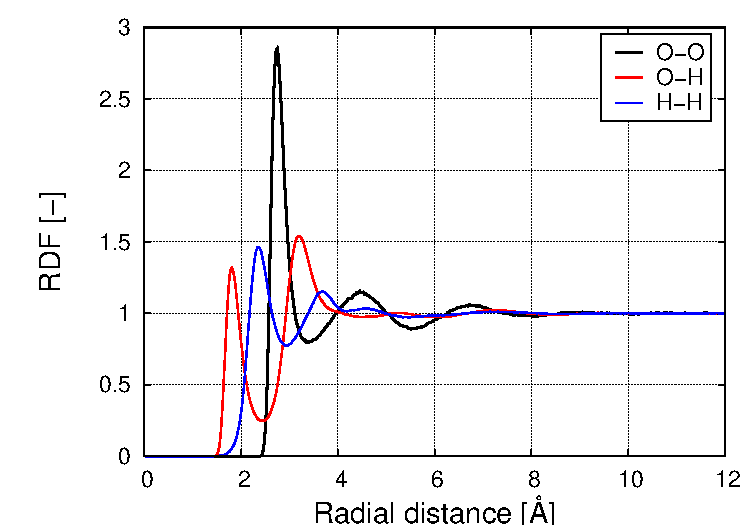
\includegraphics[width=7.5cm]{./Examples/RDFWater.pdf}
  \caption{The radial distribution function of water at 298K.}
  \label{Fig: RDF water}
\end{figure}


\subsection*{Example 13: Measuring bond/bend/dihedral angle distributions MC}

Using Monte Carlo, we can compute the bond/bend/dihedral angle distributions.
The input is given as
\begin{tiny}
\begin{verbatim}
     SimulationType                   MonteCarlo
     NumberOfCycles                   5000000
     NumberOfInitializationCycles     10000
     PrintEvery                       50000
     RestartFile                      no
     
     Forcefield                       ExampleMoleculeForceField
     
     Box 0
     BoxLengths 25 25 25
     ExternalTemperature 298.0
     ExternalPressure 0.0
     ComputeMoleculeProperties yes
     
     component 0 MoleculeName                     2-methylbutane
                 FugacityCoefficient              1.0
                 MoleculeDefinition               ExampleDefinitions
                 TranslationProbability           1.0
                 RotationProbability              1.0
                 ReinsertionProbability           1.0
                 PartialReinsertionProbability    1.0
                 CreateNumberOfMolecules          32
\end{verbatim}
\end{tiny}
The united-atom alkane model describes the CH4, CH3, CH2, CH, and C groups are single, chargeless interaction centers.
The \verb+pseudo_atoms.def+ is defined as
\begin{tiny}
\begin{verbatim}
     #number of pseudo atoms
     5
     #type      print   as    chem  oxidation   mass        charge   polarization B-factor radii  connectivity anisotropic anisotropic-type   tinker-type
     CH4        yes     C     C     0           16.04246    0.0      0.0          1.0      1.00   0            0           relative           0
     CH3        yes     C     C     0           15.03452    0.0      0.0          1.0      1.00   0            0           relative           0
     CH2        yes     C     C     0           14.02658    0.0      0.0          1.0      1.00   0            0           relative           0
     CH         yes     C     C     0           13.01864    0.0      0.0          1.0      1.00   0            0           relative           0
     C          yes     C     C     0           12.0        0.0      0.0          1.0      1.00   0            0           relative           0
\end{verbatim}
\end{tiny}

\noindent
The molecule definition file for a flexible molecule lists all the internal interactions terms, like bond, bend, torsion,
and intra-VDW and charge-charge potentials.
\begin{tiny}
\begin{verbatim}
     # critical constants: Temperature [T], Pressure [Pa], and Acentric factor [-]
     460.35
     3395700.0
     0.2296
     # Number Of Atoms
     5
     # Number Of Groups
     1
     # Alkane-group
     flexible
     # number of atoms
     5
     # atomic positions
     0 CH3
     1 CH
     2 CH2
     3 CH3
     4 CH3
     # Chiral centers Bond  BondDipoles Bend  UrayBradley InvBend  Torsion Imp. Torsion Bond/Bond Stretch/Bend Bend/Bend Stretch/Torsion Bend/Torsion IntraVDW IntraCoulomb
                    0    4            0    4            0       0        2            0         0            0         0               0            0        0            0
     # Bond stretch: atom n1-n2, type, parameters
     0 1 HARMONIC_BOND 96500 1.54
     1 2 HARMONIC_BOND 96500 1.54
     1 4 HARMONIC_BOND 96500 1.54
     2 3 HARMONIC_BOND 96500 1.54
     # Bond bending: atom n1-n2-n3, type, parameters
     0 1 2 HARMONIC_BEND 62500 112
     0 1 4 HARMONIC_BEND 62500 112
     4 1 2 HARMONIC_BEND 62500 112
     1 2 3 HARMONIC_BEND 62500 114
     # Torsion n1-n2-n3-n4 type
     0 1 2 3 TRAPPE_DIHEDRAL   -251.06  428.73  -111.85  441.27
     4 1 2 3 TRAPPE_DIHEDRAL   -251.06  428.73  -111.85  441.27
     # Number of config moves
     4
     # nr fixed, list
     2 0 1
     2 3 2
     3 3 2 1
     4 0 1 2 4
\end{verbatim}
\end{tiny}
To properly sample the internal structure we use the \verb+Reinsertion+-move.
However, the acceptance of this move is often low, especially at high densities and/or low temperatures.
A move that helps is the \verb+PartialReinsertion+ move. This move keeps certain atoms of the molecule fixes, and 
regenerates the others. The \verb+PartialReinsertion+ move is defined by adding 'config'-moves to the molecule definition.
Here, 4 config moves are defined. The first number is the number of fixed atoms, and then a list of the atom identifiers that are kept fixed
(the other atoms are regrown). Note that in CBMC, all branches must be grown simultaneously. That means, you \emph{cannot} keep more than one branch fixes.
The long-range Van der Waals interaction parameters are defined in the \verb+force_field_mixing_rules.def+ file.
\begin{tiny}
\begin{verbatim}
     # general rule for shifted vs truncated
     shifted
     # general rule tailcorrections
     no
     # number of defined interactions
     5
     # type interaction, parameters.
     CH4            lennard-jones    158.5     3.72         // M. G. Martin et al., J. Chem. Phys. 2001, 114, 7174-7181.
     CH3            lennard-jones    108.0     3.76         // D. Dubbeldam et al., J. Phys. Chem. B, 108(33), 12301-12313
     CH2            lennard-jones    56.0      3.96         // idem
     CH             lennard-jones    17.0      4.67         // idem
     C              lennard-jones     0.8      6.38         // idem
     # general mixing rule for Lennard-Jones
     Lorentz-Berthelot
\end{verbatim}
\end{tiny}
The most common (and convenient) way of creating a force field, is to list all defined self-interactions here, and then use a mixture rule to compute
all cross-interactions. The more atom-types you have, the more convenient this becomes.

The acceptance ratios of the partial-reinsertion-move is much high then the reinsertion-move.
This is due to the fact that space already exists at the position of the molecule to regrow parts of its internal structure.
\begin{tiny}
\begin{verbatim}
     Performance of the Reinsertion move:
     ====================================
     Component [2-methylbutane] total tried: 8001488.000000 succesfull growth: 7990960.000000 (99.868424 [%]) accepted: 1114281.000000 (13.925922 [%])
     
     Performance of the partial reinsertion move:
     ============================================
     Component [2-methylbutane] total tried: 7995526.000000 succesfull growth: 7994430.000000 (99.986292 [%]) accepted: 4356062.000000 (54.481244 [%])
\end{verbatim}
\end{tiny}

\subsection*{Example 14: Measuring bond/bend/dihedral angle distributions MD}

We can also compute the angle distributions using MD with the following input:
\begin{tiny}
\begin{verbatim}
     SimulationType                   MolecularDynamics
     NumberOfCycles                   5000000
     NumberOfInitializationCycles     5000
     NumberOfEquilibrationCycles      10000
     PrintEvery                       10000
     
     Ensemble NVT
     
     Forcefield                       ExampleMoleculeForceField
     
     Box 0
     BoxLengths 25 25 25
     ExternalTemperature 298.0
     ExternalPressure 0.0
     ComputeMoleculeProperties yes
     
     component 0 MoleculeName                     2-methylbutane
                 MoleculeDefinition               ExampleDefinitions
                 TranslationProbability           1.0
                 RotationProbability              1.0
                 ReinsertionProbability           1.0
                 CreateNumberOfMolecules          32
\end{verbatim}
\end{tiny}
The distributions can be compared to the Monte Carlo data, ensuring that the grow-algorithm (CBMC) works properly.

\section{Non-basic examples}
\subsection*{Example 1: Adsorption of a binary CO$_2$/CH$_4$ (1:3) mixture in IRMOF-1}

Appreciable adsorption in MOF materials occurs at higher pressure than zeolites, usually in the range up to 10 bar. At these high pressures
absolute and excess adsorption are different, and excess adsorption eventually even goes down. This is due to the fact that excess adsorption is relative
to what would have been in the free pore volume at these conditions. So one can compress the outside fluid but eventually the pores are filled up. At that
maximum absolute loading the excess adsorption will go down.
\begin{tiny}
\begin{verbatim}
     SimulationType                MonteCarlo
     NumberOfCycles                50000
     NumberOfInitializationCycles  5000
     PrintEvery                    1000
     
     Forcefield                    Dubbeldam2007FlexibleIRMOF-1
     
     Framework 0
     FrameworkName IRMOF-1
     UnitCells 1 1 1
     HeliumVoidFraction 0.81
     ExternalTemperature 300.0
     ExternalPressure  10e5
     
     Component 0 MoleculeName               CO2
                 MoleculeDefinition         ExampleDefinitions
                 MolFraction                0.25
                 TranslationProbability     0.5
                 RegrowProbability          0.5
                 IdentityChangeProbability  1.0
                   NumberOfIdentityChanges  2
                   IdentityChangesList      0 1
                 SwapProbability            1.0
                 CreateNumberOfMolecules    0
     
     Component 1 MoleculeName               methane
                 MoleculeDefinition         ExampleDefinitions
                 MolFraction                0.75
                 TranslationProbability     0.5
                 RegrowProbability          0.5
                 IdentityChangeProbability  1.0
                   NumberOfIdentityChanges  2
                   IdentityChangesList      0 1
                 SwapProbability            1.0
                 CreateNumberOfMolecules    0
\end{verbatim}
\end{tiny}

To compute the excess adsorption the void fraction of a structure needs to be specified using `HeliumVoidFraction [real]'. RASPA automatically uses an
equation of state (default: Peng-Robinson) to compute the fugacities from the pressure and mol-fraction as is done here for a mixture of CO$_2$ and CH$_4$.
It also computes the amount of excess molecules from this equation of state.
\begin{tiny}
\begin{verbatim}
     Component 0 [CO2] (Adsorbate molecule)
     
         MoleculeDefinitions: ExampleDefinitions
         Component contains (at least some) atoms which are charged
         Component contains no atoms with point dipoles (polarization)
         Component has a net charge of 0.000000
     
         Ideal chain Rosenbluth weight: 1
         Ideal chain total energy: 0.000000
     
         Critical temparure [K]: 304.128200
         Critical pressure [Pa]: 7377300.000000
         Acentric factor [-]: 0.223940
     
         RXMC partition factor ln(q/V) [ln(A^(-3))]:       0.0000000000
     
         Fluid is a vapour
     
         MolFraction:           0.2500000000 [-]
         Compressibility:       0.9714389725 [-]
     
         Density of the bulk fluid phase:      18.1580726483 [kg/m^3]
     
         Binary mixture EOS parameters:  (0): 0.000000 (1): 0.000000
     
         Amount of excess molecules:       0.8675190741 [-]
     
         Conversion factor molecules/unit cell -> mol/kg:       0.1623747175 [-]
         Conversion factor molecules/unit cell -> mg/g:       7.1442927209 [-]
         Conversion factor molecules/unit cell -> cm^3 STP/gr:       3.6394629804 [-]
         Conversion factor molecules/unit cell -> cm^3 STP/cm^3:       2.1592046669 [-]
         Conversion factor mol/kg -> cm^3 STP/gr:      22.4139757476 [-]
         Conversion factor mol/kg -> cm^3 STP/cm^3:      13.2976654244 [-]
     
         Partial pressure:    250000.00000000000000 [Pa]
                                1874.99999999999977 [Torr]
                                   2.50000000000000 [bar]
                                   2.46730816679003 [atm]
     
         Fugacity coefficient:       0.9503504709 [-]
     
         Partial fugacity:    237587.61773457151139 [Pa]
                                1781.90713300928633 [Torr]
                                   2.37587617734572 [bar]
                                   2.34480747825879 [atm]
     
     Component 1 [methane] (Adsorbate molecule)
     
         MoleculeDefinitions: ExampleDefinitions
         Component contains no atoms with charge
         Component contains no atoms with point dipoles (polarization)
         Component has a net charge of 0.000000
     
         Ideal chain Rosenbluth weight: 1
         Ideal chain total energy: 0.000000
     
         Critical temparure [K]: 190.564000
         Critical pressure [Pa]: 4599200.000000
         Acentric factor [-]: 0.011420
     
         RXMC partition factor ln(q/V) [ln(A^(-3))]:       0.0000000000
     
         Fluid is a vapour
     
         MolFraction:           0.7500000000 [-]
         Compressibility:       0.9714389725 [-]
     
         Density of the bulk fluid phase:       6.6206386115 [kg/m^3]
     
         Binary mixture EOS parameters:  (0): 0.000000 (1): 0.000000
     
         Amount of excess molecules:       2.6025572224 [-]
     
         Conversion factor molecules/unit cell -> mol/kg:       0.1623747175 [-]
         Conversion factor molecules/unit cell -> mg/g:       2.6048899107 [-]
         Conversion factor molecules/unit cell -> cm^3 STP/gr:       3.6394629804 [-]
         Conversion factor molecules/unit cell -> cm^3 STP/cm^3:       2.1592046669 [-]
         Conversion factor mol/kg -> cm^3 STP/gr:      22.4139757476 [-]
         Conversion factor mol/kg -> cm^3 STP/cm^3:      13.2976654244 [-]
     
         Partial pressure:    750000.00000000011642 [Pa]
                                5625.00000000000091 [Torr]
                                   7.50000000000000 [bar]
                                   7.40192450037010 [atm]
     
         Fugacity coefficient:       0.9790119494 [-]
     
         Partial fugacity:    734258.96201743301935 [Pa]
                                5506.94221513074717 [Torr]
                                   7.34258962017433 [bar]
                                   7.24657253409754 [atm]
\end{verbatim}
\end{tiny}
At each `PrintEvery' steps the loadings are shown in a variety of units for both excess and absolute adsorption:
\begin{tiny}
\begin{verbatim}
     Loadings per component:
     ----------------------------------------------------------------------------------------------------------------------------------------------------
     Component 0 (CO2), current number of integer/fractional/reaction molecules: 16/0/0 (avg.  14.98769), density:  67.81662 (avg.  63.52592) [kg/m^3]
         absolute adsorption:  16.00000 (avg.  14.98769) [mol/uc],   2.5979954802 (avg.   2.4336226003) [mol/kg], 114.3086835349 (avg. 107.0764740672) [mg/g]
                               58.2314076859 (avg.  54.5471579425) [cm^3 STP/g],   34.5472746700 (avg.  32.3614991084) [cm^3 STP/cm^3]
         excess adsorption:    15.1324809259 (avg.  14.1201750545) [mol/uc],   2.4571323156 (avg.   2.2927594357) [mol/kg], 108.1108733282 (avg. 100.8786638605) [mg/g]
                               55.0741041308 (avg.  51.3898543873) [cm^3 STP/g],   32.6741234365 (avg.  30.4883478749) [cm^3 STP/cm^3]
     Component 1 (methane), current number of integer/fractional/reaction molecules: 19/0/0 (avg.  19.62858), density:  29.36296 (avg.  30.33438) [kg/m^3]
         absolute adsorption:  19.00000 (avg.  19.62858) [mol/uc],   3.0851196328 (avg.   3.1871849717) [mol/kg],  49.4929083037 (avg.  51.1302874213) [mg/g]
                               69.1497966270 (avg.  71.4374866590) [cm^3 STP/g],   41.0248886706 (avg.  42.3821193995) [cm^3 STP/cm^3]
         excess adsorption:    16.3974427776 (avg.  17.0260217862) [mol/uc],   2.6625301390 (avg.   2.7645954779) [mol/kg],  42.7135332529 (avg.  44.3509123705) [mg/g]
                               59.6778859617 (avg.  61.9655759937) [cm^3 STP/g],   35.4054349701 (avg.  36.7626656990) [cm^3 STP/cm^3]
     ----------------------------------------------------------------------------------------------------------------------------------------------------
\end{verbatim}
\end{tiny}
and at the end error bars are computed for all properties:
\begin{tiny}
\begin{verbatim}
     Component 0 [CO2]
     -------------------------------------------------------------
         Block[ 0] 14.98680           [-]
         Block[ 1] 14.91280           [-]
         Block[ 2] 15.16230           [-]
         Block[ 3] 14.95220           [-]
         Block[ 4] 14.89510           [-]
         ------------------------------------------------------------------------------
         Average loading absolute                             14.9818400000 +/-       0.1327835001 [-]
         Average loading absolute [molecules/unit cell]       14.9818400000 +/-       0.1327835001 [-]
         Average loading absolute [mol/kg framework]                  2.4326720378 +/-       0.0215606833 [-]
         Average loading absolute [milligram/gram framework]        107.0346504582 +/-       0.9486441930 [-]
         Average loading absolute [cm^3 (STP)/gr framework]          54.5258520578 +/-       0.4832606329 [-]
         Average loading absolute [cm^3 (STP)/cm^3 framework]        32.3488588464 +/-       0.2867067530 [-]
     
         Block[ 0] 14.11928           [-]
         Block[ 1] 14.04528           [-]
         Block[ 2] 14.29478           [-]
         Block[ 3] 14.08468           [-]
         Block[ 4] 14.02758           [-]
         ------------------------------------------------------------------------------
         Average loading excess                             14.1143209259 +/-       0.1327835001 [-]
         Average loading excess [molecules/unit cell]       14.1143209259 +/-       0.1327835001 [-]
         Average loading excess [mol/kg framework]                    2.2918088732 +/-       0.0215606833 [-]
         Average loading excess [milligram/gram framework]          100.8368402515 +/-       0.9486441930 [-]
         Average loading excess [cm^3 (STP)/gr framework]            51.3685485027 +/-       0.4832606329 [-]
         Average loading excess [cm^3 (STP)/cm^3 framework]          30.4757076129 +/-       0.2867067530 [-]
     
     Component 1 [methane]
     -------------------------------------------------------------
         Block[ 0] 19.54180           [-]
         Block[ 1] 19.78000           [-]
         Block[ 2] 19.77410           [-]
         Block[ 3] 19.46900           [-]
         Block[ 4] 19.55980           [-]
         ------------------------------------------------------------------------------
         Average loading absolute                             19.6249400000 +/-       0.1774959204 [-]
         Average loading absolute [molecules/unit cell]       19.6249400000 +/-       0.1774959204 [-]
         Average loading absolute [mol/kg framework]                  3.1865940887 +/-       0.0288208499 [-]
         Average loading absolute [milligram/gram framework]         51.1208082045 +/-       0.4623573324 [-]
         Average loading absolute [cm^3 (STP)/gr framework]          71.4242426220 +/-       0.6459898316 [-]
         Average loading absolute [cm^3 (STP)/cm^3 framework]        42.3742620351 +/-       0.3832500198 [-]
     
         Block[ 0] 16.93924           [-]
         Block[ 1] 17.17744           [-]
         Block[ 2] 17.17154           [-]
         Block[ 3] 16.86644           [-]
         Block[ 4] 16.95724           [-]
         ------------------------------------------------------------------------------
         Average loading excess                             17.0223827776 +/-       0.1774959204 [-]
         Average loading excess [molecules/unit cell]       17.0223827776 +/-       0.1774959204 [-]
         Average loading excess [mol/kg framework]                    2.7640045949 +/-       0.0288208499 [-]
         Average loading excess [milligram/gram framework]           44.3414331537 +/-       0.4623573324 [-]
         Average loading excess [cm^3 (STP)/gr framework]            61.9523319566 +/-       0.6459898316 [-]
         Average loading excess [cm^3 (STP)/cm^3 framework]          36.7548083346 +/-       0.3832500198 [-]
\end{verbatim}
\end{tiny}

Also noteworthy is the use of the identity-change move for mixtures. A molecule of a certain type can be changed at the same position into a molecule of
another type. It is specified per component as a list of other components that are allowed for this move. The identity-change move is highly recommended
at high loadings.
\begin{tiny}
\begin{verbatim}
     Performance of the identity change move:
     ======================================
     Component [CO2]->[CO2] total tried: 289262.000000 succesfull growth: 289249.000000 (99.995506 [%]) accepted: 165408.000000 (57.182762 [%])
     Component [CO2]->[methane] total tried: 288518.000000 succesfull growth: 288518.000000 (100.000000 [%]) accepted: 140423.000000 (48.670447 [%])
     Component [methane]->[CO2] total tried: 288616.000000 succesfull growth: 288616.000000 (100.000000 [%]) accepted: 140676.000000 (48.741581 [%])
     Component [methane]->[methane] total tried: 288680.000000 succesfull growth: 288680.000000 (100.000000 [%]) accepted: 274211.000000 (94.987876 [%])
\end{verbatim}
\end{tiny}

\subsection*{Example 2: NPT Monte Carlo of propane}

The density of propane at 250K and 10 bar is about 559.53 kg/m$^3$ (NIST database). In this example the density is
computed using Monte Carlo in the NPT-ensemble. Given the pressure $P$, the temperature $T$, and the amount of molecules $N$,
the density is computed.

\begin{tiny}
\begin{verbatim}
     SimulationType                MonteCarlo
     NumberOfCycles                50000
     NumberOfInitializationCycles  10000
     PrintEvery                    1000
     RestartFile                   no
     
     Forcefield                    ExampleMoleculeForceField
     
     Box 0
     BoxLengths 30 30 30
     ExternalTemperature 250.0
     ExternalPressure 1e6
     ComputeMolecularPressure yes
     
     VolumeChangeProbability       0.05
     
     Component 0 MoleculeName             propane
                 MoleculeDefinition       ExampleDefinitions
                 TranslationProbability   0.5
                 RotationProbability      0.5
                 ReinsertionProbability   0.5
                 CreateNumberOfMolecules  256
\end{verbatim}
\end{tiny}
The simulation for propane gives $568.77\pm 1.99$ kg/m$^3$.
The measured pressure for this short simulation is $10.08\pm1.98$ bar.


\subsection*{Example 3: NPT molecular dynamics of water}
A molecular dynamics simulation of water in the NPT-ensemble
(constant amount of particles $N$, constant average pressure $P$, and constant average temperature $T$).
Many water models are defined, but most are defined with simple Coulombic potentials using cutoffs of 9\AA.
None are optimized with the Ewald-summation except for the re-calibrated Tip5p-Ew model.
Unfortunately, that model is defined using a cutoff always equal to half the box size, while
RASPA uses a fixed cutoff (default: 12 Angstrom). A fixed cutoff is more realistic, but requires the shortest
perpendicular width to be twice the cutoff, thus here larger than 24 \AA. All this results in having
to simulate more than 512 water molecules. The tip5p models use 5 fixed charges placed in the water geometry,
so for each step 2560 charge sites needs to be computed with Ewald. Conclusion: liquid water is computationally
expensive to compute when done properly.

In MD-NPT the average pressure 
$\left\langle P\right\rangle$ and average temperature $\left\langle T\right\rangle$ are imposed. The instantaneous
values, especially for the pressure, are different. RASPA uses the Nose-Hoover chain method, and NPT-MD methods of
Martyna and Tuckermann.

Several options are introduced here: "TimeStep [real]" to set the time step. For rigid molecules the time step can be a bit larger
because the high frequency movement is removed (the O-H is around 3000 cm$^{-1}$). The cutoff can be set with `CutOff [real]'.
The method to compute charge interactions is set with `ChargeMethod [Ewald$|$None]', although Ewald is the default. The precision can specified
using `EwaldPrecision [real]' from which the Ewald parameters $\kappa$ and the amount of wave vectors is inferred.
The initial positions of the water are read from file (`RestartFile yes'), the file is located in directory `RestartInitial/System[int]'.

The experimental density of water at 300K and 1 bar is about 996.56 kg/m$^3$ (NIST database).

\begin{tiny}
\begin{verbatim}
     SimulationType                MolecularDynamics
     NumberOfCycles                100000
     NumberOfInitializationCycles  0
     NumberOfEquilibrationCycles   10000
     PrintEvery                    5000
     RestartFile                   yes
     
     Ensemble                      NPT
     TimeStep                      0.001
     
     ChargeMethod                  Ewald
     CutOff                        10.0
     Forcefield                    Local
     EwaldPrecision                1e-6
     
     Box 0
     BoxLengths 24.83 24.83 24.83
     ExternalTemperature 300.0
     ExternalPressure 1.0e5
     ComputeMSD yes
     PrintMSDEvery 5000
     
     Component 0 MoleculeName             Tip5p
                 MoleculeDefinition       Local
                 TranslationProbability   1.0
                 RotationProbability      1.0
                 ReinsertionProbability   1.0
                 CreateNumberOfMolecules  0
\end{verbatim}
\end{tiny}

The output shows some details of intermediate status during the run: the time run, the current box and average box, etc.
The total linear momentum is conserved and zero (the center of mass movement of the system is removed at initialization).
For this relatively short run, the average pressure of 1.19 $\pm$ 0.62 bar is already quite close to the applied 1 bar,
and the density is 993.4 $\pm$ 2.3 kg/m$^3$.
Also, the temperature of the water, and of the simulation cell (it is a degree of freedom and has therefore an associated temperature)
can also been seen to converge to the applied value of 300K. Energy conservation is adequate with a 0.001 ps time step.

\subsection*{Example 4: Adsorption of CO$_2$ in Na-LTA}

The Linde Type A structure LTA-4A has 96 aluminum per unit cell. A common 4A sample has 96 charge balancing sodium ions.
The ions are small enough to access the sodalite cages, but the bigger methane molecules are exclusively in the big $\alpha$-cages
and not in the sodalite cages. They need to be artificially blocked. 
Because the adsorption is dependent on the positions of the ions it is
important to start from the crystallographic positions and use \emph{only} translation for the ions. Reinsertion moves may transport the ions
to positions in the windows and this is especially important for diffusion (the next example).

\begin{tiny}
\begin{verbatim}
     SimulationType                   MonteCarlo
     NumberOfCycles                   25000
     NumberOfInitializationCycles     10000
     PrintEvery                       1000
     
     Forcefield                       Local
     
     Framework 0
     FrameworkName LTA4A
     RemoveAtomNumberCodeFromLabel yes
     ModifyOxgensConnectedToAluminium yes
     UnitCells 1 1 1
     ExternalTemperature 298.0
     ExternalPressure 10000.0
     
     Component 0 MoleculeName                   sodium
                 MoleculeDefinition             Local
                 TranslationProbability         1.0
                 RandomTranslationProbability   1.0
                 ExtraFrameworkMolecule         yes
                 CreateNumberOfMolecules        96
     
     Component 1 MoleculeName                   CO2
                 MoleculeDefinition             Local
                 BlockPockets                   yes
                 BlockPocketsFilename           LTA
                 TranslationProbability         1.0
                 ReinsertionProbability         1.0
                 SwapProbability                1.0
                 ExtraFrameworkMolecule         no
                 CreateNumberOfMolecules        0
\end{verbatim}
\end{tiny}

\noindent
The force field is taken from Garcia-Sanchez et al.\cite{GarciaSanchez2009}.
Nonframework sodium cations can move freely, adjusting their position depending on their interactions with the framework atoms, 
other sodium cations, and the carbon dioxide molecules.
\begin{tiny}
\begin{verbatim}
     #number of pseudo atoms
     7
     #type      print   as    chem  oxidation   mass        charge   polarization B-factor radii  connectivity anisotropic anisotropic-type   tinker-type
     O          yes     O     O     0           15.9994    -0.39299  0.0          1.0      0.5    2            0           absolute           0
     Oa         yes     Oa     O    0           15.9994    -0.41384  0.0          1.0      0.5    2            0           absolute           0
     Si         yes     Si    Si    0           28.0855     0.78598  0.0          1.0      1.18   4            0           absolute           0
     Al         yes     Al    Al    0           26.981539   0.48598  0.0          1.0      1.18   4            0           absolute           0
     C_co2      yes     C     C     0           12.0        0.6512   0.0          1.0      0.720  0            0           relative           0
     O_co2      yes     O     O     0           15.9994    -0.3256   0.0          1.0      0.68   0            0           relative           0
     Na         yes     Na    Na    0           22.98977    0.3834   0.0          1.0      1.00   0            0           absolute           0
\end{verbatim}
\end{tiny}
The force field uses a different charge for the framework oxygen that is connected to an aluminum atom.
The line
\begin{tiny}
\begin{verbatim}
     ModifyOxgensConnectedToAluminium yes
\end{verbatim}
\end{tiny}
modifies the framework oxygen type 'O' to 'Oa' when the oxygen is found to be connected to an aluminum atom.
For the LTA4A and LTA5A frameworks, \emph{every} oxygen atom is of type 'Oa'.

\noindent 
The file \verb+force_field_mixing_rules.def+ is used to define the CO$_2$ model based on mixing rules
\begin{tiny}
\begin{verbatim}
     # general rule for shifted vs truncated
     shifted
     # general rule tailcorrections
     no
     # number of defined interactions
     4
     # type interaction, parameters.
     O_co2          lennard-jones    85.671    3.017        // A. Garcia-Sanchez et al., J. Phys. Chem. C 2009, 113, 8814-8820.
     C_co2          lennard-jones    29.933    2.745        // idem
     Al             none
     Si             none
     # general mixing rule for Lennard-Jones
     Lorentz-Berthelot
\end{verbatim}
\end{tiny}
The interactions of the CO$_2$ with the zeolite and cations are directly described as pairs.
For that, we can use the \verb+force_field.def+-file.
\begin{tiny}
\begin{verbatim}
     # rules to overwrite
     0
     # number of defined interactions
     13
     # type      type2       interaction
     Na          O           lennard-jones     23.0           3.4        // S. Calero et al., J. Phys. Chem. B 2003, 107(44), 12088-12096.
     Na          Oa          lennard-jones     23.0           3.4        // S. Calero et al., J. Phys. Chem. B 2003, 107(44), 12088-12096.
     Na          C_co2       lennard-jones    362.292         3.320      // A. Garcia-Sanchez et al., J. Phys. Chem. C 2009, 113(20), 8814-8820.
     Na          O_co2       lennard-jones    200.831         2.758      // idem
     O           C_co2       lennard-jones     37.595         3.511      // idem
     O           O_co2       lennard-jones     78.980         3.237      // idem
     Oa          C_co2       lennard-jones     37.595         3.511      // idem
     Oa          O_co2       lennard-jones     78.980         3.237      // idem
     Na          Si          none
     Na          Al          none
     Na          Na          none
     O            O          none
     Oa          Oa          none
     # mixing rules to overwrite
     0
\end{verbatim}
\end{tiny}
The file overwrites any pairs already determined by the mixing rules. Both types of force fields (via mixing rules, and via pairs of interactions)
are commonly found in the literature.

\noindent
Note the line
\begin{tiny}
\begin{verbatim}
     ExtraFrameworkMolecule         yes
\end{verbatim}
\end{tiny}
for the sodium component. This will allow for the computation of the (average) energies between the framework, adsorbates, and cations.
\begin{tiny}
\begin{verbatim}
     Current total potential energy:         -13661140.1319969334 [K]  (avg.   -13660492.8183784448)
         Current Host-Host energy:                     0.0000000000 [K]  (avg.           0.0000000000)
         Current Host-Adsorbate energy:           -38467.0736525305 [K]  (avg.      -39177.6800752787)
         Current Host-Cation energy:           -25997044.5562428236 [K]  (avg.   -25999347.1558655351)
         Current Adsorbate-Adsorbate energy:      -12290.0845394197 [K]  (avg.      -11985.7555443291)
         Current Cation-Cation energy:          12511975.9583617374 [K]  (avg.    12512947.5563156120)
         Current Adsorbate-Cation energy:        -125314.3759244105 [K]  (avg.     -122929.7832096771)
\end{verbatim}
\end{tiny}
Also note the line
\begin{tiny}
\begin{verbatim}
     RandomTranslationProbability   1.0
\end{verbatim}
\end{tiny}
Because of the large energies involved when using cations, the CBMC biasing algorithms might experience numerical under/overflow.
Since the sodium-ion is a small molecule, the reinsertion (which is biased) can be replaced with a random translation.
For a single atom molecules, both do the same thing: a reinsertion randomly in the simulation box.

\noindent
Lastly, LTA contains pockets called $\beta$-cages that are not accessible from the main large cavities called $\alpha$-cages.
In MC, the reinsertion and swap-move pick random location inside the simulation cell volume, and therefore we need to artificially block
the inaccessible pockets. For that, we can a blocking file, here names \verb+LTA.block+.
\begin{tiny}
\begin{verbatim}
     BlockPockets yes 
     BlockPocketsFilename LTA
\end{verbatim}
This file basically contains 32 pockets with a fractional center point and a radius in Angstrom.
\end{tiny}
\begin{tiny}
\begin{verbatim}
     32
     0.0        0.0         0.0        4.0
     0.5        0.0         0.0        4.0
     0.0        0.5         0.0        4.0
     0.5        0.5         0.0        4.0
     ...
\end{verbatim}
\end{tiny}
Any MC move that picks a random CO$_2$ location inside this volume will be automatically rejected.

\subsection*{Example 5: Diffusion of CO$_2$ in Na-LTA}

An example of molecular dynamics of an adsorbate (CO$_2$) diffusing through the pores of LTA 4A loaded with ions.
The mean-square displacement is computed during the run.

\begin{tiny}
\begin{verbatim}
     SimulationType                   MolecularDynamics
     NumberOfCycles                   250000
     NumberOfInitializationCycles     5000
     NumberOfEquilibrationCycles      10000
     PrintEvery                       5000
     RestartFile                      no
     
     Ensemble                         NVT
     
     Forcefield                       Local
     ModifyOxgensConnectedToAluminium yes
     TimeStep                         0.0005
     
     Framework 0
     FrameworkName LTA4A
     RemoveAtomNumberCodeFromLabel yes
     UnitCells 1 1 1
     ExternalTemperature 600.0
     ComputeMSD yes
     PrintMSDEvery 5000
     
     component 0 MoleculeName             sodium
                 MoleculeDefinition       Local
                 TranslationProbability   1.0
                 ReinsertionProbability   1.0
                 ExtraFrameworkMolecule   yes
                 CreateNumberOfMolecules  96
     
     component 1 MoleculeName             CO2
                 MoleculeDefinition       Local
                 BlockPockets             yes
                 BlockPocketsFilename     LTA
                 TranslationProbability   1.0
                 RotationProbability      1.0
                 ReinsertionProbability   1.0
                 ExtraFrameworkMolecule   no
                 CreateNumberOfMolecules  64
\end{verbatim}
\end{tiny}

\noindent
The examples shows that diffusion, even of small molecules, can be \emph{very} slow in nanoporous materials.
In 120 ps, the MSD is below 50 \AA$^2$, meaning the adsorbates have not moved further than 7.1 \AA.
In LTA4A, the cations tend to sit in the windows separating the cages.
Therefore, diffusion in these types of systems might not be accessible to MD, and techniques like Transitions State Theory (TST)
have to be used.

\subsection*{Example 6: Diffusion of benzene in rigid IRMOF-1}

Benzene (and aromatic molecules in general) are usually kept rigid. RASPA uses quaternions for the description of the
orientation of the molecules. The integration schemes of Martyna and Tuckermann are symplectic and conserve energy
very well. Even though the molecule is described as a center of mass and a orientation, the forces are still computed
atomically. In this example the diffusivity the mean-square displacement of benzene at 298K in IRMOF-1 is computed.
The forcefield is specifically
optimized for iso-reticular metal-organic frameworks \cite{Dubbeldam2007}.
The force field for benzene is taken from Rai and Siepmann \cite{Rai2007}.

\begin{tiny}
\begin{verbatim}
     SimulationType                MolecularDynamics
     NumberOfCycles                100000
     NumberOfEquilibrationCycles   10000
     NumberOfInitializationCycles  1000
     PrintEvery                    5000
     RestartFile                   no
     
     Ensemble                      NVT
     
     ChargeMethod                  Ewald
     CutOff                        12.0
     TimeStep                      0.0005
     Forcefield                    Local
     EwaldPrecision                1e-6
     
     Framework 0
     FrameworkName IRMOF-1
     UnitCells 1 1 1
     ExternalTemperature 298.0
     
     Component 0 MoleculeName              benzene
                 MoleculeDefinition        Local
                 IdealGasRosenbluthWeight  1.0
                 TranslationProbability    1.0
                 RotationProbability       1.0
                 ReinsertionProbability    1.0
                 CreateNumberOfMolecules   16
\end{verbatim}
\end{tiny}

\begin{tiny}
\begin{verbatim}
     Conserved energy:      -36557.3872141186 Energy drifts:  0.0000001015           0.0000059765
     Temperature:             307.434 (avg.  298.597), Translational (avg.  300.133), Rotational (avg.  297.060)
     Temperature Adsorbates:  307.434 (avg.  298.597), Translational (avg.  300.133), Rotational (avg.  297.060)
\end{verbatim}
\end{tiny}

\begin{figure}[t]
  \centering
  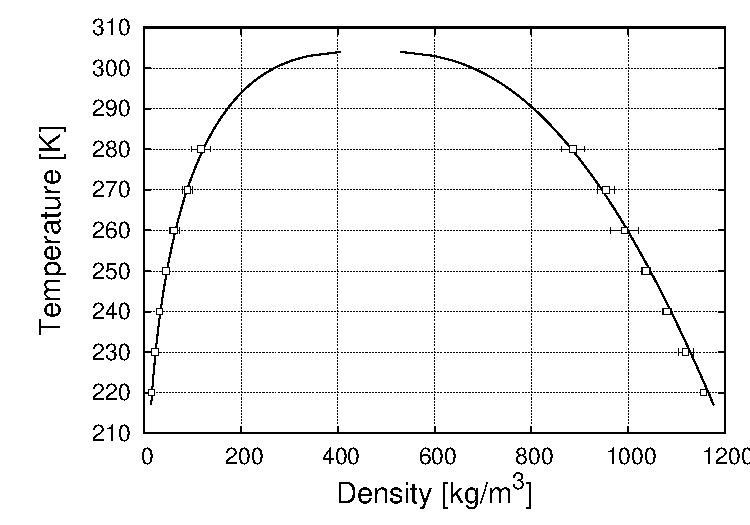
\includegraphics[width=7.5cm]{./Examples/GibbsCO2.pdf}
  \caption{Gibbs ensemble simulation of CO$_2$ at 250K. Two simulation boxes are used: one for the gas-branch and one for the liquid branch. The simulation can
           only be conducted below a certain temperature because otherwise the boxes can swap between gas and liquid. At 250K, the boxes are initialized
           with an equal amount of molecules, but soon split into gas and liquid. The average densities are straightforward to measure. As shown, the
           model for CO$_2$ does a good job when compare to experimental data (NIST database).}
  \label{Fig: Gibbs CO2}
\end{figure}

\subsection*{Example 7: Gibbs ensemble simulation of CO$_2$}

The Gibbs ensemble is way of computing coexistence without interfaces. It is one the most used methods
to study vapor-liquid and liquid-liquid equilibria, it is not suitable for very dense systems. The 
conditions for coexistence of two or more phases I, II, \dots is that the pressure and temperature 
of all the phases must be equal, as well as the chemical potential of all the species. The Gibbs
ensemble example for the single component CO$_2$ is listed below. two boxes will be used, one will
correspond to the liquid phase, the other one to the gas phase. The `GibbsVolumeChange' move
changes the individual volume leaving the total volume in tact, the `GibbsSwap' move
swaps particles from one box to the other. One of the practical problems is to make sure both
boxes remain larger than twice the cutoff length. If not, the program will exit with an error message,
and the simulation should be restarted with a bigger volume. 
Note that RASPA uses orientational biased insertions for small rigid molecules like CO$_2$.
For this example about 10000-20000 cycles are needed to equilibrate properly.
\begin{tiny}
\begin{verbatim}
     SimulationType                MonteCarlo
     NumberOfCycles                25000
     NumberOfInitializationCycles  10000
     PrintEvery                    1000
     RestartFile                   no
     
     Forcefield                    ExampleMoleculeForceField
     
     Box 0
     BoxLengths 30 30 30
     BoxAngles 90 90 90
     ExternalTemperature 240.0
     
     Box 1
     BoxLengths 30 30 30
     BoxAngles 90 90 90
     ExternalTemperature 240.0
     
     GibbsVolumeChangeProbability 0.1
     
     Component 0 MoleculeName             CO2
                 MoleculeDefinition       ExampleDefinitions
                 TranslationProbability   1.0
                 RotationProbability      1.0
                 ReinsertionProbability   1.0
                 GibbsSwapProbability     1.0
                 CreateNumberOfMolecules  150 150
\end{verbatim}
\end{tiny}
The computed densities are
\begin{tiny}
\begin{verbatim}
     Average density component 0 [CO2]
     -------------------------------------------------------------
         Block[ 0]           33.53583 [kg/m^3]
         Block[ 1]           33.36214 [kg/m^3]
         Block[ 2]           34.55914 [kg/m^3]
         Block[ 3]           34.05442 [kg/m^3]
         Block[ 4]           34.14516 [kg/m^3]
         ------------------------------------------------------------------------------
         Average             33.93134 [kg/m^3] +/-            0.60035 [kg/m^3]
     
     Average density component 0 [CO2]
     -------------------------------------------------------------
         Block[ 0]         1104.22167 [kg/m^3]
         Block[ 1]         1103.62933 [kg/m^3]
         Block[ 2]         1101.86174 [kg/m^3]
         Block[ 3]         1107.16121 [kg/m^3]
         Block[ 4]         1106.36198 [kg/m^3]
         ------------------------------------------------------------------------------
         Average           1104.64719 [kg/m^3] +/-            2.65080 [kg/m^3]
\end{verbatim}
\end{tiny}
The experimental densities at 240K are 33.295 and 1088.9 kg/m$^3$ respectively.

\noindent
In the high density phase, the acceptance probabilities of the reinsertion-move and Gibbs swap-move are low.
The Gibbs volume change is adjusted to achieve roughly 50\% acceptance.
\begin{tiny}
\begin{verbatim}
     Performance of the Reinsertion move:
     ====================================
     Component [CO2] total tried: 1730548.000000 succesfull growth: 1421729.000000 (82.154843 [%]) accepted: 18572.000000 (1.073186 [%])
     
     Performance of the Gibbs volume change move:
     ============================================
     total tried: 346089.000000 accepted: 206146.000000 (59.564447 [%])
         maximum volume change 0.049783
     
     Performance of the Gibbs swap move:
     ============================================
     Component [CO2] transfered to system [0] total tried: 1729616.000000 accepted: 83910.000000 (4.851366 [%])
\end{verbatim}
\end{tiny}


\subsection*{Example 8: Minimization of octane}

Energy minimization is often used to understand the behavior of molecules.
This example shows the input for the minimization of octane using a united-atom model\cite{Dubbeldam2004}.
\begin{tiny}
\begin{verbatim}
     SimulationType                Minimization
     NumberOfCycles                10
     NumberOfInitializationCycles  100
     RestartFile                   no
     PrintEvery                    100
     
     MaximumNumberOfMinimizationSteps 1000
     RMSGradientTolerance 1e-6
     MaxGradientTolerance 1e-6
     
     RemoveTranslationFromHessian yes
     RemoveRotationFromHessian yes
     
     Ensemble        NVT
     
     Forcefield      ExampleMoleculeForceField
     ChargeMethod    Coulomb
     CutOffCoulomb   15.0
     
     Box 0
     BoxLengths 30 30 30
     UnitCells 1 1 1
     ExternalTemperature 298.0
     Movies yes
     WriteMoviesEvery 1
     
     Component 0 MoleculeName             octane
                 MoleculeDefinition       ExampleDefinitions
                 TranslationProbability   0.5
                 RotationProbability      0.5
                 ReinsertionProbability   0.5
                 CreateNumberOfMolecules  1
\end{verbatim}
\end{tiny}
Note that the minimization algorithm guarantees that all positive eigenvalues are found.
The first 6 eigenvalues are zero, corresponding to translation and rotation of the isolated octane molecule.
A requirement is that all the forces are zero.
\begin{tiny}
\begin{verbatim}
     Forces
     Adsorbate[0] Atom: 0  3.90833e-10 1.43088e-10 6.56558e-10
     Adsorbate[0] Atom: 1  -9.72811e-10 -2.7887e-10 -7.84603e-10
     Adsorbate[0] Atom: 2  5.27156e-10 6.9297e-11 3.52394e-11
     Adsorbate[0] Atom: 3  -1.91779e-10 -1.80862e-10 -6.57963e-11
     Adsorbate[0] Atom: 4  6.83851e-10 1.25738e-09 5.36808e-10
     Adsorbate[0] Atom: 5  -1.2857e-09 -3.34806e-09 -1.38364e-09
     Adsorbate[0] Atom: 6  1.11448e-09 3.29423e-09 1.90479e-09
     Adsorbate[0] Atom: 7  -2.66031e-10 -9.56199e-10 -8.99352e-10
\end{verbatim}
\end{tiny}
The minimization needs to be repeated many times from different initial conditions.
Here, there 10 minimization attempts with 100 cycles of MC initialization at 298K.
\begin{tiny}
\begin{verbatim}
     Final energy after minimization:     479.7192896697 in 7 steps
     Final energy after minimization:    -207.1377558989 in 6 steps
     Final energy after minimization:     516.7656903515 in 7 steps
     Final energy after minimization:     491.0018422214 in 7 steps
     Final energy after minimization:     471.6063292385 in 8 steps
     Final energy after minimization:    -207.1377558989 in 6 steps
     Final energy after minimization:     523.2720371093 in 7 steps
     Final energy after minimization:     134.0679023161 in 6 steps
     Final energy after minimization:    -207.1377558989 in 6 steps
     Final energy after minimization:     119.7394458177 in 6 steps
\end{verbatim}
\end{tiny}
The results are usually "groups" of energies corresponding to a specific configuration.
The lowest in energy is the stretched-out, linear configuration.

\subsection*{Example 9: Adsorption of hexane-isomers in MFI}

Adsorption selectivities are computed by simulating a multiple-component mixture where the molecules compete for adsorption sites.
In this example, the adsorption of hexane-isomers in MFI at 433 K and 2000 Pa is computed.
Before running this, the ideal Rosenbluth values for the molecules at the desired temperature need to be computed (see Auxiliary examples).
The identity-change move is used to try to change the identity to any type of molecule (including itself).
Also partial-reinsertion moves are defined for all the adsorbates.
We also define \verb+FugacityCoefficient 1.0+ for all components, which means we do a simulation at a \emph{fugacity} (not pressure) of 2000 Pa.
\begin{tiny}
\begin{verbatim}
     SimulationType                MonteCarlo
     NumberOfCycles                200000
     NumberOfInitializationCycles  200000
     PrintEvery                    5000
     RestartFile                   no
     
     ChargeMethod                  None
     Forcefield                    ExampleZeolitesForceField
     CutOffVDW                     12.0
     RemoveAtomNumberCodeFromLabel yes
     
     Framework             0
     FrameworkName         MFI_SI
     UseChargesFromCIFFile no
     UnitCells             2 2 2
     HeliumVoidFraction    0.29
     ExternalTemperature   433.0
     ExternalPressure      2000.0
     
     Component 0 MoleculeName                   hexane
                 MoleculeDefinition             Local
                 IdealGasRosenbluthWeight       0.00811779
                 FugacityCoefficient            1.0
                 TranslationProbability         1.0
                 RotationProbability            1.0
                 ReinsertionProbability         1.0
                 PartialReinsertionProbability  1.0
                 IdentityChangeProbability      1.0
                   NumberOfIdentityChanges      4
                   IdentityChangesList          0 1 2 3
                 SwapProbability                1.0
                 CreateNumberOfMolecules        0
     
     Component 1 MoleculeName                   2-methylpentane
                 MoleculeDefinition             Local
                 IdealGasRosenbluthWeight       0.0470006
                 FugacityCoefficient            1.0
                 TranslationProbability         1.0
                 RotationProbability            1.0
                 ReinsertionProbability         1.0
                 PartialReinsertionProbability  1.0
                 IdentityChangeProbability      1.0
                   NumberOfIdentityChanges      4
                   IdentityChangesList          0 1 2 3
                 SwapProbability                1.0
                 CreateNumberOfMolecules        0
     
     Component 2 MoleculeName                   3-methylpentane
                 MoleculeDefinition             Local
                 IdealGasRosenbluthWeight       0.0536003
                 FugacityCoefficient            1.0
                 TranslationProbability         1.0
                 RotationProbability            1.0
                 ReinsertionProbability         1.0
                 PartialReinsertionProbability  1.0
                 IdentityChangeProbability      1.0
                   NumberOfIdentityChanges      4
                   IdentityChangesList          0 1 2 3
                 SwapProbability                1.0
                 CreateNumberOfMolecules        0
     
     Component 3 MoleculeName                   22-dimethylbutane
                 MoleculeDefinition             Local
                 IdealGasRosenbluthWeight       0.226526
                 FugacityCoefficient            1.0
                 TranslationProbability         1.0
                 RotationProbability            1.0
                 ReinsertionProbability         1.0
                 PartialReinsertionProbability  1.0
                 IdentityChangeProbability      1.0
                   NumberOfIdentityChanges      4
                   IdentityChangesList          0 1 2 3
                 SwapProbability                1.0
                 CreateNumberOfMolecules        0
\end{verbatim}
\end{tiny}

\begin{tiny}
\begin{verbatim}
Component 0 [hexane]
-------------------------------------------------------------
    Average loading absolute [molecules/unit cell]        1.2595631250 +/-       0.0066198404 [-]

Component 1 [2-methylpentane]
    Average loading absolute [molecules/unit cell]        0.6311325000 +/-       0.0086401923 [-]

Component 2 [3-methylpentane]
-------------------------------------------------------------
    Average loading absolute [molecules/unit cell]        0.2982025000 +/-       0.0080754705 [-]

Component 3 [22-dimethylbutane]
-------------------------------------------------------------
    Average loading absolute [molecules/unit cell]        0.1239156250 +/-       0.0013021057 [-]
\end{verbatim}
\end{tiny}

\begin{tiny}
\begin{verbatim}
     Performance of the swap addition move:
     ======================================
     Component [hexane] total tried: 343107.000000 succesfull growth: 225219.000000 (65.641039 [%]) accepted: 20776.000000 (6.055254 [%])
     Component [2-methylpentane] total tried: 341490.000000 succesfull growth: 212073.000000 (62.102258 [%]) accepted: 10655.000000 (3.120150 [%])
     Component [3-methylpentane] total tried: 342604.000000 succesfull growth: 205370.000000 (59.943842 [%]) accepted: 10411.000000 (3.038785 [%])
     Component [22-dimethylbutane] total tried: 341932.000000 succesfull growth: 193866.000000 (56.697238 [%]) accepted: 9767.000000 (2.856416 [%])
     
     Performance of the swap deletion move:
     ======================================
     Component [hexane] total tried: 342845.000000 succesfull growth: 342845.000000 (100.000000 [%]) accepted: 20563.000000 (5.997754 [%])
     Component [2-methylpentane] total tried: 342464.000000 succesfull growth: 341147.000000 (99.615434 [%]) accepted: 10612.000000 (3.098720 [%])
     Component [3-methylpentane] total tried: 342281.000000 succesfull growth: 313715.000000 (91.654226 [%]) accepted: 10675.000000 (3.118783 [%])
     Component [22-dimethylbutane] total tried: 342573.000000 succesfull growth: 218648.000000 (63.825228 [%]) accepted: 9761.000000 (2.849320 [%])
     
     Performance of the Reinsertion move:
     ====================================
     Component [hexane] total tried: 682800.000000 succesfull growth: 459936.000000 (67.360281 [%]) accepted: 9769.000000 (1.430726 [%])
     Component [2-methylpentane] total tried: 679289.000000 succesfull growth: 434051.000000 (63.897840 [%]) accepted: 4340.000000 (0.638903 [%])
     Component [3-methylpentane] total tried: 627118.000000 succesfull growth: 385061.000000 (61.401682 [%]) accepted: 4115.000000 (0.656176 [%])
     Component [22-dimethylbutane] total tried: 436366.000000 succesfull growth: 252934.000000 (57.963728 [%]) accepted: 3080.000000 (0.705830 [%])
\end{verbatim}
\end{tiny}

\begin{tiny}
\begin{verbatim}
     Performance of the partial reinsertion move:
     ============================================
     Component [hexane] total tried: 683886.000000 succesfull growth: 661852.000000 (96.778118 [%]) accepted: 158568.000000 (23.186321 [%])
     Component [2-methylpentane] total tried: 681914.000000 succesfull growth: 679831.000000 (99.694536 [%]) accepted: 256922.000000 (37.676599 [%])
     Component [3-methylpentane] total tried: 627634.000000 succesfull growth: 625746.000000 (99.699188 [%]) accepted: 176488.000000 (28.119573 [%])
     Component [22-dimethylbutane] total tried: 437324.000000 succesfull growth: 435874.000000 (99.668438 [%]) accepted: 210354.000000 (48.100264 [%])
     
     Performance of the identity change move:
     ======================================
     Component [hexane]->[hexane] total tried: 170814.000000 succesfull growth: 153200.000000 (89.688199 [%]) accepted: 11192.000000 (6.552156 [%])
     Component [hexane]->[2-methylpentane] total tried: 171350.000000 succesfull growth: 143781.000000 (83.910709 [%]) accepted: 5675.000000 (3.311935 [%])
     Component [hexane]->[3-methylpentane] total tried: 170612.000000 succesfull growth: 137177.000000 (80.402902 [%]) accepted: 5576.000000 (3.268234 [%])
     Component [hexane]->[22-dimethylbutane] total tried: 171284.000000 succesfull growth: 136622.000000 (79.763434 [%]) accepted: 4771.000000 (2.785432 [%])
     Component [2-methylpentane]->[hexane] total tried: 170176.000000 succesfull growth: 162611.000000 (95.554602 [%]) accepted: 5714.000000 (3.357700 [%])
     Component [2-methylpentane]->[2-methylpentane] total tried: 169789.000000 succesfull growth: 163167.000000 (96.099865 [%]) accepted: 9153.000000 (5.390809 [%])
     Component [2-methylpentane]->[3-methylpentane] total tried: 170132.000000 succesfull growth: 156426.000000 (91.943902 [%]) accepted: 4905.000000 (2.883056 [%])
     Component [2-methylpentane]->[22-dimethylbutane] total tried: 170500.000000 succesfull growth: 164951.000000 (96.745455 [%]) accepted: 8378.000000 (4.913783 [%])
     Component [3-methylpentane]->[hexane] total tried: 156737.000000 succesfull growth: 143803.000000 (91.747960 [%]) accepted: 5459.000000 (3.482904 [%])
     Component [3-methylpentane]->[2-methylpentane] total tried: 156602.000000 succesfull growth: 140396.000000 (89.651473 [%]) accepted: 4772.000000 (3.047215 [%])
     Component [3-methylpentane]->[3-methylpentane] total tried: 156796.000000 succesfull growth: 135085.000000 (86.153346 [%]) accepted: 8233.000000 (5.250772 [%])
     Component [3-methylpentane]->[22-dimethylbutane] total tried: 156055.000000 succesfull growth: 134198.000000 (85.994041 [%]) accepted: 3891.000000 (2.493352 [%])
     Component [22-dimethylbutane]->[hexane] total tried: 109564.000000 succesfull growth: 104319.000000 (95.212844 [%]) accepted: 4638.000000 (4.233142 [%])
     Component [22-dimethylbutane]->[2-methylpentane] total tried: 108833.000000 succesfull growth: 104601.000000 (96.111474 [%]) accepted: 8506.000000 (7.815644 [%])
     Component [22-dimethylbutane]->[3-methylpentane] total tried: 109359.000000 succesfull growth: 100691.000000 (92.073812 [%]) accepted: 3902.000000 (3.568065 [%])
     Component [22-dimethylbutane]->[22-dimethylbutane] total tried: 109054.000000 succesfull growth: 106124.000000 (97.313258 [%]) accepted: 7485.000000 (6.863572 [%])
\end{verbatim}
\end{tiny}

\section{Advanced examples}

\subsection*{Example 1: Adsorption of CO$_2$ in using the Gibbs-ensemble}

The Gibbs ensemble method can be used to compute adsorption isotherms in nanoporous materials \cite{Panagiotopoulos1987,McGrother1999}.
One of the boxes contains the framework, while the other box contains the fluid-phase
(either gas or liquid) that is in equilibrium with the adsorbed phase.
For adsorption of a system of n components, the Gibbs phase rule requires that n+1 intensive variables be set,
if you consider the adsorbent as an additional component.  These n+1 variables are conveniently taken as the
temperature, the pressure of the fluid phase, and n-1 mole fractions in the fluid phase.
The system is then simulated using the NpT Gibbs ensemble.
The fluid-phase box is maintained at constant pressure (and temperature) by applying volume-moves.
For the simulation of adsorption in a rigid framework the volume
moves on the adsorbed-phase box are switched off; there is no requirement for mechanical equilibrium \cite{Panagiotopoulos1987}.
The equilibrium constraints are equal temperature in both systems and equal chemical potentials
in the bulk and in the interior of the framework (similar to the VLE, the chemical potential equilibrium is
enforced by particle swap moves between the boxes).

\begin{tiny}
\begin{verbatim}
     SimulationType                MonteCarlo
     NumberOfCycles                25000
     NumberOfInitializationCycles  5000
     PrintEvery                    1000
     
     Forcefield                    ExampleZeolitesForceField
     RemoveAtomNumberCodeFromLabel yes
     
     Framework 0
     FrameworkName MFI_SI
     UnitCells 2 2 2
     HeliumVoidFraction 0.29
     ExternalTemperature 300.0
     ExternalPressure 1e4
     
     Box 1
     BoxLengths 110 110 110
     CutOffCoulomb 50
     ExternalTemperature 300.0
     ExternalPressure 1e4
     
     VolumeChangeProbability 0.2
     
     Component 0 MoleculeName             methane
                 MoleculeDefinition       ExampleDefinitions
                 TranslationProbability   0.5
                 ReinsertionProbability   0.5
                 GibbsSwapProbability     1.0
                 CreateNumberOfMolecules  0 100
\end{verbatim}
\end{tiny}

The absolute loading is 2.77$\pm$ 0.05 vs 2.76$\pm$ 0.02 in example 6 of the basic-examples.

\subsection*{Example 2: Benzene diffusion in flexible IRMOF-10}

Molecules with a phenyl-ring are usually quite rigid. In Monte Carlo, rigid units are not a problem, because the MC moves can be developed in such a way that the
constraints remain satisfied, i.e. translation and rotation of the whole rigid unit. In molecular dynamics, there are two general approaches. The first is to integrate
the molecules atomically and afterwards satisfy the constraints iteratively using for example the shake algorithm. For bigger molecules complications arise, convergence
becomes more difficult, and for a planar molecule like benzene additional sites above the molecule are needed. Therefore, the second approach has become more popular. 
Using quaternions (or Euler angles) one can describe the configurations of the molecule as a center-of-mass position and an orientation. The translation and rotation
are integrated and when the forces are needed the atoms positions are computed from the com position and the orientation. The forces are then summed to the center of mass
and the torque is computed. Miller et al. have developed an integration algorithm for rigid units (using quaternions) that is symplectic\cite{Miller2002}.

All these techniques are combined in the example of diffusion of benzene in IRMOF-10. The integration is performed in the NVT ensemble using the Nose-Hoover thermostats.
Three separate Nose-Hoover chains are operating on (i) the translation, (ii) the rotation of the molecules, and (iii) on the framework.

\begin{tiny}
\begin{verbatim}
     SimulationType                MolecularDynamics
     NumberOfCycles                1000000
     NumberOfEquilibrationCycles   10000
     NumberOfInitializationCycles  100
     PrintEvery                    5000
     RestartFile                   no
     
     Ensemble                      NVT
     
     ChargeMethod                  Ewald
     CutOff                        12.0
     TimeStep                      0.0005
     Forcefield                    Local
     EwaldPrecision                1e-6
     
     Framework 0
     FrameworkName IRMOF-10
     UnitCells 1 1 1
     ExternalTemperature 298.0
     Movies no
     WriteMoviesEvery 1000
     
     FrameworkDefinitions Local
     FlexibleFramework yes
     
     Component 0 MoleculeName              benzene
                 MoleculeDefinition        ExampleDefinitions
                 IdealGasRosenbluthWeight  1.0
                 TranslationProbability    1.0
                 RotationProbability       1.0
                 ReinsertionProbability    1.0
                 CreateNumberOfMolecules   16
\end{verbatim}
\end{tiny}

\begin{tiny}
\begin{verbatim}
     #number of pseudo atoms
     12
     #type      print   as    chem  oxidation   mass        charge   polarization B-factor radii  connectivity anisotropic anisotropic-type   tinker-type
     Zn1        yes     Zn    Zn    0           65.37       1.275    0.0          1.0      1.448  0            0           relative           0
     O1         yes     O     O     0           15.9994    -1.5      0.0          1.0      0.68   2            0           relative           0
     O2         yes     O     O     0           15.9994    -0.6      0.0          1.0      0.68   2            0           relative           0
     C1         yes     C     C     0           12.0107     0.475    0.0          1.0      0.720  0            0           relative           0
     C2         yes     C     C     0           12.0107     0.125    0.0          1.0      0.720  0            0           relative           0
     C3         yes     C     C     0           12.0107    -0.15     0.0          1.0      0.720  0            0           relative           0
     C4         yes     C     C     0           12.0107    -0.15     0.0          1.0      0.720  0            0           relative           0
     C5         yes     C     C     0           12.0107     0.0      0.0          1.0      0.720  0            0           relative           0
     H1         yes     H     H     0           1.00794     0.15     0.0          1.0      0.320  0            0           relative           0
     H2         yes     H     H     0           1.00794     0.15     0.0          1.0      0.320  0            0           relative           0
     C_benz     yes     C     C     0           12.0       -0.095    0.0          1.0      0.70   0            0           relative           0
     H_benz     yes     H     H     0           1.00794     0.095    0.0          1.0      0.320  0            0           relative           0
\end{verbatim}
\end{tiny}

\noindent
The force field for IRMOF-10 is taken from Dubbeldam et al.\cite{Dubbeldam2007}. It is a re-parameterization and extension of the flexible IRMOF-1
model of Greathouse and Allendorf\cite{Greathouse2008}.
The model for the benzene adsorbate is taken from Rai and Siepmann\cite{Rai2007}.
\begin{tiny}
\begin{verbatim}
     # general rule for shifted vs truncated
     shifted
     # general rule tailcorrections
     no
     # number of defined interactions
     12
     # type interaction
     Zn1            lennard-jones    0.42      2.7        // D. Dubbeldam, K.S. Walton, D.E. Ellis, R.Q. Snurr, Angew. Chem. Int. Ed. 2007, 46, 4496-4499.
     O1             lennard-jones    700.0     2.98       // idem
     O2             lennard-jones    70.5      3.11       // idem
     C1             lennard-jones    47.0      3.74       // idem
     C2             lennard-jones    47.86     3.47       // idem
     C3             lennard-jones    47.86     3.47       // idem
     C4             lennard-jones    47.86     3.47       // idem
     C5             lennard-jones    47.86     3.47       // idem
     H1             lennard-jones    7.65      2.85       // idem
     H2             lennard-jones    7.65      2.85       // idem
     C_benz         lennard-jones    30.70     3.60       // N. Rai and J.I. Siepmann, J. Phys. Chem. B 2007, 111, 10790-10799.
     H_benz         lennard-jones    25.45     2.36       // idem
     # general mixing rule for Lennard-Jones
     Lorentz-Berthelot
\end{verbatim}
\end{tiny}

\noindent
Molecule files are defined in terms of their numerical identifiers (starting from number zero).
This would be cumbersome for framework file to enumerated all bonds, bends, torsions etc.
Therefore, the framework file can be constructed in terms of atom \emph{types}.
\begin{tiny}
\begin{verbatim}
     #CoreShells bond  BondDipoles UreyBradley bend  inv  tors improper-torsion bond/bond bond/bend bend/bend stretch/torsion bend/torsion
               0    8            0           0   12    0    14                5         0         0         0               0            0
     #bond stretch atom n1-n2, equilibrium distance, bondforce-constant
     O2 C1  HARMONIC_BOND  543840.64928424  1.25
     C1 C2  HARMONIC_BOND  353750.919316375 1.42
     C2 C3  HARMONIC_BOND  483413.91047488  1.36
     C3 C4  HARMONIC_BOND  483413.91047488  1.36
     C4 C5  HARMONIC_BOND  483413.91047488  1.36
     C3 H1  HARMONIC_BOND  366001.13136396  0.95
     C4 H2  HARMONIC_BOND  366001.13136396  0.95
     C5 C5  HARMONIC_BOND  483413.91047488  1.36
     #bond bending atom n1-n2-n3, equilibrium angle, bondforce-constant
     O2 C1 O2 HARMONIC_BEND 135960.162321060 130.0
     O2 C1 C2 HARMONIC_BEND 54882.4848123699 115.0
     C1 C2 C3 HARMONIC_BEND 34926.5543205787 120.0
     C2 C3 C4 HARMONIC_BEND 90640.10821404 120.0
     C3 C4 C5 HARMONIC_BEND 90640.10821404 120.0
     C3 C2 C3 HARMONIC_BEND 90640.10821404 120.0
     C4 C5 C4 HARMONIC_BEND 90640.10821404 120.0
     C4 C5 C5 HARMONIC_BEND 90640.10821404 120.0
     C4 C3 H1 HARMONIC_BEND 37263.15559911 120.0
     C2 C3 H1 HARMONIC_BEND 37263.15559911 120.0
     C3 C4 H2 HARMONIC_BEND 37263.15559911 120.0
     C5 C4 H2 HARMONIC_BEND 37263.15559911 120.0
     #torsion atom n1-n2-n3-n4,
     O2 C1 C2 C3  TRAPPE_DIHEDRAL 0.0 0.0 1258.890391861 0.0
     C1 C2 C3 C4  TRAPPE_DIHEDRAL 0.0 0.0 1510.668470234 0.0
     C1 C2 C3 H1  TRAPPE_DIHEDRAL 0.0 0.0 1510.668470234 0.0
     C2 C3 C4 C5  TRAPPE_DIHEDRAL 0.0 0.0 1510.668470234 0.0
     C2 C3 C4 H2  TRAPPE_DIHEDRAL 0.0 0.0 1510.668470234 0.0
     C3 C4 C5 C4  TRAPPE_DIHEDRAL 0.0 0.0 1510.668470234 0.0
     C3 C4 C5 C5  TRAPPE_DIHEDRAL 0.0 0.0 1510.668470234 0.0
     C3 C2 C3 C4  TRAPPE_DIHEDRAL 0.0 0.0 1510.668470234 0.0
     C3 C2 C3 H1  TRAPPE_DIHEDRAL 0.0 0.0 1510.668470234 0.0
     C4 C5 C4 H2  TRAPPE_DIHEDRAL 0.0 0.0 1510.668470234 0.0
     C4 C5 C5 C4  TRAPPE_DIHEDRAL 0.0 0.0 1510.668470234 0.0
     C5 C4 C3 H1  TRAPPE_DIHEDRAL 0.0 0.0 1510.668470234 0.0
     C5 C5 C4 H2  TRAPPE_DIHEDRAL 0.0 0.0 1510.668470234 0.0
     H2 C4 C3 H1  TRAPPE_DIHEDRAL 0.0 0.0 1510.668470234 0.0
     # improper torsion atom n1-n2-n3-n4,
     C1 C2 C3  C3  TRAPPE_IMPROPER_DIHEDRAL 0.0 0.0 5035.561567446 0.0
     C2 C1 O2  O2  TRAPPE_IMPROPER_DIHEDRAL 0.0 0.0 5035.561567446 0.0
     C4 C5 C4  C5  TRAPPE_IMPROPER_DIHEDRAL 0.0 0.0 186.3157779955 0.0
     C3 C4 C5  H2  TRAPPE_IMPROPER_DIHEDRAL 0.0 0.0 186.3157779955 0.0
     C2 C3 C4  H1  TRAPPE_IMPROPER_DIHEDRAL 0.0 0.0 186.3157779955 0.0
\end{verbatim}
\end{tiny}

\noindent
In the output, the number of interactions terms that is found is printed.
\begin{tiny}
\begin{verbatim}
    Number of bonds:                                 648
    Number of bends:                                 1008
    Number of Torsions:                              1440
    Number of Improper Torsions:                     336

    Number of charges:                               616

    Number of Intra VDW:                             218460
    Number of Intra Coulomb charge-charge:           218460
    Number of excluded Intra VDW:                    1656
    Number of excluded intra charge-charge:          1656

\end{verbatim}
\end{tiny}


\noindent
The output shows the conserved energy and energy drift, the current and average translational and rotational temperatures.
and now also shows the host-host energy term.
\begin{tiny}
\begin{verbatim}
     Conserved energy:    -3219446.1895550787 Energy drifts:  0.0000622481           0.0000214757
     Temperature:             290.106 (avg.  298.454), Translational (avg.  298.503), Rotational (avg.  296.360)
     Temperature Framework:   289.372 (avg.  298.035)
     Temperature Adsorbates:  296.272 (avg.  297.806), Translational (avg.  299.251), Rotational (avg.  296.360)
     Cell temperature:    0.000 (avg.    0.000)
     Current total kinetic energy:            251459.2049205256 [K]
     Current total Nose-Hoover energy:        125636.8930809353 [K]
     Current total potential energy:          -3672988.8242843263 [K]  (avg.    -3659267.1764687141)
         Current Host-Host energy:              -4130487.5188890938 [K]  (avg.    -4121521.1949522868)
         Current Host-Adsorbate energy:           -47517.6323708648 [K]  (avg.      -48952.8846306008)
         Current Host-Cation energy:                   0.0000000000 [K]  (avg.           0.0000000000)
         Current Adsorbate-Adsorbate energy:       -3346.3844134994 [K]  (avg.       -2945.2800260990)
         Current Cation-Cation energy:                 0.0000000000 [K]  (avg.           0.0000000000)
         Current Adsorbate-Cation energy:              0.0000000000 [K]  (avg.           0.0000000000)
             Current Host-Bond energy:                  238316.7857221146 [K]  (avg.      245308.7523960742)
             Current Host-Bend energy:                  138107.4824254393 [K]  (avg.      135190.5831477965)
             Current Host-Torsion energy:               122909.7354270181 [K]  (avg.      124102.0477715168)
             Current Host-Improper torsion energy:        9028.7078145591 [K]  (avg.        9550.7998248921)
\end{verbatim}
\end{tiny}

\subsection*{Example 3: NPT molecular dynamics of flexible IRMOF-1}

An NPT-ensemble simulation of a flexible framework IRMOF-1. This type of simulation can be used to compute the average
unit cell size at the desired temperature and pressure (and properties like the `volumetric expansion coefficient' etc).
The equilibration, although slow, is very much faster than Monte Carlo. The example show the code for flexible
IRMOF-1 at 298K and 1 atm.

\begin{tiny}
\begin{verbatim}
     SimulationType               MolecularDynamics
     NumberOfCycles               500000
     NumberOfEquilibrationCycles  5000
     PrintEvery                   5000
     RestartFile                  no
     
     Ensemble                     NPT
     
     Forcefield                   Dubbeldam2007FlexibleIRMOF-1
     CutOff                       12.0
     
     Framework 0
     FrameworkName IRMOF-1
     UnitCells 1 1 1
     ExternalTemperature 298.0
     ExternalPressure 101325.0
     
     FlexibleFramework yes
     FrameworkDefinitions Dubbeldam2007FlexibleIRMOF-1
\end{verbatim}
\end{tiny}

\noindent
The use of the line
\begin{tiny}
\begin{verbatim}
FlexibleFramework yes
\end{verbatim}
\end{tiny}
switches the flexibility on. If this is off, then the model is used as a rigid framework.

\noindent
In the output, we can find the average volume and box-lengths.
\begin{tiny}
\begin{verbatim}
     Average Volume:
     =================
         Block[ 0]        17177.52409 [A^3]
         Block[ 1]        17138.06375 [A^3]
         Block[ 2]        17150.92159 [A^3]
         Block[ 3]        17123.83896 [A^3]
         Block[ 4]        17161.56950 [A^3]
         ------------------------------------------------------------------------------
         Average          17150.38358 [A^3] +/-           25.73171 [A^3]
     
     Average Box-lengths:
     ====================
         Block[ 0]           25.80193 [A^3]
         Block[ 1]           25.78216 [A^3]
         Block[ 2]           25.78860 [A^3]
         Block[ 3]           25.77502 [A^3]
         Block[ 4]           25.79394 [A^3]
         ------------------------------------------------------------------------------
         Average Box.ax            25.78833 [A^3] +/-            0.01290 [A^3]
\end{verbatim}
\end{tiny}


\subsection*{Example 4: Adsorption of CO$_2$ in fully-flexible IRMOF-1 ($\mu VT$-ensemble)}

Flexibility in MOFs is more important than in zeolites. A very efficient move to change the whole framework (and actually
also the adsorbates) is have a short NVE MD-run and accept or reject the new configuration. This hybrid MD/MC move can be switched on using
`HybridMCMDMoveProbability  [real]', where [real] is the fraction of the move at each cycle.

\begin{tiny}
\begin{verbatim}
     SimulationType                MonteCarlo
     NumberOfCycles                50000
     NumberOfInitializationCycles  10000
     PrintEvery                    5000
     
     ChargeMethod                  Ewald
     CutOff                        12.0
     Forcefield                    Dubbeldam2007FlexibleIRMOF-1
     EwaldPrecision                1e-6
     TimeStep                      0.0005
     
     Framework 0
     FrameworkName IRMOF-1
     UnitCells 1 1 1
     HeliumVoidFraction 0.801937
     ExternalTemperature 298.0
     ExternalPressure 1e5
     
     FrameworkDefinitions Dubbeldam2007FlexibleIRMOF-1
     FlexibleFramework yes
     
     HybridNVEMoveProbability 1.0
       NumberOfHybridNVESteps 5
     
     Component 0 MoleculeName              CO2
                 MoleculeDefinition        ExampleDefinitions
                 IdealGasRosenbluthWeight  1.0
                 TranslationProbability    1.0
                 RotationProbability       1.0
                 ReinsertionProbability    1.0
                 SwapProbability           1.0
                 CreateNumberOfMolecules   0
\end{verbatim}
\end{tiny}

\noindent
The adsorption results are
\begin{tiny}
\begin{verbatim}
     Component 0 [CO2]
     -------------------------------------------------------------
         Block[ 0] 6.06650            [-]
         Block[ 1] 6.02670            [-]
         Block[ 2] 5.93730            [-]
         Block[ 3] 6.02350            [-]
         Block[ 4] 6.06040            [-]
         ------------------------------------------------------------------------------
         Average loading absolute                              6.0228800000 +/-       0.0640569684 [-]
         Average loading absolute [molecules/unit cell]        6.0228800000 +/-       0.0640569684 [-]
         Average loading absolute [mol/kg framework]                  0.9779634386 +/-       0.0104012322 [-]
         Average loading absolute [milligram/gram framework]         43.0292177430 +/-       0.4576417333 [-]
         Average loading absolute [cm^3 (STP)/gr framework]          21.9200487952 +/-       0.2331329652 [-]
         Average loading absolute [cm^3 (STP)/cm^3 framework]        13.0046306040 +/-       0.1383121052 [-]
\end{verbatim}
\end{tiny}

\subsection*{Example 5: CO$_2$ adsorption in flexible IRMOF-1 (osmotic ensemble).}

Adsorption simulations using a flexible framework are very computationally demanding,
if the framework undergoes large changes as a function of loading.
The equilibration is very important and it is best to start with a restart-file
obtained from the previous example at the same temperature. The directory `Restart' produced in the previous
example should be copied to `RestartInitial' and the option `RestartFile' should be set to `yes'.
In contrast to the previous example, a volume move is performed to sample the cell-volume changes.

\begin{tiny}
\begin{verbatim}
     SimulationType                MonteCarlo
     NumberOfCycles                50000
     NumberOfInitializationCycles  10000
     PrintEvery                    5000
     RestartFile                   no
     
     ChargeMethod                  Ewald
     CutOff                        12.0
     Forcefield                    Dubbeldam2007FlexibleIRMOF-1
     EwaldPrecision                1e-6
     TimeStep                      0.0005
     
     Framework 0
     FrameworkName IRMOF-1
     UnitCells 1 1 1
     HeliumVoidFraction 0.801937
     ExternalTemperature 298.0
     ExternalPressure 1e5
     
     FrameworkDefinitions Dubbeldam2007FlexibleIRMOF-1
     FlexibleFramework yes
     
     HybridNVEMoveProbability 1.0
       NumberOfHybridNVESteps 5
     VolumeChangeProbability  1.0
     
     Component 0 MoleculeName              CO2
                 MoleculeDefinition        ExampleDefinitions
                 IdealGasRosenbluthWeight  1.0
                 TranslationProbability    1.0
                 RotationProbability       1.0
                 ReinsertionProbability    1.0
                 SwapProbability           1.0
                 CreateNumberOfMolecules   0
\end{verbatim}
\end{tiny}

\noindent
For flexible IRMOF-1, the adsorption results are (nearly) the same as with a fixed volume.
\begin{tiny}
\begin{verbatim}
     Component 0 [CO2]
     -------------------------------------------------------------
         Block[ 0] 5.97360            [-]
         Block[ 1] 6.00530            [-]
         Block[ 2] 6.07740            [-]
         Block[ 3] 6.08170            [-]
         Block[ 4] 5.99290            [-]
         ------------------------------------------------------------------------------
         Average loading absolute                              6.0261800000 +/-       0.0621171422 [-]
         Average loading absolute [molecules/unit cell]        6.0261800000 +/-       0.0621171422 [-]
         Average loading absolute [mol/kg framework]                  0.9784992752 +/-       0.0100862534 [-]
         Average loading absolute [milligram/gram framework]         43.0527939090 +/-       0.4437830465 [-]
         Average loading absolute [cm^3 (STP)/gr framework]          21.9320590230 +/-       0.2260730393 [-]
         Average loading absolute [cm^3 (STP)/cm^3 framework]        13.0117559794 +/-       0.1341236232 [-]
\end{verbatim}
\end{tiny}

\subsection*{Example 6: Minimization of a flexible framework (fixed volume)}

Physically, energy minimization corresponds to an instantaneous freezing of the system; a static structure in 
which no atom feels a net force corresponds to a temperature of 0 K. In the early 1980's, energy minimization was 
about all one could afford to do and was dubbed `molecular mechanics.' Here, a difficult optimization problem:
a flexible framework, IRMOF-1, in a periodic unit cell, with many low energy modes.
The energy landscape of a framework is very complex. A true minimum is characterized by
all positive eigenvalues of the Hessian matrix (the matrix of second derivatives with respect to position). A
zero eigenvalue means that moving in the direction of the associated eigenvector does not result in a change in
energy. Likewise, a negative and positive eigenvalue means an decrease and increase in energy, respectively.
Most of the optimization time is spent on reaching a zero curvature structure, i.e. all positive eigenvalues.

\begin{tiny}
\begin{verbatim}
     SimulationType  Minimization
     NumberOfCycles  1
     RestartFile     no
     PrintEvery      1
     
     MaximumNumberOfMinimizationSteps 1000
     RMSGradientTolerance 1e-6
     MaxGradientTolerance 1e-6
     
     Ensemble        NVT
     
     Forcefield                                 Dubbeldam2007FlexibleIRMOF-1
     ChargeMethod                               Ewald
     EwaldPrecision                             1e-10
     InternalFrameworkLennardJonesInteractions  yes
     
     Framework 0
     FrameworkName IRMOF-1
     UnitCells 1 1 1
     ExternalTemperature 298.0
     Movies yes
     WriteMoviesEvery 1
     
     FlexibleFramework     yes
     FrameworkDefinitions  Dubbeldam2007FlexibleIRMOF-1
\end{verbatim}
\end{tiny}
The minimization needs 145 cycles to optimize IRMOF-1, the last steps are shown here. The convergence is very rapid (quadratic) near the minimum,
and the minimum energy can be reached up to arbitrary precision (the forces on all the atoms are $1\times10^{-8}$ K/\AA$^2$
or smaller). To compute spectra, frequencies and/or eigenmodes a high precision is needed.
\begin{tiny}
\begin{verbatim}
     Starting configuration:
           Box:      25.8320000000       0.0000000000       0.0000000000     Strain derivative:  129316.6369463501       0.0000000016       0.0000000015
                      0.0000000000      25.8320000000       0.0000000000                              0.0000000015  129316.6369463478       0.0000000016
                      0.0000000000       0.0000000000      25.8320000000                              0.0000000016       0.0000000015  129316.6369463608


     Beginning Baker minimization:
     -----------------------------
     Computing generalized Hessian matrix
     Projecting constraints from generalized Hessian matrix
     Computing eigenvalues and vectors
     Shifting parameter: -144554.0726719970 Lowest eigenvalue:   -1933.2863574224
     Iteration: 0 Energy: -4210329.1678245096 Volume:   17237.4927303680 RMS gradient: 254.796  Max gradient: 16621.8 Number of negative eigenvalues: 30 Number of zero eigenvalues: 3
           Box:      25.8320000000       0.0000000000       0.0000000000     Strain derivative:  129217.9969168001       0.0000000015       0.0000000020
                      0.0000000000      25.8320000000       0.0000000000                              0.0000000014  129217.9969168052       0.0000000014
                      0.0000000000       0.0000000000      25.8320000000                              0.0000000020       0.0000000014  129217.9969168293
           Lengths:      25.8320000000      25.8320000000      25.8320000000, Angles:      90.0000000000      90.0000000000      90.0000000000
     
     Computing generalized Hessian matrix
     Projecting constraints from generalized Hessian matrix
     Computing eigenvalues and vectors
     Shifting parameter:  -54112.1867514350 Lowest eigenvalue:    -942.0192504639
     Iteration: 1 Energy: -4291340.7600458413 Volume:   17237.4927303680 RMS gradient: 132.812  Max gradient: 9119.09 Number of negative eigenvalues: 30 Number of zero eigenvalues: 3
           Box:      25.8320000000       0.0000000000       0.0000000000     Strain derivative: -131849.2753307962       0.0000000004       0.0000000006
                      0.0000000000      25.8320000000       0.0000000000                              0.0000000004 -131849.2753308120       0.0000000007
                      0.0000000000       0.0000000000      25.8320000000                              0.0000000007       0.0000000007 -131849.2753307976
           Lengths:      25.8320000000      25.8320000000      25.8320000000, Angles:      90.0000000000      90.0000000000      90.0000000000
     
     Computing generalized Hessian matrix
     Projecting constraints from generalized Hessian matrix
     Computing eigenvalues and vectors
     Shifting parameter:   -6990.7022818167 Lowest eigenvalue:    -218.8977429655
     Iteration: 2 Energy: -4325484.5920118261 Volume:   17237.4927303680 RMS gradient: 38.7493  Max gradient: 2721.17 Number of negative eigenvalues: 36 Number of zero eigenvalues: 3
           Box:      25.8320000000       0.0000000000       0.0000000000     Strain derivative: -282267.1212960631       0.0000000008       0.0000000006
                      0.0000000000      25.8320000000       0.0000000000                              0.0000000007 -282267.1212960599       0.0000000008
                      0.0000000000       0.0000000000      25.8320000000                              0.0000000006       0.0000000008 -282267.1212960533
           Lengths:      25.8320000000      25.8320000000      25.8320000000, Angles:      90.0000000000      90.0000000000      90.0000000000


     ..........................................................................
     Computing generalized Hessian matrix
     Projecting constraints from generalized Hessian matrix
     Computing eigenvalues and vectors
     Shifting parameter:      -0.0000000000 Lowest eigenvalue:       3.4802598329
     Iteration: 145 Energy: -4331230.0933064902 Volume:   17237.4927303680 RMS gradient: 4.26892e-09  Max gradient: 8.50378e-07 Number of negative eigenvalues: 0 Number of zero eigenvalues: 3
           Box:      25.8320000000       0.0000000000       0.0000000000     Strain derivative: -114964.7683996162      -0.0000117235       0.0000000038
                      0.0000000000      25.8320000000       0.0000000000                             -0.0000117235 -114964.7682995356      -0.0000000023
                      0.0000000000       0.0000000000      25.8320000000                              0.0000000038      -0.0000000023 -114964.7682508142
           Lengths:      25.8320000000      25.8320000000      25.8320000000, Angles:      90.0000000000      90.0000000000      90.0000000000
     
     SUCCES: RMS Gradient tolerance 1e-06 reached (4.26892e-09)
             Max Gradient tolerance 1e-06 reached (8.50378e-07)
\end{verbatim}
\end{tiny}
The shifting values are always lower than the lowest eigenvalues, both are negative and approach zero. At iteration 2, the lowest eigenvalues is closer
to zero, but still the amount of negative eigenvalues is 6 higher. Also increases in energy can occur. However, eventually the system is driven to
all positive eigenvalues (a true energy minimum without saddle points) and the lowest energy.
Note that minimization the structure in constant volume results in a finite (non-zero) stress. Minimization taking volume and shape changes into account
are usually easier, because the system is less constrained.
If one would like to also minimize the cell volume (isotropicly) use
\begin{tiny}
\begin{verbatim}
     Ensemble                         NPT
\end{verbatim}
\end{tiny}
or use for a change in cell-lengths and cell-angles
\begin{tiny}
\begin{verbatim}
     Ensemble                         NPTPR
\end{verbatim}
\end{tiny}

\subsection*{Example 7: Minimization of a flexible framework and elastic constants}

Elastic constants expresses the degree to which a material possesses elasticity and mechanical stability (Born criteria).
The elasticity tensor $C_{\alpha\beta\mu\nu}$ is the second derivative of the energy with respect to strain $\eta$,
and can be described in terms of fluctuations
in the stress tensor $\sigma$ \cite{VanWorkum2006}
\begin{equation}
C_{\alpha\beta\mu\nu}=\left\langle C_{\alpha\beta\mu\nu}^B\right\rangle-
 \frac{V}{k_B T}\left[\left\langle\sigma_{\alpha\beta}^B\sigma_{\mu\nu}^B\right\rangle-
   \left\langle\sigma_{\alpha\beta}^B\right\rangle\left\langle\sigma_{\mu\nu}^B\right\rangle\right]
  +\rho k_B T \left(\delta_{\alpha\mu}\delta_{\beta\nu}+\delta_{\alpha\nu}\delta_{\beta\mu}\right)
 \label{Eq: stress fluctuation formula}
\end{equation}
where the first term on the right is the so-called Born term
\begin{equation}
 C_{\alpha\beta\mu\nu}^B=\frac{1}{V}\frac{\partial^2 U}{\partial \eta_{\alpha\beta}\partial \eta_{\mu\nu}}
\end{equation}
and the second and third terms are the stress-fluctuations term and ideal gas term, respectively.
The $\delta$ is the Kronecker's delta, the function is 1 if the variables are equal, and 0 otherwise.

At zero Kelvin, the elastic constants reduce to the Born term minus a ``relaxation term'' \cite{Lutsko1989}
\begin{equation}
C_{\alpha\beta\mu\nu}=
        -\frac{\partial\sigma_{\alpha\beta}^B}{\partial\eta_{\mu\nu}}\Bigg|_{\mathbf{h}=0}=
          \underbrace{\frac{1}{V}\frac{\partial^2 U}{\partial\eta_{\alpha\beta}\partial\eta_{\mu\nu}}}_{\text{Born term}}
        -\underbrace{\frac{1}{V}\frac{d\sigma_{\alpha\beta}}{d\mathbf{r}_{i\lambda}}\left({\mathcal H}^{-1}\right)_{i\lambda,j\xi}
         \frac{d\sigma_{\mu\nu}}{d\mathbf{r}_{i\xi}}}_{\text{Relaxation term}}
  \label{Eq: elastic constants}
\end{equation}
Note that the derivative needs to be evaluated at constant zero gradient $\mathbf{h}=0$, which is an algebraic relation between the coordinates
at zero temperature. That is, the state before and after a strain is applied must be in a state of zero net force.
When more than 1 particle is present in the system this requires a ``relaxation'' of the atoms relative to one
another when the system is strained \cite{Lutsko1989}.
The zero temperature limit of the stress fluctuation term in Eq. \ref{Eq: stress fluctuation formula}
is the relaxation term (and the ideal gas term vanishes in this limit).
All expressions in Eq. \ref{Eq: elastic constants} are contained in the generalized Hessian matrix, which
is the central quantity used in Baker's minimization scheme.
The elastic constants at 0 K can therefore be computed with very high accuracy.

Note that RASPA uses the upper triangular matrix for the simulation cell and
also for the strain/stress-tensor.
This means that during the minimization the cell does not change orientation. This is convenient when computing elastic constants (which are directional)
because the elastic constants are computed along the Cartesian axes (so the crystal should be aligned with these axes).

\begin{tiny}
\begin{verbatim}
     SimulationType  Minimization
     NumberOfCycles  1
     RestartFile     no
     PrintEvery      1
     
     MaximumNumberOfMinimizationSteps 1000
     RMSGradientTolerance 1e-6
     MaxGradientTolerance 1e-6
     
     Ensemble NPTPR
     NPTPRCellType RegularUpperTriangle
     
     ComputeElasticConstants yes
     
     Forcefield                                 Dubbeldam2007FlexibleIRMOF-1
     ChargeMethod                               Ewald
     EwaldPrecision                             1e-10
     InternalFrameworkLennardJonesInteractions  yes
     
     Framework 0
     FrameworkName IRMOF-1
     UnitCells 1 1 1
     ExternalTemperature 298.0
     Movies yes
     WriteMoviesEvery 1
     
     FlexibleFramework     yes
     FrameworkDefinitions  Dubbeldam2007FlexibleIRMOF-1
\end{verbatim}
\end{tiny}

\noindent
After minimization of the positions, with all cell-parameters free, we obtain a zero strain/stress configuration.
\begin{tiny}
\begin{verbatim}
     Final energy after minimization: -4332572.8369031781 in 8 steps
     Final pressure after minimization:       0.0000393183 [Pa]
     Final stress after minimization: {{0.000046,0.000002,-0.000001},{-,0.000027,0.000002},{-,-,0.000046}} [Pa]
     
     
     Volume [A^3]:   17506.0601028158
           Box:      25.9654670251       0.0000000000      -0.0000000000     Strain derivative:      -0.0000000481      -0.0000000018       0.0000000008
                      0.0000000000      25.9654670251       0.0000000000                             -0.0000000018      -0.0000000283      -0.0000000025
                      0.0000000000       0.0000000000      25.9654670251                              0.0000000009      -0.0000000025      -0.0000000480
           Final Lengths:      25.9654670251      25.9654670251      25.9654670251, Angles:      90.0000000000      90.0000000000      90.0000000000
\end{verbatim}
\end{tiny}

\noindent
For this stress/strain free configuration the elastic constants are the computed
\begin{tiny}
\begin{verbatim}
     Elastic constant (Voigt notation) [GPa]
     ---------------------------------------
         29.30276     11.91226     11.91226     -0.00000      0.00000     -0.00000
         11.91226     29.30276     11.91226     -0.00000      0.00000     -0.00000
         11.91226     11.91226     29.30276      0.00000     -0.00000     -0.00000
          0.00000      0.00000      0.00000      0.98480     -0.00000      0.00000
          0.00000      0.00000      0.00000      0.00000      0.98480     -0.00000
          0.00000      0.00000     -0.00000     -0.00000      0.00000      0.98480
\end{verbatim}
\end{tiny}

\subsection*{Example 8: Reaction ensemble}

As an example, the industrially important propene metathesis is described by three equilibrium reactions
\begin{itemize}
\item{2 C$_3$H$_6$ $\leftrightarrow$ C$_2$H$_4$ + trans-C$_4$H$_8$}
\item{2 C$_3$H$_6$ $\leftrightarrow$ C$_2$H$_4$ + cis-C$_4$H$_8$}
\item{cis-C$_4$H$_8$ $\leftrightarrow$ trans-C$_4$H$_8$}
\end{itemize}
Only two reactions are independent and need to be included. In addition to the MC moves associated with
simulating a chosen ensemble, also ``reaction'' moves are performed:
\begin{enumerate}
\item{randomly choose a reaction,}
\item{randomly choose whether to do a forward or backward reaction (this determines the ``reactant'' and ``product'' molecule types),}
\item{randomly select the reactant molecules and remove them from the system},
\item{insert the product molecules at random positions},
\item{accept or reject the reaction step with the appropriate acceptance probability.}
\end{enumerate}

\begin{tiny}
\begin{verbatim}
     SimulationType                MC
     NumberOfCycles                100000
     NumberOfInitializationCycles  0
     NumberOfEquilibrationCycles   25000
     RestartFile                   no
     PrintEvery                    1000
     
     ChargeMethod                  none
     Forcefield                    local
     CutOff                        12.0
     EwaldPrecision                1e-6
     
     Box 0
     BoxLengths 150 150 150
     ExternalTemperature 450.0
     ExternalPressure 101300.0
     CutOff  14.0
     ComputeNumberOfMoleculesHistogram yes
     WriteNumberOfMoleculesHistogramEvery 5000
     
     Reaction 2 0 0 0 0 1 0 1
     Reaction 0 0 0 1 0 0 1 0
     
     ProbabilityCFCRXMCLambdaChangeMove 1.0
     VolumeChangeProbability            0.1
     
     Component 0 MoleculeName             propene
                 MoleculeDefinition       ExampleDefinitions
                 LnPartitionFunction      87.1384
                 TranslationProbability   35.0
                 RotationProbability      53.9
                 ReinsertionProbability   10.0
                 ExtraFrameworkMolecule   no
                 CreateNumberOfMolecules  400
     
     Component 1 MoleculeName             ethene
                 MoleculeDefinition       ExampleDefinitions
                 LnPartitionFunction      82.0298
                 TranslationProbability   35.0
                 RotationProbability      53.9
                 ReinsertionProbability   10.0
                 ExtraFrameworkMolecule   no
                 CreateNumberOfMolecules  0
     
     Component 2 MoleculeName             cis-2-butene
                 MoleculeDefinition       ExampleDefinitions
                 LnPartitionFunction      89.0386
                 TranslationProbability   35.0
                 RotationProbability      53.9
                 ReinsertionProbability   10.0
                 ExtraFrameworkMolecule   no
                 CreateNumberOfMolecules  0
     
     Component 3 MoleculeName             trans-2-butene
                 MoleculeDefinition       ExampleDefinitions
                 LnPartitionFunction      89.4937
                 TranslationProbability   35.0
                 RotationProbability      53.9
                 ReinsertionProbability   10.0
                 ExtraFrameworkMolecule   no
                 CreateNumberOfMolecules  0
\end{verbatim}
\end{tiny}
Reactions are given as a list of stoichometries for the reactants and then the products, so there should two times the number-of-components integer numbers.

In the output you will see for each PrintEvery the number of integer, fractional, and reaction molecules.
For each reaction the biasing factors are listed.
\begin{tiny}
\begin{verbatim}
     Reactions:
     ----------------------------------------------------------------------------------------------------------------------------------------------------
     Reaction 0, current Lambda:       0.2408690700, maximum Lambda-change:       1.0000000000
             Fractional molecules:  15 (ethene) 93 (trans-2-butene) <--> 31 (propene) 134 (propene)
             Biasing Factors: 0.000000 0.076250 0.005000 0.018750 -0.028750 0.000625 0.024375 0.023125 0.052500 0.066250
                              -0.001250 0.003750 -0.069375 -0.011875 -0.015625 0.043750 -0.023750 0.026250 0.009375 -0.016875
                              -0.043750
     Reaction 1, current Lambda:       0.1549750044, maximum Lambda-change:       1.0000000000
             Fractional molecules:  319 (cis-2-butene) <--> 225 (trans-2-butene)
             Biasing Factors: 0.000000 0.046875 -0.013125 -0.008125 0.037500 0.009375 0.025625 0.069375 0.003750 -0.014375
                              0.005000 0.045625 0.016250 0.045625 -0.023750 -0.049375 -0.009375 0.028125 0.002500 -0.003750
                              0.016875
     
     Amount of molecules per component:
     ----------------------------------------------------------------------------------------------------------------------------------------------------
     Component 0 (propene), current number of integer/fractional/reaction molecules: 246/0/2 (average 244.20869/  0.00000), density:   0.60310 (average   0.68690) kg/m^3]
     Component 1 (ethene), current number of integer/fractional/reaction molecules: 77/0/1 (average  77.89566/  0.00000), density:   0.12585 (average   0.14607) kg/m^3]
     Component 2 (cis-2-butene), current number of integer/fractional/reaction molecules: 31/0/1 (average  30.44928/  0.00000), density:   0.10133 (average   0.11419) kg/m^3]
     Component 3 (trans-2-butene), current number of integer/fractional/reaction molecules: 46/0/2 (average  47.44638/  0.00000), density:   0.15037 (average   0.17794) kg/m^3]
     ----------------------------------------------------------------------------------------------------------------------------------------------------
\end{verbatim}
\end{tiny}

At the end of the output, after the run has finished, the statistics of the RXMC are printed:
\begin{tiny}
\begin{verbatim}
     Performance of the Reaction MC lambda move:
     ===========================================
     Reaction [0] total tried: 221218.000000 constant-lambda accepted: 212793.000000 (96.191540 [%])
                    total tried: 91700.000000 forward-reaction accepted: 82910.000000 (90.414395 [%])
                    total tried: 93319.000000 backward-reaction accepted: 82829.000000 (88.758988 [%])
     
     Reaction [1] total tried: 220399.000000 constant-lambda accepted: 212964.000000 (96.626573 [%])
                    total tried: 92618.000000 forward-reaction accepted: 83044.000000 (89.662916 [%])
                    total tried: 92537.000000 backward-reaction accepted: 83009.000000 (89.703578 [%])
\end{verbatim}
\end{tiny}

\subsection*{Example 9: CO2 in MFI (Continuous Fractional Component Monte Carlo)}

and RASPA makes use of these using the keyword `UseChargesFromCIFFile yes'.
The CFCMC method is switched on by using `CFSwapLambdaProbability' (instead of `SwapProbability') to swap molecules in and out of the system at a fixed fugacity.
The biasing factors are measured using Wang-Landau sampling during `NumberOfEquilibrationCycles 50000'.

\begin{tiny}
\begin{verbatim}
     SimulationType                MonteCarlo
     NumberOfCycles                200000
     NumberOfInitializationCycles  50000
     NumberOfEquilibrationCycles   50000
     PrintEvery                    5000
     RestartFile                   no
     
     ChargeMethod                  Ewald
     Forcefield                    ExampleMoleculeForceField
     CutOffVDW                     12.0
     RemoveAtomNumberCodeFromLabel yes
     
     Framework             0
     FrameworkName         MFI_SI
     UseChargesFromCIFFile no
     UnitCells             2 2 2
     HeliumVoidFraction    0.29
     ExternalTemperature   353
     ExternalPressure      10e6
     
     Component 0 MoleculeName                  CO2
                 MoleculeDefinition            ExampleDefinitions
                 IdealGasRosenbluthWeight      1.0
                 FugacityCoefficient           1.0
                 TranslationProbability        1.0
                 RotationProbability           1.0
                 ReinsertionProbability        1.0
                 PartialReinsertionProbability 0.0
                 IdentityChangeProbability     0.0
                 SwapProbability               0.0
                 CFSwapLambdaProbability       1.0
                 CreateNumberOfMolecules       0
\end{verbatim}
\end{tiny}

The performance of the CFCMC is written at the end of the output file (after the run has finished).
The biasing factors have lead to relatively flat distribution of Lambda. The efficiency of insertion is
much higher (sometimes dramatically higher) than using conventional MC or even CBMC.

\begin{tiny}
\begin{verbatim}
     Component 0 [CO2]
     -------------------------------------------------------------
         Block[ 0] 115.58143          [-]
         Block[ 1] 114.49658          [-]
         Block[ 2] 114.85775          [-]
         Block[ 3] 115.32147          [-]
         Block[ 4] 113.71846          [-]
         ------------------------------------------------------------------------------
         Average loading absolute                            114.7951373274 +/-       0.9096558820 [-]
         Average loading absolute [molecules/unit cell]       14.3493921659 +/-       0.1137069852 [-]
         Average loading absolute [mol/kg framework]                  2.4877183185 +/-       0.0197130963 [-]
         Average loading absolute [milligram/gram framework]        109.4566207527 +/-       0.8673525831 [-]
         Average loading absolute [cm^3 (STP)/gr framework]          55.7596580580 +/-       0.4418488632 [-]
         Average loading absolute [cm^3 (STP)/cm^3 framework]       100.1634383150 +/-       0.7937118500 [-]
     
         Block[ 0] 77.45147           [-]
         Block[ 1] 76.36662           [-]
         Block[ 2] 76.72779           [-]
         Block[ 3] 77.19151           [-]
         Block[ 4] 75.58850           [-]
         ------------------------------------------------------------------------------
         Average loading excess                             76.6651768099 +/-       0.9096558820 [-]
         Average loading excess [molecules/unit cell]        9.5831471012 +/-       0.1137069852 [-]
         Average loading excess [mol/kg framework]                    1.6614063033 +/-       0.0197130963 [-]
         Average loading excess [milligram/gram framework]           73.0998836570 +/-       0.8673525831 [-]
         Average loading excess [cm^3 (STP)/gr framework]            37.2387205887 +/-       0.4418488632 [-]
         Average loading excess [cm^3 (STP)/cm^3 framework]          66.8934929396 +/-       0.7937118500 [-]
\end{verbatim}
\end{tiny}

\begin{tiny}
\begin{verbatim}
     Performance of the CFCMC swap lambda move:
     ==========================================
     Component [CO2] total tried: 3846494.000000 constant-lambda accepted: 1923421.000000 (50.004524 [%])
                    total tried: 975099.000000 insert-lambda accepted: 215827.000000 (22.133855 [%])
                    total tried: 966875.000000 remove-lambda accepted: 215832.000000 (22.322637 [%])
     
         Lambda probabilities:
         ---------------------
         Lambda [ 0.000000 - 0.047619 ]:       0.0462590756, Boltzmann:       0.0911221461  (biasing factor:       0.7344726563 [k_BT])
         Lambda [ 0.047619 - 0.095238 ]:       0.0480085685, Boltzmann:       0.0766660842  (biasing factor:       0.9443359375 [k_BT])
         Lambda [ 0.095238 - 0.142857 ]:       0.0490226657, Boltzmann:       0.0515327816  (biasing factor:       1.3624804687 [k_BT])
         Lambda [ 0.142857 - 0.190476 ]:       0.0472608045, Boltzmann:       0.0292034997  (biasing factor:       1.8938085937 [k_BT])
         Lambda [ 0.190476 - 0.238095 ]:       0.0484703415, Boltzmann:       0.0170042890  (biasing factor:       2.4599023438 [k_BT])
         Lambda [ 0.238095 - 0.285714 ]:       0.0476399033, Boltzmann:       0.0120588340  (biasing factor:       2.7862890625 [k_BT])
         Lambda [ 0.285714 - 0.333333 ]:       0.0467011560, Boltzmann:       0.0101492084  (biasing factor:       2.9387890625 [k_BT])
         Lambda [ 0.333333 - 0.380952 ]:       0.0473834510, Boltzmann:       0.0098690128  (biasing factor:       2.9812890625 [k_BT])
         Lambda [ 0.380952 - 0.428571 ]:       0.0476798757, Boltzmann:       0.0102887016  (biasing factor:       2.9458789063 [k_BT])
         Lambda [ 0.428571 - 0.476190 ]:       0.0471400926, Boltzmann:       0.0113810076  (biasing factor:       2.8335937500 [k_BT])
         Lambda [ 0.476190 - 0.523810 ]:       0.0465315928, Boltzmann:       0.0130231304  (biasing factor:       2.6858203125 [k_BT])
         Lambda [ 0.523810 - 0.571429 ]:       0.0466784923, Boltzmann:       0.0154473527  (biasing factor:       2.5182617188 [k_BT])
         Lambda [ 0.571429 - 0.619048 ]:       0.0470303325, Boltzmann:       0.0188036023  (biasing factor:       2.3291601563 [k_BT])
         Lambda [ 0.619048 - 0.666667 ]:       0.0475317325, Boltzmann:       0.0231419138  (biasing factor:       2.1321679688 [k_BT])
         Lambda [ 0.666667 - 0.714286 ]:       0.0477450339, Boltzmann:       0.0294814031  (biasing factor:       1.8945312500 [k_BT])
         Lambda [ 0.714286 - 0.761905 ]:       0.0480476427, Boltzmann:       0.0380011621  (biasing factor:       1.6469921875 [k_BT])
         Lambda [ 0.761905 - 0.809524 ]:       0.0482210408, Boltzmann:       0.0502161310  (biasing factor:       1.3718750000 [k_BT])
         Lambda [ 0.809524 - 0.857143 ]:       0.0474246672, Boltzmann:       0.0676212061  (biasing factor:       1.0576367187 [k_BT])
         Lambda [ 0.857143 - 0.904762 ]:       0.0483568503, Boltzmann:       0.0935233602  (biasing factor:       0.7528125000 [k_BT])
         Lambda [ 0.904762 - 0.952381 ]:       0.0484768021, Boltzmann:       0.1327829810  (biasing factor:       0.4047851562 [k_BT])
         Lambda [ 0.952381 - 1.000000 ]:       0.0483898785, Boltzmann:       0.1986821921  (biasing factor:       0.0000000000 [k_BT])
     
     Extrapolated excess chemical potential, linear:    -329.3309928079 [K], quadratic:    -344.2360838203
     Extrapolated chemical potential, linear:   -2415.7173606304 [K], quadratic:   -2430.6224516428
     Ideal gas value:   -2086.3863678225 [K]
\end{verbatim}
\end{tiny}

The computed loadings are averages of integer molecules.

\subsection*{Example 10: CO2/N2-mixture in DMOF (Continuous Fractional Component Monte Carlo)}

A mixture simulation of CO2 and N2 in DMOF. The charges of DMOF are listed in the CIF-File using the `\_atom\_site\_charge' keyword.
\begin{tiny}
\begin{verbatim}
     SimulationType                MonteCarlo
     NumberOfCycles                250000
     NumberOfEquilibrationCycles   50000
     PrintEvery                    5000
     RestartFile                   no
     
     ChargeMethod                  Ewald
     Forcefield                    local
     CutOffVDW                     10.0
     RemoveAtomNumberCodeFromLabel no
     
     Framework             0
     FrameworkName         DMOF
     UseChargesFromCIFFile yes
     UnitCells             1 1 1
     HeliumVoidFraction    0.614
     ExternalTemperature   300
     ExternalPressure      1e5
     
     Component 0 MoleculeName              CO2
                 MoleculeDefinition        ExampleDefinitions
                 IdealGasRosenbluthWeight  1.0
                 FugacityCoefficient       1.0
                 TranslationProbability    1.0
                 RotationProbability       1.0
                 ReinsertionProbability    1.0
                 IdentityChangeProbability 1.0
                   NumberOfIdentityChanges 2
                   IdentityChangesList     0 1
                 CFSwapLambdaProbability   1.0
                 CreateNumberOfMolecules   0
     
     Component 1 MoleculeName              N2
                 MoleculeDefinition        ExampleDefinitions
                 IdealGasRosenbluthWeight  1.0
                 FugacityCoefficient       1.0
                 TranslationProbability    1.0
                 RotationProbability       1.0
                 ReinsertionProbability    1.0
                 IdentityChangeProbability 1.0
                   NumberOfIdentityChanges 2
                   IdentityChangesList     0 1
                 CFSwapLambdaProbability   1.0
                 CreateNumberOfMolecules   0
\end{verbatim}
\end{tiny}

\noindent
The adsorption results are
\begin{tiny}
\begin{verbatim}
     Component 0 [CO2]
     -------------------------------------------------------------
             Block[ 0] 20.13453           [-]
             Block[ 1] 20.29165           [-]
             Block[ 2] 21.02350           [-]
             Block[ 3] 20.14621           [-]
             Block[ 4] 20.08433           [-]
             ------------------------------------------------------------------------------
             Average loading absolute                             20.3360422358 +/-       0.4866205718 [-]
             Average loading absolute [molecules/unit cell]       20.3360422358 +/-       0.4866205718 [-]
             Average loading absolute [mol/kg framework]                  2.2253672141 +/-       0.0532507483 [-]
             Average loading absolute [milligram/gram framework]         97.9134869813 +/-       2.3429690238 [-]
             Average loading absolute [cm^3 (STP)/gr framework]          49.8793267671 +/-       1.1935609807 [-]
             Average loading absolute [cm^3 (STP)/cm^3 framework]        40.5330299870 +/-       0.9699137129 [-]
     
     Component 1 [N2]
     -------------------------------------------------------------
             Block[ 0] 1.43833            [-]
             Block[ 1] 1.40067            [-]
             Block[ 2] 1.49400            [-]
             Block[ 3] 1.42106            [-]
             Block[ 4] 1.41534            [-]
             ------------------------------------------------------------------------------
             Average loading absolute                              1.4338783636 +/-       0.0449541709 [-]
             Average loading absolute [molecules/unit cell]        1.4338783636 +/-       0.0449541709 [-]
             Average loading absolute [mol/kg framework]                  0.1569088942 +/-       0.0049193219 [-]
             Average loading absolute [milligram/gram framework]          4.3955641692 +/-       0.1378073259 [-]
             Average loading absolute [cm^3 (STP)/gr framework]           3.5169521490 +/-       0.1102615620 [-]
             Average loading absolute [cm^3 (STP)/cm^3 framework]         2.8579521047 +/-       0.0896009527 [-]
\end{verbatim}
\end{tiny}

\indent
The insertion and deletion of molecules in the CFCMC ensemble is very efficient when using biasing.
\begin{tiny}
\begin{verbatim}
     Performance of the CFCMC swap lambda move:
     ==========================================
     Component [CO2] total tried: 616942.000000 constant-lambda accepted: 386152.000000 (62.591297 [%])
                    total tried: 298756.000000 insert-lambda accepted: 74855.000000 (25.055564 [%])
                    total tried: 296719.000000 remove-lambda accepted: 75209.000000 (25.346877 [%])
     
     Component [N2] total tried: 614706.000000 constant-lambda accepted: 423919.000000 (68.962886 [%])
                    total tried: 299692.000000 insert-lambda accepted: 93908.000000 (31.334837 [%])
                    total tried: 297257.000000 remove-lambda accepted: 93539.000000 (31.467383 [%])
\end{verbatim}
\end{tiny}

\subsection*{Example 11: CO2 Gibbs (Continuous Fractional Component Monte Carlo)}

The CFCMC method can also be used in the Gibbs ensemble.
\begin{tiny}
\begin{verbatim}
     SimulationType                MonteCarlo
     NumberOfCycles                50000
     NumberOfInitializationCycles  10000
     NumberOfEquilibrationCycles   20000
     PrintEvery                    5000
     
     ChargeMethod                  Ewald
     Forcefield                    ExampleMoleculeForceField
     
     Box 0
     BoxLengths 26.0 26.0 26.0
     BoxAngles 90.0 90.0 90.0
     ExternalTemperature 260.0
     
     Box 1
     BoxLengths 60.0 60.0 60.0
     BoxAngles 90.0 90.0 90.0
     ExternalTemperature 260.0
     
     GibbsVolumeChangeProbability 0.1
     
     Component 0 MoleculeName              CO2
                 MoleculeDefinition        ExampleDefinitions
                 IdealGasRosenbluthWeight  1.0
                 TranslationProbability    1.0
                 RotationProbability       1.0
                 ReinsertionProbability    1.0
                 CFGibbsProbability        1.0
                 CreateNumberOfMolecules   400 100
\end{verbatim}
\end{tiny}

\noindent
The adsorption results are
\begin{tiny}
\begin{verbatim}
     Average density component 0 [CO2]
     -------------------------------------------------------------
         Block[ 0]           69.54095 [kg/m^3]
         Block[ 1]           62.05945 [kg/m^3]
         Block[ 2]           60.45748 [kg/m^3]
         Block[ 3]           67.07674 [kg/m^3]
         Block[ 4]           61.66529 [kg/m^3]
         ------------------------------------------------------------------------------
         Average             64.15998 [kg/m^3] +/-            4.88002 [kg/m^3]
     
     Average density component 0 [CO2]
     -------------------------------------------------------------
         Block[ 0]         1015.09218 [kg/m^3]
         Block[ 1]         1013.31658 [kg/m^3]
         Block[ 2]         1000.18506 [kg/m^3]
         Block[ 3]         1012.73437 [kg/m^3]
         Block[ 4]         1009.78704 [kg/m^3]
         ------------------------------------------------------------------------------
         Average           1010.22305 [kg/m^3] +/-            7.35866 [kg/m^3]
\end{verbatim}
\end{tiny}

\indent
The insertion and deletion of molecules in the CFCMC ensemble is very efficient when using biasing.
\begin{tiny}
\begin{verbatim}
     Performance of the CFCMC Gibbs lambda move:
     ===========================================
     Component [CO2] total tried: 5458693.000000 constant-lambda accepted: 2807196.000000 (51.426156 [%])
                    total tried: 1103450.000000 insert-lambda accepted: 254903.000000 (23.100548 [%])
                    total tried: 1093604.000000 remove-lambda accepted: 254943.000000 (23.312186 [%])
\end{verbatim}
\end{tiny}

\subsection*{Example 12: MD MuVT}

A.O. Yazaydin added the computational Grand Canonical Molecular Dynamics (GCMD) methodology to RASPA\cite{Loganathan2017,Loganathan2018}.
This approach incorporates GCMC and MD procedures, allowing for the determination of adsorption and structural and 
dynamical details using the same simulation run.

\begin{tiny}
\begin{verbatim}
     SimulationType               MolecularDynamics
     NumberOfCycles               10000
     NumberOfEquilibrationCycles  10000
     PrintEvery                   1000
     RestartFile                  no
     
     Ensemble                     MuVT
     
     Forcefield                   Dubbeldam2007FlexibleIRMOF-1
     CutOff                       12.0
     
     Movies yes
     WriteMoviesEvery 10000
     
     Framework 0
     FrameworkName IRMOF-1
     HeliumVoidFraction 0.801937
     UnitCells 1 1 1
     ExternalTemperature 298.0
     ExternalPressure 3000000.0
     
     FlexibleFramework yes
     FrameworkDefinitions Dubbeldam2007FlexibleIRMOF-1
     
     Component 0 MoleculeName              CO2
                 MoleculeDefinition        ExampleDefinitions
                 IdealGasRosenbluthWeight  1.0
                 SwapProbability           1.0
                 CreateNumberOfMolecules   1
\end{verbatim}
\end{tiny}

\subsection*{Example 13: MD MuPT}

A.O. Yazaydin added the computational Grand Canonical Molecular Dynamics (GCMD) methodology to RASPA\cite{Loganathan2017,Loganathan2018}.
This approach incorporates GCMC and MD procedures, allowing for the determination of adsorption and structural and 
dynamical details using the same simulation run.
\begin{tiny}
\begin{verbatim}
     SimulationType               MolecularDynamics
     NumberOfCycles               10000
     NumberOfEquilibrationCycles  10000
     PrintEvery                   1000
     
     Ensemble                     MuPT
     
     Forcefield                   Dubbeldam2007FlexibleIRMOF-1
     CutOff                       12.0
     
     Movies yes
     WriteMoviesEvery 10000
     
     Framework 0
     FrameworkName IRMOF-1
     HeliumVoidFraction 0.801937
     UnitCells 1 1 1
     ExternalTemperature 298.0
     ExternalPressure 3000000.0
     
     FlexibleFramework yes
     FrameworkDefinitions Dubbeldam2007FlexibleIRMOF-1
     
     Component 0 MoleculeName              CO2
                 MoleculeDefinition        ExampleDefinitions
                 IdealGasRosenbluthWeight  1.0
                 SwapProbability           1.0
                 CreateNumberOfMolecules   1
\end{verbatim}
\end{tiny}

\subsection*{Example 14: MD MuPT-PR}

A.O. Yazaydin added the computational Grand Canonical Molecular Dynamics (GCMD) methodology to RASPA\cite{Loganathan2017,Loganathan2018}.
This approach incorporates GCMC and MD procedures, allowing for the determination of adsorption and structural and 
dynamical details using the same simulation run.
\begin{tiny}
\begin{verbatim}
     SimulationType               MolecularDynamics
     NumberOfCycles               10000
     NumberOfEquilibrationCycles  10000
     PrintEvery                   1000
     
     Ensemble                     MuPTPR
     NPTPRCellType                RegularUpperTriangle
     
     Forcefield                   Dubbeldam2007FlexibleIRMOF-1
     CutOff                       12.0
     
     Framework 0
     FrameworkName IRMOF-1
     HeliumVoidFraction 0.801937
     UnitCells 1 1 1
     ExternalTemperature 298.0
     ExternalPressure 1500000.0
     
     FlexibleFramework yes
     FrameworkDefinitions Dubbeldam2007FlexibleIRMOF-1
     
     Component 0 MoleculeName              CO2
                 MoleculeDefinition        ExampleDefinitions
                 SwapProbability           1.0
                 CreateNumberOfMolecules   100
\end{verbatim}
\end{tiny}

\subsection*{Example 15: Minimization Core-Shell model of CHA and elastic constants}

\begin{tiny}
\begin{verbatim}
     SimulationType                   Minimization
     NumberOfCycles                   1
     NumberOfEquilibrationCycles      0
     NumberOfInitializationCycles     0
     PrintEvery                       10
     RestartFile                      no
     
     Ensemble                         NPTPR
     NPTPRCellType                    RegularUpperTriangle
     
     ComputeElasticConstants yes
     
     RemoveBondNeighboursFromLongRangeInteraction yes
     RemoveBendNeighboursFromLongRangeInteraction no
     RemoveTorsionNeighboursFromLongRangeInteraction no
     
     ChargeMethod                               Ewald
     InternalFrameworkLennardJonesInteractions  yes
     CutOff                                     12.0
     TimeStep                                   0.0005
     Forcefield                                 CoreShellSchroderSauer
     EwaldPrecision                             1e-10
     
     Framework 0
     FrameworkName CHA_SI
     RemoveAtomNumberCodeFromLabel yes
     UnitCells 1 1 1
     ReplicaUnitCells 3 3 3
     ExternalTemperature 77.0
     ExternalPressure    0.0
     Movies yes
     WriteMoviesEvery 1
     
     FlexibleFramework                yes
     FrameworkDefinitions             CoreShellSchroderSauer
\end{verbatim}
\end{tiny}

\begin{tiny}
\begin{verbatim}
     Volume [A^3]:     805.3836251300
           Box:       9.3347733108      -0.7362944074      -0.7362944074     Strain derivative:      -0.0000000137      -0.0000000231      -0.0000000200
                      0.0000000000       9.3056898353      -0.7968534272                             -0.0000000231      -0.0000000552      -0.0000000355
                      0.0000000000       0.0000000000       9.2715094740                             -0.0000000198      -0.0000000356      -0.0000000529
           Final Lengths:       9.3347733108       9.3347733108       9.3347733108, Angles:      94.5239908381      94.5239908381      94.5239908381

     Elastic constant (Voigt notation) [GPa]
     ------------------------------
        126.31539     73.49814     72.71438     -4.55953     -5.31953     -4.88195
         73.49814    124.46650     72.06681     -5.95845     -4.39911     -6.80166
         72.71438     72.06681    122.05241     -8.08571     -7.47121     -4.09221
         -4.55953     -5.95845     -8.08571     13.31224     -1.73067     -1.82589
         -5.31953     -4.39911     -7.47121     -1.73067     13.58611     -1.77468
         -4.88195     -6.80166     -4.09221     -1.82589     -1.77468     13.89117
\end{verbatim}
\end{tiny}

\subsection*{Example 16: Minimization Nicholas model of CHA and elastic constants}
\begin{tiny}
\begin{verbatim}
     SimulationType                   Minimization
     MinimizationMethod               Baker
     NumberOfCycles                   1
     RestartFile                      no
     PrintEvery                       1
     
     RemoveBondNeighboursFromLongRangeInteraction yes
     RemoveBendNeighboursFromLongRangeInteraction yes
     RemoveTorsionNeighboursFromLongRangeInteraction no
     
     Ensemble                         NPTPR
     NPTPRCellType                    RegularUpperTriangle
     
     ComputeElasticConstants yes
     
     Forcefield                       Nicholas
     ChargeMethod                     Ewald
     EwaldPrecision 1e-10
     
     Framework 0
     FrameworkName CHA_SI
     RestrictFrameworkAtomsToBox yes
     RemoveAtomNumberCodeFromLabel yes
     ReplicaUnitCells 3 3 3
     ExternalTemperature 300.0
     Movies yes
     WriteMoviesEvery   1
     
     FlexibleFramework                yes
     FrameworkDefinitions             Nicholas
\end{verbatim}
\end{tiny}

\begin{tiny}
\begin{verbatim}
     Volume [A^3]:     665.6486445072
           Box:       8.7698325037      -0.7934349952      -0.7934349952     Strain derivative:      -0.0000001414      -0.0000001830      -0.0000000514
                      0.0000000000       8.7338664434      -0.8687825891                             -0.0000001830      -0.0000001055      -0.0000000794
                      0.0000000000       0.0000000000       8.6905488817                             -0.0000000514      -0.0000000794      -0.0000001456
           Final Lengths:       8.7698325037       8.7698325037       8.7698325037, Angles:      95.1908317301      95.1908317301      95.1908317301
     
     Elastic constant (Voigt notation) [GPa]
     ------------------------------
        101.05928     33.28918     33.04129     -1.23984     -1.70149     -1.53987
         33.28918    100.05217     32.65362     -2.54735     -1.75724     -4.00308
         33.04129     32.65362     98.44307     -5.50069     -5.02362     -2.13371
         -1.23984     -2.54735     -5.50069     18.67329     -4.20936     -4.05074
         -1.70149     -1.75724     -5.02362     -4.20936     19.43810     -3.75113
         -1.53987     -4.00308     -2.13371     -4.05074     -3.75113     20.18809
\end{verbatim}
\end{tiny}

\subsection*{Example 17: Umbrella sampling}

In Umbrella sampling we can tag one particle and add a biasing potential to it. Figure \ref{Fig: umbrealla sampling}(a)
shows the used biasing potential, which is directly obtained from Widom insertion of methane in LTA. Any profile will
do as long as it close enough. 
As can be seen in Figure \ref{Fig: umbrealla sampling}(b), if we do a MC simulation
with only this particle (second component zero particles), 
then the resulting histogram will be flat in the direction that we bias. The other directions are unbiased.
Using this profile, we can easily obtain the free energy at higher loadings. Here is the input for methane in LTA at 4 methane/cage.
The output will have a directory 'Histograms' containing the histograms for each component in the A, B, C directions. Also, it automatically
computes the true free energy (from the biasing-spline plus the histograms) in file starting with 'FreeEnergy'.

\begin{figure}[t]
  \centering
  \subfloat[]{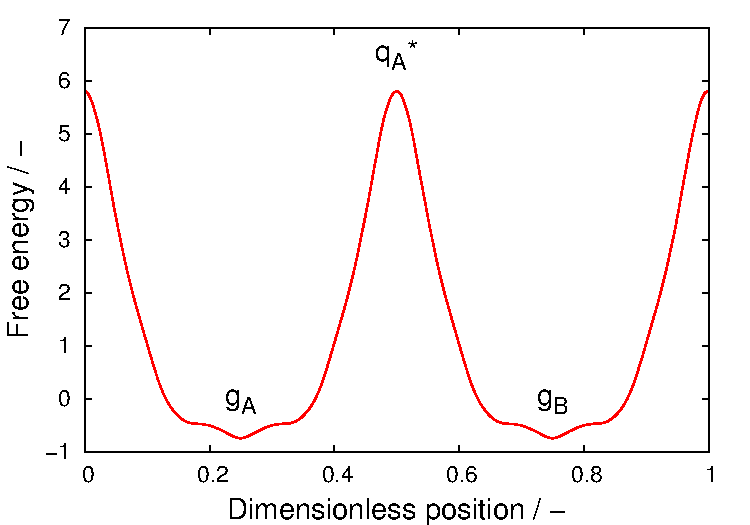
\includegraphics[width=7.5cm]{./Examples/Figures/Umbrella/BiasingProfile/BiasingSpline.pdf}}
  \subfloat[]{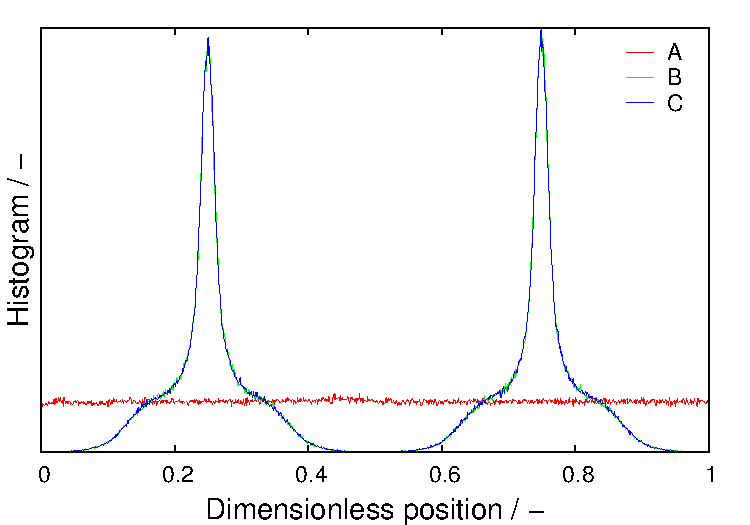
\includegraphics[width=7.5cm]{./Examples/Figures/Umbrella/Histogram/UmbrellaHistogram.pdf}}
  \caption{Umbrella sampling: (a) free energy profile from Widom insertion (the inverse will be used as a biasing potential),
           (b) the histograms of the position of the tagged particle in the direction A (biasing direction), B, and C.}
  \label{Fig: umbrealla sampling}
\end{figure}

\begin{tiny}
\begin{verbatim}
SimulationType                   MonteCarlo
NumberOfCycles                   10000000000
NumberOfInitializationCycles     1000
PrintEvery                       5000

Forcefield                       ExampleZeolitesForceField

Framework                        0
FrameworkName                    LTA_SI
ShiftUnitCells                   0.0 0.0 0.0
UnitCells                        1 1 1
ExternalTemperature              600.0

ComputePositionHistogram         yes
WritePositionHistogramEvery      10000

component 0 MoleculeName                     methane
            MoleculeDefinition               ExampleDefinitions
            BiasingProfile                   Profile.dat
            BiasingMethod                    Umbrella
            BiasingDirection                 A
            BlockPockets                     yes
            BlockPocketsFileName             LTA_SI
            TranslationProbability           1.0
            RotationProbability              1.0
            ReinsertionProbability           1.0
            CreateNumberOfMolecules          1

component 1 MoleculeName                     methane
            MoleculeDefinition               ExampleDefinitions
            BlockPockets                     yes
            BlockPocketsFileName             LTA_SI
            TranslationProbability           1.0
            RotationProbability              1.0
            ReinsertionProbability           1.0
            CreateNumberOfMolecules          31
\end{verbatim}
\end{tiny}

The biasing spline (here called 'Profile.dat') has a header describing the spline:
\begin{tiny}
\begin{verbatim}
# 1801
# 0.5
# 0.25 0.75 12.2775
# 0.0  0.5
0 5.87638 0.0919053
0.000555556 5.79087 0.0924271
...
\end{verbatim}
\end{tiny}
The lines have the following meaning:
\begin{itemize}
\item{the number of data points in the file},
\item{the dimensionless position of the barrier $q^*_A$}
\item{the dimensionless position of the minimum of the free energy $g_A$ and $g_B$, and the distance $d$ between $g_A$ and $g_B$ in Angstrom}
\item{the left and right boundary of $g_A$}
\end{itemize}
followed by the actual data points: 
\begin{itemize}
\item{dimensionless position}
\item{dimensionless free energy $\beta F$ or $F$ in unit of $k_BT$}
\item{error in the free energy}
\end{itemize}


\subsection*{Example 18: dcTST diffusivities}

The first step for dcTST is to compute the free energy profile as a function of a one-dimensional reaction coordinate.
In general this mapping is complex, but for certain zeolites the mapping is trivial.
As an example, we use the LTA-type zeolite with a cubic unit cell of 24.555 \AA.
For this structure, the mapping can be done in $x$, $y$, or $z$ and all three give identical results.
We can define a reaction coordinate from $x=0$ to $x=1$ with several key values:
\begin{itemize}
 \item{x=0}:\quad the window on the left.
 \item{x=0.25}\quad the center of the left cage $A$.
 \item{x=0.5}:\quad the window in the middle separating the left cage $A$ from the right cage $B$.
 \item{x=0.75}\quad the center of the right cage $A$.
 \item{x=1}:\quad the window on the right.
\end{itemize}

\begin{figure}[t]
  \centering
  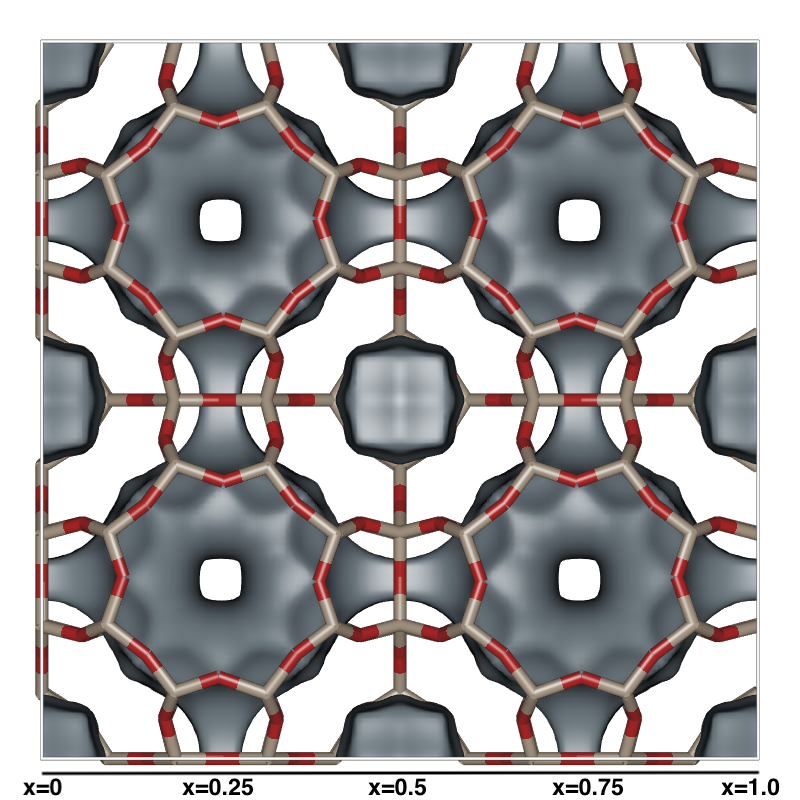
\includegraphics[width=7.5cm]{./Examples/Figures/LTA_dcTST.png}
  \caption{The reaction coordinate mapping for the LTA-type structure.}
  \label{Fig: LTA dcTST}
\end{figure}

\subsubsection{Computing the free energy profile}

The first step is to compute the free energy profile.
A convenient way at low loading is to use Widom insertion.

\begin{tiny}
\begin{verbatim}
SimulationType                   MonteCarlo
NumberOfCycles                   1000000000000000
NumberOfInitializationCycles     1000
PrintEvery                       10000

Forcefield                       ExampleZeolitesForceField

Framework                        0
FrameworkName                    LTA_SI
RemoveAtomNumberCodeFromLabel    yes
ShiftUnitCells                   0.0 0.0 0.0
UnitCells                        1 1 1
ExternalTemperature              600.0

WriteFreeEnergyProfileEvery      5000

component 0 MoleculeName                     methane
            MoleculeDefinition               ExampleDefinitions
            ComputeFreeEnergyProfile         yes
            BlockPockets                     yes
            BlockPocketsFileName             LTA_SI
            TranslationProbability           1.0
            RotationProbability              1.0
            ReinsertionProbability           1.0
            CreateNumberOfMolecules          0
\end{verbatim}
\end{tiny}

The result converge slowly to a nice profile. The scatter is the highest at places where the free energy is high, and
the scatter in the data is low at places of low free energy. We can now define the diffusion in terms of
figure \ref{Fig: LTA Widom}: we compute the diffusion of a molecule from $g_A$ in cage $A$ to $g_B$ in cage $B$
across barrier $q_A^*$.
To input this information we make a "biasing profile"-file (\verb+Profile.dat+) with this data at the top
\begin{small}
\begin{verbatim}
# 1801
# 0.5
# 0.25 0.75 12.2775
# 0.0  0.5
......
\end{verbatim}
\end{small}
First line is the number of data points (here 1801), then the position of the barrier $q_A^*$ (here 0.5),
then $g_A$, $g_B$, and the distance in Angstrom between them (here 0.25, 0.75, and 12.2775, respectively).
and lastly the range of cage $A$ (here from 0.0 to 0.5).

\subsubsection{Computing TST-estimates}

We can now use this file
\begin{verbatim}
  BiasingProfile                   Profile.dat
  BiasingMethod                    Umbrella
  BiasingDirection                 A
\end{verbatim}
to for example perform Umbrella sampling. In addition, it will create a spline-file
\verb+BiasingSpline_methane_0.dat+, that contains a lot of information and a fitting spline.
\begin{small}
\begin{verbatim}
# Dividing surfaces:     0.500000000000 [-]
# Free energy minima:     0.250000000000 [-]     0.750000000000 [-]  lattice distance:    12.277500000000 [A]
# Left and right boundary:     0.000000000000 [-]     0.500000000000 [-]
# F(QstarA):     5.794749230708
# Exp(-Beta QStarA):   0.00304349354572
# Integral Exp(-Beta q) over region left boundary (0) to q* (0.5):  1.10187629401e-09
# Mass reaction bead:    16.042460000000 [au]
# |v|=Sqrt(k_B T/(2.0*PI*Mass)):   222.467902978164 [m/s]
# P(q*) dq:      2762100.93845 [1/m]
# k^TST= |v| P(q*) dq, i.e. the TST hopping rate:       614478803.59 [1/s]
# D^TST:  9.26246952572e-10 [m^2/s]

# RM Int1, Integral Exp(Beta q) over region gA to gB:    18.077489357418
# RM Int2, Integral Exp(-Beta q) over full region:     0.448738054981
# RM Int1*Int2:     8.112057413187
# RM 1/(Int1*Int2):     0.123273289261

# <n_A>:    24.555000000000
# 1/<n_A>:     0.040724903278
\end{verbatim}
\end{small}
It uses the computed smoothed spline that fits the data to calculate the integrals and dcTST information.
The $k^\text{TST}$ is 614478803.59 events per second, and $D^\text{TST}=9.26246952572e-10$ m$^2$/s.
The spline (column 1 and 2) is convenient as it is continuous and smooth.

\begin{figure}[t]
  \centering
  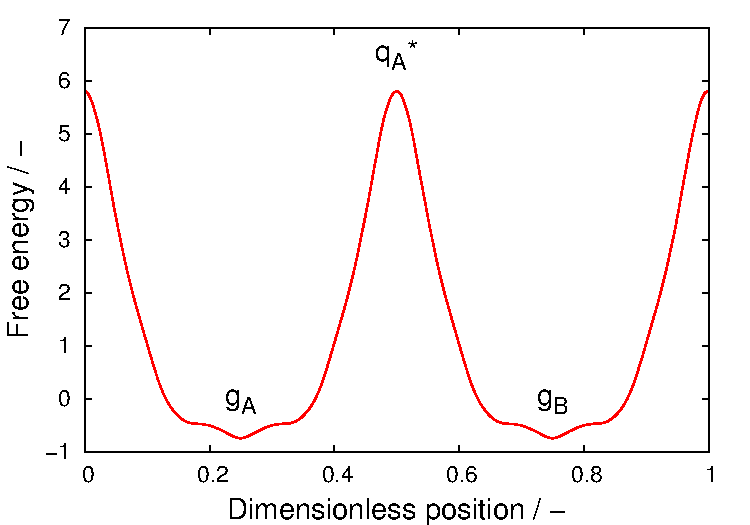
\includegraphics[width=7.5cm]{./Examples/Figures/Umbrella/BiasingProfile/BiasingSpline.pdf}
  \caption{The free energy obtained with Widom insertion.}
  \label{Fig: LTA Widom}
\end{figure}

\subsubsection{Computing free energies at finite loading with brute-force MD}

Of course, one can try to compute the free energy using brute-force MD, for example at an average of 8 molecules per cage.
\begin{tiny}
\begin{verbatim}
SimulationType                   MD
NumberOfCycles                   100000000
NumberOfInitializationCycles     5000
NumberOfEquilibrationCycles      10000
PrintEvery                       10000

Forcefield                       ExampleZeolitesForceField

Framework                        0
FrameworkName                    LTA_SI
RemoveAtomNumberCodeFromLabel    yes
ShiftUnitCells                   0.0 0.0 0.0
UnitCells                        1 1 1
ExternalTemperature              600.0

ComputePositionHistogram         yes
WritePositionHistogramEvery      10000

component 0 MoleculeName                     methane
            MoleculeDefinition               ExampleDefinitions
            BlockPockets                     yes
            BlockPocketsFileName             LTA_SI
            TranslationProbability           1.0
            RotationProbability              1.0
            ReinsertionProbability           1.0
            CreateNumberOfMolecules          64
\end{verbatim}
\end{tiny}

However, this only works for low free energy barriers.

\subsubsection{Computing free energies at finite loading using Umbrella sampling}

With Umbrella sampling we can bias the movement of a single tagged molecule at the proper chosen loading.
We therefore need two components: component one is a single biased molecule, and component two are the
other (unbiased) particles.
We can compute the histogram of the positions and for component one, recomputed the actual free energy
taking the biasing into account.

\begin{tiny}
\begin{verbatim}
SimulationType                   MonteCarlo
NumberOfCycles                   1000000000000000
NumberOfInitializationCycles     1000
PrintEvery                       1000

Forcefield                       ExampleZeolitesForceField

Framework                        0
FrameworkName                    LTA_SI
ShiftUnitCells                   0.0 0.0 0.0
UnitCells                        1 1 1
ExternalTemperature              600.0

ComputePositionHistogram         yes
WritePositionHistogramEvery      10000

component 0 MoleculeName                     methane
            MoleculeDefinition               ExampleDefinitions
            BiasingProfile                   Profile.dat
            BiasingMethod                    Umbrella
            BiasingDirection                 A
            BlockPockets                     yes
            BlockPocketsFileName             LTA_SI
            TranslationProbability           1.0
            RotationProbability              1.0
            ReinsertionProbability           1.0
            CreateNumberOfMolecules          1

component 1 MoleculeName                     methane
            MoleculeDefinition               ExampleDefinitions
            BlockPockets                     yes
            BlockPocketsFileName             LTA_SI
            TranslationProbability           1.0
            RotationProbability              1.0
            ReinsertionProbability           1.0
            CreateNumberOfMolecules          63
\end{verbatim}
\end{tiny}

\subsubsection{Computing the dynamical correction}

The TST estimates are \dots estimates. In reality, not all particles at the dividing surface actually cross
the boundary. We have to explicitly compute this property using many short MD trajectories.
Step one is to compute initial state for these trajectories:
\begin{tiny}
\begin{verbatim}
SimulationType                   MonteCarlo
NumberOfCycles                   100000000
NumberOfInitializationCycles     1000
PrintEvery                       100

Forcefield                       ExampleZeolitesForceField

Framework                        0
FrameworkName                    LTA_SI
RemoveAtomNumberCodeFromLabel    yes
ShiftUnitCells                   0.0 0.0 0.0
UnitCells                        1 1 1
ExternalTemperature              600.0

WritedcTSTSnapShotsToFile        yes
PutMoleculeOnBarrier             yes
BarrierPosition                  0.5 0.25 0.25
WritedcTSTSnapShotsEvery         100


component 0 MoleculeName                     methane
            MoleculeDefinition               ExampleDefinitions
            TranslationProbability           1.0
              TranslationDirection             bc
            RotationProbability              1.0
            RegrowInPlaceProbability         1.0
            CreateNumberOfMolecules          0

component 1 MoleculeName                     methane
            MoleculeDefinition               ExampleDefinitions
            ComputeFreeEnergyProfile         yes
            BlockPockets                     yes
            BlockPocketsFileName             LTA_SI
            TranslationProbability           1.0
            RotationProbability              1.0
            ReinsertionProbability           1.0
            CreateNumberOfMolecules          63
\end{verbatim}
\end{tiny}

To sample configurations, we need to write out "snapshots", but with some sampling in between to diminish the
correlation between the snapshots. We also need to place the particle at the barrier and define the barrier position.

\begin{small}
\begin{verbatim}
  WritedcTSTSnapShotsToFile        yes
  PutMoleculeOnBarrier             yes
  BarrierPosition                  0.5 0.25 0.25
  WritedcTSTSnapShotsEvery         100
\end{verbatim}
\end{small}
Also note, that the particle on the barrier is restricted to only move one the barrier plane.
\begin{small}
\begin{verbatim}
  TranslationProbability           1.0
  TranslationDirection             bc
\end{verbatim}
\end{small}

We can do uses the sampled snapshots to run many barrier-recrossing MD trajectories.
\begin{small}
\begin{verbatim}
SimulationType                   BarrierRecrossing
  
Forcefield                       ExampleZeolitesForceField

Framework                        0
FrameworkName                    LTA_SI
RemoveAtomNumberCodeFromLabel    yes
ShiftUnitCells                   0.0 0.0 0.0
UnitCells                        1 1 1
ExternalTemperature              600.0

PutMoleculeOnBarrier             yes
FreeEnergyMappingType            A
BarrierPosition                  0.5 0.25 0.25
MaxBarrierDistance               4.0
MaxBarrierTime                   10.0
NumberOfVelocities               1

component 0 MoleculeName                     methane
            MoleculeDefinition               ExampleDefinitions
            CreateNumberOfMolecules          0

component 1 MoleculeName                     methane
            MoleculeDefinition               ExampleDefinitions
            CreateNumberOfMolecules          63
\end{verbatim}
\end{small}

\section{Auxiliary examples}

\subsection*{Example 1: Computing the ideal gas Rosenbluth weights of linear alkanes C$_5$ - C$_9$}

To compare simulation values to experiments a reference state should be chosen. A convenient reference state
is the ideal gas. The reference Rosenbluth value can be computed from a simulation of a single chain at the
desired temperature. Note that for Rosenbluth weights several chains can be computed simultaneously, since
they are computed from Widom insertions where the molecule is never actually inserted in the system.

\begin{tiny}
\begin{verbatim}
SimulationType        MonteCarlo
NumberOfCycles        25000
PrintEvery            1000
PrintPropertiesEvery  1000

Forcefield            ExampleZeolitesForceField

Box 0
BoxLengths 30 30 30
ExternalTemperature 573.0

Component 0 MoleculeName              pentane
            MoleculeDefinition        ExampleDefinitions
            WidomProbability          1.0
            CreateNumberOfMolecules   0

Component 1 MoleculeName              hexane
            MoleculeDefinition        ExampleDefinitions
            WidomProbability          1.0
            CreateNumberOfMolecules   0

Component 2 MoleculeName              heptane
            MoleculeDefinition        ExampleDefinitions
            WidomProbability          1.0
            CreateNumberOfMolecules   0

Component 3 MoleculeName              octane
            MoleculeDefinition        ExampleDefinitions
            WidomProbability          1.0
            CreateNumberOfMolecules   0

Component 4 MoleculeName              nonane
            MoleculeDefinition        ExampleDefinitions
            WidomProbability          1.0
            CreateNumberOfMolecules   0
\end{verbatim}
\end{tiny}
\noindent
The output contains 
\begin{tiny}
\begin{verbatim}
     Average Widom Rosenbluth factor:
     ================================
             [C5] Average Widom:   0.0668555 +/- 0.000131 [-]
             [C6] Average Widom:   0.0175062 +/- 0.000067 [-]
             [C7] Average Widom:   0.00462547 +/- 0.000010 [-]
             [C8] Average Widom:   0.00122842 +/- 0.000005 [-]
             [C9] Average Widom:   0.000328228 +/- 0.000001 [-]
\end{verbatim}
\end{tiny}
which is printed every `PrintPropertiesEvery' cycles. The `Rosenbluth factor new' are the values of interest.
The average and error estimated from block averages is printed at the end
of the simulation.

\subsection*{Example 2: Computing the ideal gas Rosenbluth weights of hexane isomers}

\begin{tiny}
\begin{verbatim}
     SimulationType        MonteCarlo
     NumberOfCycles        25000
     PrintEvery            1000
     PrintPropertiesEvery  1000
     
     Forcefield            ExampleZeolitesForceField
     
     Box 0
     BoxLengths 30 30 30
     ExternalTemperature 433.0
     
     Component 0 MoleculeName              hexane
                 MoleculeDefinition        ExampleDefinitions
                 WidomProbability          1.0
                 CreateNumberOfMolecules   0
     
     Component 1 MoleculeName              2-methylpentane
                 MoleculeDefinition        ExampleDefinitions
                 WidomProbability          1.0
                 CreateNumberOfMolecules   0
     
     Component 2 MoleculeName              3-methylpentane
                 MoleculeDefinition        ExampleDefinitions
                 WidomProbability          1.0
                 CreateNumberOfMolecules   0
     
     Component 3 MoleculeName              22-dimethylbutane
                 MoleculeDefinition        ExampleDefinitions
                 WidomProbability          1.0
                 CreateNumberOfMolecules   0
\end{verbatim}
\end{tiny}

\subsection*{Example 3: Computing the helium void-fraction of a structure (pore volume)}

The void fraction is the empty space of a structure divided by the total volume. In experiment it
is measured using helium, because helium does (almost) not adsorb. It would be consistent to also
measure this fraction using helium at room temperature. In practice it is easily computed from
Widom particle insertion as the void fraction corresponds to the new Rosenbluth weight.
\begin{tiny}
\begin{verbatim}
     SimulationType        MonteCarlo
     NumberOfCycles        500000
     PrintEvery            10000
     PrintPropertiesEvery  10000
     
     Forcefield            ExampleMOFsForceField
     
     Framework 0
     FrameworkName IRMOF-1
     UnitCells 1 1 1
     ExternalTemperature 298.0
     
     Component 0 MoleculeName             helium
                 MoleculeDefinition       ExampleDefinitions
                 WidomProbability         1.0
                 CreateNumberOfMolecules  0
\end{verbatim}
\end{tiny}

The Rosenbluth weight, and therefore the helium void fraction of IRMOF-1 is approximately 0.80.
The pore volume is the void fraction times the unit cell volume. Note that the values dependent
slightly on the cutoff, and shifted vs. truncated potentials.
\begin{tiny}
\begin{verbatim}
     Average Widom Rosenbluth factor:
     ================================
             Block[ 0] 0.803749 [-]
             Block[ 1] 0.803741 [-]
             Block[ 2] 0.803497 [-]
             Block[ 3] 0.803818 [-]
             Block[ 4] 0.803536 [-]
             ------------------------------------------------------------------------------
             [helium] Average Widom:   0.803668 +/- 0.000255 [-]
\end{verbatim}
\end{tiny}

\subsection*{Example 4: Computing the surface area of IRMOF-1}

The geometric surface area can easily be computed by `rolling an atom over the surface' and measure the surface. In practice,
for each framework atom points are generate on a sphere around the framework atom, and the amount of overlap with other framework
atoms is determined. The fraction of overlap is multiplied times the area of the sphere. The summation over all framework atoms
gives the geometric surface area. This example shows how to compute the surface area of IRMOF-1. `SurfaceAreaSamplingPointsPerShere'
is the amount of points generated on sphere at a distance dependent on the mixing rule, the probe-atom and the current framework atom type.
The more points the higher the accuracy. The simulation usually takes between 5 and 30 minutes.

In this example the structure is probed with hydrogen using the second bead (`H\_com' with $\sigma=2.958$ \AA). The option
`SurfaceAreaProbeDistance Sigma' sets the overlap criteria to $\sigma$ instead of the default $\sigma^{1/6}$.

\begin{tiny}
\begin{verbatim}
     SimulationType        MonteCarlo
     NumberOfCycles        10000
     PrintEvery            100
     PrintPropertiesEvery  100
     
     Forcefield Dubbeldam2007FlexibleIRMOF-1
     CutOff 12.8
     
     Framework 0
     FrameworkName IRMOF-1
     UnitCells 1 1 1
     SurfaceAreaProbeDistance Sigma
     
     Component 0 MoleculeName             argon
                 MoleculeDefinition       ExampleDefinitions
                 SurfaceAreaProbability   1.0
                 CreateNumberOfMolecules  0
\end{verbatim}
\end{tiny}
The area depends on the probe atom and on whether the well-depth at $2^{1/6}\sigma$ ($\approx 1.12246\sigma$)
is used (`SurfaceAreaProbeDistance Minimum')
\begin{tiny}
\begin{verbatim}
     Surface area: 2082.509853 [m^2/cm^3]
     Surface area: 3510.189484 [m^2/g]
\end{verbatim}
\end{tiny}
or $\sigma$ is used as the distance criteria (`SurfaceAreaProbeDistance Sigma'):
\begin{tiny}
\begin{verbatim}
     Surface area: 2266.243128 [m^2/cm^3]
     Surface area: 3819.882429 [m^2/g]
\end{verbatim}
\end{tiny}


\subsection*{Example 5: Powder diffraction pattern}

Powder diffraction is a scientific technique using X-Ray or neutron diffraction on powder or microcrystalline samples
for structural characterization of materials.
The most widespread use of powder diffraction is in the identification and characterization of crystalline solids,
each of which produces a distinctive diffraction pattern. Both the positions (corresponding to lattice spacings) and
the relative intensity of the lines are indicative of a particular phase and material, providing a "fingerprint" for comparison.
The database of IZA for zeolite has the option to generate the powder diffraction pattern:
\begin{tiny}
\begin{verbatim}
     http://izasc.ethz.ch/fmi/xsl/IZA-SC/xrd.xsl
\end{verbatim}
\end{tiny}

Here, an example of the powder diffraction pattern for the TON-type zeolite. Only one unit cell is sufficient for the computation
(interactions are not needed in the computation, just the position and types of the atoms and the shape and size of the unit cell).
The diffraction pattern usually takes a few seconds of computation, and the result is written to `PowderDiffraction/System[0]/'. It contains
two files: `PeakInformation.dat' and `Spectrum.dat'.
\begin{tiny}
\begin{verbatim}
     SimulationType  MonteCarlo
     NumberOfCycles  0
     
     Forcefield      ExampleZeolitesForceField
     
     Framework 0
     FrameworkName TON
     UnitCells 1 1 1
     
     ComputePowderDiffractionPattern yes
     DiffractionType Xray
     DiffractionRadiationType Copper
     WaveLengthType single
     TwoThetaMin 1
     TwoThetaMax 50
     TwoThetaStep 0.02
     PeakShape PseudoVoigt
     PeakWidthModifierU 0.005
\end{verbatim}
\end{tiny}

The first elements of the file `PeakInformation.dat' look like:
\begin{tiny}
\begin{verbatim}
     # 2-theta   d         h  k  l  Mult Lp          Scat. Factor    Intensity
       8.15213   0.09220 [ 1, 1, 0]    4 392.85927   19014.2044440544   100.000000
      10.15550   0.11481 [ 0,-2, 0]    2 252.33302   12381.2641234081    20.911920
      12.77464   0.14431 [ 2, 0, 0]    2 158.63285   19714.5657150741    20.933178
      16.34589   0.18441 [ 2, 2, 0]    4  96.01738    6730.9888808237     8.651941
      16.55216   0.18672 [-1,-3, 0]    4  93.58434     739.8429009358     0.926889
      19.42690   0.21886 [-1,-1,-1]    4  67.33674    3040.0925085839     2.740461
      .......................................
\end{verbatim}
\end{tiny}
So, the elements are the angle $2\theta$, the $d$-spacing, the Miller indices $h$,$k$, and $l$, the multiplicity,
the Lorentz-Polarization factor, the scattering factor (including anomalous scattering), and the relative intensity (where
the largest intensity is set to 100).
The second file `Spectrum.dat' can be plotted using gnuplot, the first column is $2\theta$, the second column the intensity.
The shape of the peaks can be influenced with `PeakShape', and the peak width modifiers `PeakWidthModifierU',
`PeakWidthModifierV', and `PeakWidthModifierW'.

\subsection*{Example 6: Making `grids'}

For rigid frameworks one can precompute the energy-grid, because the potential energy field induces by the framework does
not evolve in time. For each of the pseudo atoms one can generate a 3D grid where the spacing can be defined. In the example
the grid points are 0.1 \AA\ spaced apart (a=b=c=25.832\AA, $258\times258\times258=17173512$ points). 
A shorter distance results in more points, more accuracy, but also a bigger
grid (more memory is needed). Note that RASPA can handle a `mixture' of grids and fully computed interactions.
The table stores $U,\frac{\partial U}{\partial x}$, $\frac{\partial U}{\partial y}$, $\frac{\partial U}{\partial z}$,
$\frac{\partial^2 U}{\partial x\partial y}$, $\frac{\partial^2 U}{\partial x\partial z}$, $\frac{\partial^2 U}{\partial y\partial z}$,
and $\frac{\partial^3 U}{\partial x\partial y \partial z}$ at each grid point. The interpolation can handle non-orthorhombic cells
and can also be used for molecular dynamics (i.e. the force interpolation is consistent with the energy interpolation).

\begin{tiny}
\begin{verbatim}
     SimulationType  MakeGrid

     Forcefield      FlexibleIRMOF-1

     Framework 0
     FrameworkName IRMOF-1
     UnitCells 1 1 1

     NumberOfGrids 2
     GridTypes C_co2 O_co2
     SpacingVDWGrid 0.1
     SpacingCoulombGrid 0.1
\end{verbatim}
\end{tiny}

\subsection*{Example 7: Using `grids'}

\noindent The grids are stored in `/share/raspa/grids/FlexibleIRMOF-1/IRMOF-1/0.100000' and the names are
`IRMOF-1\_C\_co2\_shifted.grid', `IRMOF-1\_O\_co2\_shifted.grid', and `IRMOF-1\_Electrostatics\_Ewald.grid'.
The last grid is the real part of the Ewald summation, i.e. erfc(r)/r using a probe charge of +1.
They can be used like:
\begin{tiny}
\begin{verbatim}
     SimulationType                MonteCarlo
     NumberOfCycles                5000
     NumberOfInitializationCycles  5000
     PrintEvery                    100

     Forcefield                    FlexibleIRMOF-1
     ChargeMethod                  Ewald
     EwaldPrecision                1e-6

     Framework 0
     FrameworkName IRMOF-1
     UnitCells 1 1 1
     ExternalTemperature 298.0
     ExternalPressure 5000000.0

     NumberOfGrids 2
     GridTypes C_co2 O_co2
     SpacingVDWGrid 0.1
     SpacingCoulombGrid 0.1
     UseTabularGrid yes

     Component 0 MoleculeName                     CO2
                 MoleculeDefinition               ExampleDefinitions
                 TranslationProbability           1.0
                 RotationProbability              1.0
                 ReinsertionProbability           1.0
                 SwapProbability                  1.0
                 CreateNumberOfMolecules          0
\end{verbatim}
\end{tiny}
In the output file, in the framework section, the used grids are tested one by one.
Make sure the relative error is smaller than about 0.001 for the energies. 
If not, either the wrong grid is used (the current settings for the force field, cutoff etc. are different from what the grid has been made with)
or the structure requires a higher interpolation density.
\begin{tiny}
\begin{verbatim}
     PseudoAtom 9 Framework-[C_co2]
     =========================================================================================
         Boltzmann average energy VDW (table)                 :  -166.674268647739
         Boltzmann average energy VDW (full)                  :  -166.672515492945
         Boltzmann relative error VDW                         :     0.000050342536
         Boltzmann average energy Coulomb (table)             :  -132.261348754564
         Boltzmann average energy Coulomb (full)              :  -132.258792721618
         Boltzmann relative error Coulomb                     :     0.000048335817
     =========================================================================================
         Boltzmann average Force[x] VDW (table)               :     2.814676235131
         Boltzmann average Force[x] VDW (full)                :     2.813903005890
         Boltzmann relative error VDW                         :     0.000679313669
         Boltzmann average Force[x] Coulomb (table)           :    -6.914879772888
         Boltzmann average Force[x] Coulomb (full)            :    -6.906268341227
         Boltzmann relative error Coulomb                     :     0.001165040569
     =========================================================================================
         Boltzmann average Force[y] VDW (table)               :     5.650590778180
         Boltzmann average Force[y] VDW (full)                :     5.646815005685
         Boltzmann relative error VDW                         :     0.000625049225
         Boltzmann average Force[y] Coulomb (table)           :    -6.131228972874
         Boltzmann average Force[y] Coulomb (full)            :    -6.143469499297
         Boltzmann relative error Coulomb                     :     0.001198288617
     =========================================================================================
         Boltzmann average Force[z] VDW (table)               :    -7.613158899110
         Boltzmann average Force[z] VDW (full)                :    -7.613093463878
         Boltzmann relative error VDW                         :     0.000638624417
         Boltzmann average Force[z] Coulomb (table)           :    -5.277718273766
         Boltzmann average Force[z] Coulomb (full)            :    -5.272042035095
         Boltzmann relative error Coulomb                     :     0.001211372128
     
     
     PseudoAtom 10 Framework-[O_co2]
     =========================================================================================
         Boltzmann average energy VDW (table)                 :  -385.683245095266
         Boltzmann average energy VDW (full)                  :  -385.679393087921
         Boltzmann relative error VDW                         :     0.000023203661
         Boltzmann average energy Coulomb (table)             :    92.387158042874
         Boltzmann average energy Coulomb (full)              :    92.385385971036
         Boltzmann relative error Coulomb                     :     0.000049328766
     =========================================================================================
         Boltzmann average Force[x] VDW (table)               :   -12.358055145720
         Boltzmann average Force[x] VDW (full)                :   -12.364288510033
         Boltzmann relative error VDW                         :     0.000522114664
         Boltzmann average Force[x] Coulomb (table)           :    -1.639803867255
         Boltzmann average Force[x] Coulomb (full)            :    -1.640207574883
         Boltzmann relative error Coulomb                     :     0.001302056759
     =========================================================================================
         Boltzmann average Force[y] VDW (table)               :    -3.248927867445
         Boltzmann average Force[y] VDW (full)                :    -3.245131932968
         Boltzmann relative error VDW                         :     0.000521447609
         Boltzmann average Force[y] Coulomb (table)           :    -3.993441639796
         Boltzmann average Force[y] Coulomb (full)            :    -3.990850472425
         Boltzmann relative error Coulomb                     :     0.001252842918
     =========================================================================================
         Boltzmann average Force[z] VDW (table)               :     7.195354496737
         Boltzmann average Force[z] VDW (full)                :     7.193452593912
         Boltzmann relative error VDW                         :     0.000556132560
         Boltzmann average Force[z] Coulomb (table)           :     1.773911985304
         Boltzmann average Force[z] Coulomb (full)            :     1.774122551801
         Boltzmann relative error Coulomb                     :     0.001236592291
\end{verbatim}
\end{tiny}

\subsection*{Example 8: Charge-equilibrium IRMOF-1}

\begin{tiny}
\begin{verbatim}
SimulationType                   MonteCarlo
NumberOfCycles                   0
NumberOfInitializationCycles     0
PrintEvery                       100
RestartFile                      no

Forcefield                       ExampleMOFsForceField
CutOff                           12.0

ChargeFromChargeEquilibration    yes
ChargeEquilibrationPeriodic      yes
ChargeEquilibrationEwald         yes
SymmetrizeFrameworkCharges       no

Framework           0
FrameworkName       IRMOF-1
UnitCells           1 1 1
ExternalTemperature 298.0
ExternalPressure    0.0
\end{verbatim}
\end{tiny}

\subsection*{Example 9: Pore-Size Distribution}

\begin{tiny}
\begin{verbatim}
SimulationType                   PSD
NumberOfCycles                   10000
NumberOfInitializationCycles     0
PrintEvery                       10

ChargeMethod                     Ewald
CutOff                           12.0
Forcefield                       ExampleMOFsForceField
EwaldPrecision                   1e-6

Framework                        0
FrameworkName                    IRMOF-1
UnitCells                        1 1 1
ExternalTemperature              300.0
PSDProbeDistance                 Sigma
WritePSDHistogramEvery           100
PSDHistogramSize                 1000
PSDRange                         10.0
\end{verbatim}
\end{tiny}

\subsection*{Example 10: Typing framework atoms}

\begin{tiny}
\begin{verbatim}
     SimulationType                   MonteCarlo
     NumberOfCycles                   0
     
     Forcefield                       Local
     
     Framework 0
     FrameworkName NU-100SP
     UnitCells 1 1 1
     ExternalTemperature 298.0
     
     ModifyFrameworkAtomConnectedTo C C1 O
     ModifyFrameworkAtomConnectedTo C C2 C1
     ModifyFrameworkAtomConnectedTo C C3 C2 C2
     ModifyFrameworkAtomConnectedTo C C4 C2
     ModifyFrameworkAtomConnectedTo C C5 C4
     ModifyFrameworkAtomConnectedTo C C6 C5
     ModifyFrameworkAtomConnectedTo C C7 C6
     ModifyFrameworkAtomConnectedTo C C8 C7
     ModifyFrameworkAtomConnectedTo C C9 C8
     ModifyFrameworkAtomConnectedTo C C10 C9
     ModifyFrameworkAtomConnectedTo C C11 C10
     ModifyFrameworkAtomConnectedTo C C12 C11
     ModifyFrameworkAtomConnectedTo C C13 C12
     ModifyFrameworkAtomConnectedTo C C14 C13
     ModifyFrameworkAtomConnectedTo C C15 C14
     ModifyFrameworkAtomConnectedTo H H1 C3
     ModifyFrameworkAtomConnectedTo H H2 C4
     ModifyFrameworkAtomConnectedTo H H3 C9
     ModifyFrameworkAtomConnectedTo H H4 C10
     ModifyFrameworkAtomConnectedTo H H5 C15
     ModifyFrameworkAtomConnectedTo O O2 C1
     ModifyFrameworkAtomConnectedTo Cu Cu O2
\end{verbatim}
\end{tiny}

\subsection*{Example 11: Random Aluminum Distribution}

The Nax structure is defined in the CIF-file as
\begin{tiny}
\begin{verbatim}
     loop_
     _atom_site_label
     _atom_site_type_symbol
     _atom_site_fract_x
     _atom_site_fract_y
     _atom_site_fract_z
     _atom_site_charge
     Si1      Si4+  -0.05381   0.12565   0.03508   2.05
     Al1      Al3+  -0.05524   0.03639   0.12418   1.75
     O1       O2-   -0.1099    0.0003    0.1056   -1.025
     O2       O2-   -0.0011   -0.0028    0.1416   -1.025
     O3       O2-   -0.0346    0.0758    0.0711   -1.025
     O4       O2-   -0.0693    0.0726    0.18     -1.025
     Oa1      O2-    ?         ?         ?        -1.2
     Oa2      O2-    ?         ?         ?        -1.2
     Oa3      O2-    ?         ?         ?        -1.2
     Oa4      O2-    ?         ?         ?        -1.2
\end{verbatim}
\end{tiny}
The atom-types found in the cif-file, and not already defined in the \verb+Pseudo_atoms.def+-file, will be automatically added.
The \verb+Oa1+, \verb+Oa2+, \verb+Oa3+, and \verb+Oa4+ atoms are added but have no defined positions.
The initial structure has the maximum amount of aluminum (given the Lowenstein rule)
\begin{tiny}
\begin{verbatim}
     Pseudo Atoms    8 [     Si1]:   96 atoms
     Pseudo Atoms    9 [     Al1]:   96 atoms
     Pseudo Atoms   10 [      O1]:   96 atoms
     Pseudo Atoms   11 [      O2]:   96 atoms
     Pseudo Atoms   12 [      O3]:   96 atoms
     Pseudo Atoms   13 [      O4]:   96 atoms
\end{verbatim}
\end{tiny}
To create a NaY version with 58 aluminum we can take 38 aluminum randomly and change them to silicon.
We also modify the \verb+O1+-\verb+O4+ to types \verb+Oa1+-\verb+Oa4+ when connected to an aluminum.
\begin{tiny}
\begin{verbatim}
     SimulationType                MC
     NumberOfCycles                0
     NumberOfInitializationCycles  0
     PrintEvery                    10
     
     Forcefield                    Local
     
     RandomlySubstitute 38 Al1 Si1
     
     ModifyFrameworkAtomConnectedTo O1 Oa1 Al1
     ModifyFrameworkAtomConnectedTo O2 Oa2 Al1
     ModifyFrameworkAtomConnectedTo O3 Oa3 Al1
     ModifyFrameworkAtomConnectedTo O4 Oa4 Al1
     
     Framework 0
     FrameworkName NaX
     UnitCells 1 1 1
     ExternalTemperature 300.0
\end{verbatim}
\end{tiny}
The new structure can be found in the \verb+Movie+ directory and has the desired content
\begin{tiny}
\begin{verbatim}
     Pseudo Atoms    8 [     Si1]:  134 atoms
     Pseudo Atoms    9 [     Al1]:   58 atoms
     Pseudo Atoms   10 [      O1]:   38 atoms
     Pseudo Atoms   11 [      O2]:   38 atoms
     Pseudo Atoms   12 [      O3]:   38 atoms
     Pseudo Atoms   13 [      O4]:   38 atoms
     Pseudo Atoms   14 [     Oa1]:   58 atoms
     Pseudo Atoms   15 [     Oa2]:   58 atoms
     Pseudo Atoms   16 [     Oa3]:   58 atoms
     Pseudo Atoms   17 [     Oa4]:   58 atoms
\end{verbatim}
\end{tiny}

\newpage
\section{Where to go from here?}

\subsection*{Constructing your own input for your systems}

The first thing to do is to scan the scientific literature whether people have already developed models for your system.
The models for small adsorbates by the Calero-group using shifted LJ potentials (cutoff 12 \AA)
for molecules calibrated on experimental vapor-liquid equilibrium data.
These potentials can be used by both MC and MD, which is a great advantage.

\begin{table}[H]
\begin{tabular}{p{5.5cm}|p{1.5cm}|p{1.3cm}|p{1.3cm}|p{1.0cm}|p{1.15cm}|p{1.0cm}|p{1.0cm}}
molecule type &  all-atom & type & $\epsilon/k_B$ [K] & $\sigma$ [\AA] & $q$ [e] & cutoff & shifted\\
\hline
\hline
N$_2$, bond-distance 1.1 \AA \cite{MartinCalvo2011} & yes  & N (N$_2$) & 38.298 & 3.306 & -0.405 & 12 & yes\\
\multicolumn{1}{r|}{(0.55 \AA\ from N atom)}   & -    & Dummy     &        &       & 0.810  & 12 & yes\\
\hline
O$_2$, bond-distance 1.2 \AA \cite{MartinCalvo2011} & yes  & O (O$_2$) & 53.023 & 3.045 & -0.112 & 12 & yes\\
\multicolumn{1}{r|}{(0.6 \AA\ from O atom)}  & -    & Dummy     &        &       & 0.224  & 12 & yes\\
\hline
Ar \cite{MartinCalvo2011} & yes  & Ar & 124.070 & 3.380 & 0.0 & 12 & yes\\
\hline
CCl$_4$  \cite{MartinCalvo2011} & no  & CCl$_4$ & 519.730 & 5.140 & 0.0 & 12 & yes\\
\hline
CO, bond-distance 1.128 \AA  \cite{MartinCalvo2012}  & yes  & C     & 16.141 & 3.636 & -0.2424 & 12 & yes\\
                            & yes  & O     & 98.014 & 2.979 & -0.2744 & 12 & yes\\
\multicolumn{1}{r|}{(0.6443 \AA\ from C atom)}   & -    & Dummy &        &       &  0.5168 & 12 & yes\\
\hline
CO$_2$, bond-distance 1.149 \AA\ \cite{GarciaSanchez2009} & yes  & O     & 85.671 & 3.017 & -0.3256 & 12 & yes\\
                              & yes  & C     & 29.933 & 2.745 & -0.6512 & 12 & yes\\
\hline
SO$_2$, bond-distance 1.431 \AA\ \cite{MatitoMartos2014}  & yes  & S     & 189.353 & 3.41 & 0.402 & 12 & yes\\
\multicolumn{1}{r|}{(bond angle of 119$^\circ$)} & yes  & O     & 58.725 & 3.198 & -0.201 & 12 & yes\\
\hline
SF$_6$, bond-distance 1.565 \AA\ \cite{MatitoMartos2015} & yes  & F     & 73.130 & 2.843 & - & 12 & yes\\
                                & yes  & S     &  - &   - & - & 12 & yes\\
\hline
H2S, bond-distance 1.34 \AA\ \cite{GutierrezSevillano2013} & yes  & S     & 275 & 3.7 & -0.32 & 12 & yes\\
\multicolumn{1}{r|}{(bond angle of 92$^\circ$)}    & yes  & H     & -   & -   &  0.16 & 12 & yes\\
\hline
Alkenes \cite{Liu2008} & no  &       & -   & -   &  -    & 12 & yes\\
\hline
propylene \cite{GutierrezSevillano2010} & no  & CH$_3$  & 93.0 & 3.685 & 0.87 & 12 & yes\\
                   & no  & CH  & 51.0 & 4.0 & 0.87 & 12 & yes\\
\multicolumn{1}{r|}{(Dummy-CH$_2$ bond length 0.704 \AA)} & -   & Dummy &      &     & -1.74 & 12 & yes\\
                   & -   & CH$_3$ & 108.0 & 3.76 & - & 12 & yes\\
\end{tabular}
\caption{Selection of models by the Calero-group using shifted LJ potentials (cutoff 12 \AA)
 for molecules calibrated on experimental vapor-liquid equilibrium data.
 These potentials can be used by both MC and MD.
 Cross terms are computed using Lorentz-Berthelot mixing rules.}
\label{Table: Calero VLE calibrated LJ}
\end{table}
\begin{table}[H]
\begin{tabular}{p{3.5cm}|p{3.5cm}|p{4.0cm}|p{4.0cm}}
molecule type &  framework & cation & reference\\
\hline
\hline
    alkanes     & MOR, MFI & Na     & Beerdsen et al.\cite{Beerdsen2002}\\
    alkanes     & MFI      & Li, Na, K, Cs, Ca, Ba     & Beerdsen et al.\cite{Beerdsen2003}\\
    alkanes     & NaY      & Na  & Calero et al.\cite{Calero2004}\\
    alkanes     & LTA-5A   & Na,Ca  & Garcia-Perez et al.\cite{GarciaPerez2006}\\
    CO$_2$     & LTA-4A   & Na  & Garcia-Sanchez et al.\cite{GarciaSanchez2009}\\
\hline
\end{tabular}
\caption{Selection of models by the Calero-group using shifted LJ potentials (cutoff 12 \AA)
    for molecules in zeolites with cations.}
\label{Table: Calero cations calibrated LJ}
\end{table}

A computational very efficient model is the Transferable potentials for Phase Equilibria  TraPPE force field by Martin and Siepmann\cite{Martin1998,Martin1999}.
The force field describes linear, mono-branched and di-branched alkanes\cite{Martin1998,Martin1999},
benzene, pyridine, pyrimidine, pyrazine, pyridazine, thiophene, furan, pyrrole, thiazole, oxazole, isoxazole, imidazole, and pyrazole\cite{Rai2007},
primary, secondary, and tertiary amines, nitroalkanes and nitrobenzene, nitriles, amides, pyridine, and pyrimidine\cite{Wick2005a},
ethers, glycols, ketones, and aldehydes\cite{Stubbs2004},
thiols, sulfides, disulfides, and thiophene \cite{Lubna2005}, as well as some smaller molecule
like CO$_2$ and N$_2$ \cite{Potoff2001} and ethane and ethylene\cite{Shah2017}.
Despite the fact that the model lumps CH$_3$, CH$_2$, and CH into single interaction centers, it very accurately
reproduces the experimental phase diagram and critical points.
This united atom approach allows for much longer simulation times and larger systems because each of the CH$_x$-groups is
charge-neutral and charge-charge interaction can be omitted.
Some TraPPE models for small molecules are listed in Table \ref{Table: TraPPE VLE calibrated LJ}.

\begin{table}[H]
\begin{tabular}{p{5.5cm}|p{1.5cm}|p{1.3cm}|p{1.3cm}|p{1.0cm}|p{1.15cm}|p{1.0cm}|p{1.0cm}}
molecule type &  all-atom & type & $\epsilon/k_B$ [K] & $\sigma$ [\AA] & $q$ [e] & cutoff & shifted\\
\hline
\hline
Alkanes \cite{Martin1998} & no  & CH$_4$ & 148 & 3.73 & - & 14 & no\\
                         & no  & CH$_3$ & 98 & 3.75 & - & 14 & no\\
                         & no  & CH$_2$ & 46 & 3.95 & - & 14 & no\\
\hline
Branched alkanes\cite {Martin1999} & no  & CH & 10 & 4.68 & - & 14 & no\\
                                  & no  & C & 0.5 & 6.4 & - & 14 & no\\
\hline
CO$_2$, bond-distance 1.16 \AA\ \cite{Potoff2001} & yes  & O     & 79.0 & 3.05 & -0.35 & 10 & no\\
                                                   & yes  & C     & 27.0 & 2.80 & -0.70 & 10 & no\\
\hline
N$_2$, bond-distance 1.1 \AA\ \cite{Potoff2001} & yes  & N     & 36.0 & 3.31 & -0.482 & 10 & no\\
                                                & -    & Dummy & 0.0 & 0.0 & +0.964 & 10 & no\\
\hline
CH$_4$ \cite{Martin2001} & no  & CH$_4$ & 158.5 & 3.72 & 0.0 & 12 & yes\\
\end{tabular}
\caption{Selection of TraPPE models for molecules calibrated on experimental vapor-liquid equilibrium data.
 Cross terms are computed using Lorentz-Berthelot mixing rules.}
\label{Table: TraPPE VLE calibrated LJ}
\end{table}

\noindent
A good resource to check, for TraPPE parameters, is 
\begin{quote}
http://trappe.oit.umn.edu
\end{quote}
The advantage of the models of the Calero-group and the TraPPE parameters is that they (by design) reproduce the Vapor-Liquid Equilibrium (VLE) curves.
The advantage of adsorbate models that reproduce phase equilibrium data is that the saturation value of the adsorption
isotherm is well-reproduced \emph{by construction}. This is important, because it allows an examination of the
state of the pores of the framework, i.e.\ is there pore-blocking? are there remaining solvent or template molecules in the structure?
The TraPPE model and many others use the approximation of fixed point charges.
For small molecules, the charges follow from the dipole or quadrupole moment.

The models for the adsorbates need to be combined with the model for the framework.
Even when keeping the framework rigid, this still includes charges and Van der Waals parameters.
Many charge sets have been published for frameworks like
MOFs\cite{Xu2010,Parkes2013,Nazarian2016},
COFs\cite{Zheng2010},
ZIFs\cite{Rana2011,GutierrezSevillano2013b},
and siliceous zeolites\cite{Wolffis2019}.
The different methods available to calculate atomic partial charges in MOFs have been reviewed by Hamad et al.\cite{Hamad2015}.
A good force field for zeolite modeling is the TraPPE-zeo model\cite{Bai2013}. In this model, the
Lennard-Jones interaction sites and partial charges are placed at both the oxygen and the silicon atoms of the zeolite lattice.
This allows for a better balance of dispersive and first-order electrostatic interactions than is
achievable with the Lennard-Jones potential used only for the oxygen atoms.
Early MOF work initially also adapted the Kiselev approach where the framework has been kept rigid. However, the force field was replaced by a more generic
solution such as DREIDING\cite{Mayo1990} or UFF\cite{Rappe1992} for example, to tackle the larger chemical diversity of MOFs. These approaches were very
successful without the need for re-parameterization\cite{Duren2004, Sarkisov2004, DurenSnurr2004, SarkisovDurenSnurr2004}.
Over the years several challenges were found. The first major force field challenge is to take flexibility
of the framework into account. For more information on flexible framework force fields and generic force fields, see Refs.\cite{Heinen2018,Dubbeldam2019}.

Work-flow:
\begin{enumerate}
\item{Scan scientific literature for parameters and model for the adsorbate molecule.}
\item{If none can be found, you either have to be based them on more generic force fields, or develop your own models and fine-tune
    the parameters to reproduce the VLE.}
\item{Obtain the charge for the framework from models from literature, or from QM algorithm like REPEAT, or from charge-equilibration methods.}
\item{Obtain the Van der Waals parameters for the framework from literature, or else from generic force fields.}
\end{enumerate}
Finally, validate your models by comparing to experiments.

\subsection*{Number of cycles and run-times}

Although classical simulations are faster then quantum simulation, they still require significant amount of computation times.
That is because properties are computed at thermodynamics conditions (finite temperature) and sampling is often difficult.
For small systems, like methane or argon in MFI,  10,000 cycles might be sufficient. No charge-interactions are needed, which is
usually the most expensive force field term. Therefore, CO$_2$ and N$_2$ are already much more expensive.
Flexible molecules require also the sampling of the internal structure. For complex mixtures, the number of cycles needed is
usually in the millions.
Note that RASPA is developed for relatively small adsorbates in nanoporous materials using open ensembles. 
For MD, a better option is to use LAMMPS\cite{Plimpton1995}.

Note that the most important important step, is to get an equilibrated system.
In equilibrium, measured averaged properties do not change
anymore as a function of simulation time,
but beware that there can always be an unknown order parameter that is not equilibrated yet.
The equipartition theorem states that the available energy will be shared evenly amongst the accessible modes of motion.
Translation, rotational, and vibrational degrees of freedom will (on average) possess an energy $(1/2) k_B T$,
where $k_B=1.38064852\times10^{-23}$ J/K is the Boltzmann constant and $T$ is the temperature.
Fast modes like bond-stretching are quickly equilibrated, but equilibration will take longer for slower modes (e.g.\ torsions and inter-molecular interactions).
It is highly system dependent how long equilibration takes, i.e.\
there are \emph{no} general rules on how many equilibration or production cycles are required.
Once an equilibrated system is used as a restart, you can run many Monte Carlo jobs and simply average the results to get better statistics.



\subsection*{Writing and using binary restart "crash-recovery" files}

Usually, and unfortunately sometimes often, computers crash, are rebooted to upgrade software or the "walltime"-limit on the cluster has been reached etc.
One can force RASPA to write a "binary-restart-file" from which the program can exactly recover and continued
where it left off. The results are identical because the data has been written in binary format and even the
random number generator picks up where it left off.
One has to add two lines to the `simulation.input' file:
\begin{tiny}
\begin{verbatim}
     ContinueAfterCrash            no
     WriteBinaryRestartFileEvery   1000
\end{verbatim}
\end{tiny}
The second line tells the program to write the file every 1000 cycles. Initially, the `ContinueAfterCrash' is `no'.
For example, the adsorption of methane in MFI (Basic example 6) should be changed to

\begin{tiny}
\begin{verbatim}
     SimulationType                MonteCarlo
     NumberOfCycles                10000
     NumberOfInitializationCycles  1000
     PrintEvery                    100

     ContinueAfterCrash            no
     WriteBinaryRestartFileEvery   1000

     Forcefield                    ExampleZeolitesForceField

     Framework 0
     FrameworkName MFI
     UnitCells 2 2 2
     HeliumVoidFraction 0.29
     ExternalTemperature 300.0
     ExternalPressure 10000.0 20000.0 30000.0 40000.0

     Component 0 MoleculeName             methane
                 MoleculeDefinition       ExampleDefinitions
                 TranslationProbability   0.5
                 ReinsertionProbability   0.5
                 SwapProbability          1.0
                 CreateNumberOfMolecules  0
\end{verbatim}
\end{tiny}
It will write a file `binary\_restart.dat' in the directory `CrashRestart'. The size of the file is usually small (a few MB).
To restart the code, simply change `ContinueAfterCrash no' to `ContinueAfterCrash yes'
\begin{tiny}
\begin{verbatim}
     ContinueAfterCrash            yes
     WriteBinaryRestartFileEvery   1000
\end{verbatim}
\end{tiny}

\newpage
\bibliographystyle{Examples/jpc}
\bibliography{Examples/biblio}

